% Options for packages loaded elsewhere
\PassOptionsToPackage{unicode}{hyperref}
\PassOptionsToPackage{hyphens}{url}
%
\documentclass[
]{book}
\usepackage{amsmath,amssymb}
\usepackage{iftex}
\ifPDFTeX
  \usepackage[T1]{fontenc}
  \usepackage[utf8]{inputenc}
  \usepackage{textcomp} % provide euro and other symbols
\else % if luatex or xetex
  \usepackage{unicode-math} % this also loads fontspec
  \defaultfontfeatures{Scale=MatchLowercase}
  \defaultfontfeatures[\rmfamily]{Ligatures=TeX,Scale=1}
\fi
\usepackage{lmodern}
\ifPDFTeX\else
  % xetex/luatex font selection
\fi
% Use upquote if available, for straight quotes in verbatim environments
\IfFileExists{upquote.sty}{\usepackage{upquote}}{}
\IfFileExists{microtype.sty}{% use microtype if available
  \usepackage[]{microtype}
  \UseMicrotypeSet[protrusion]{basicmath} % disable protrusion for tt fonts
}{}
\makeatletter
\@ifundefined{KOMAClassName}{% if non-KOMA class
  \IfFileExists{parskip.sty}{%
    \usepackage{parskip}
  }{% else
    \setlength{\parindent}{0pt}
    \setlength{\parskip}{6pt plus 2pt minus 1pt}}
}{% if KOMA class
  \KOMAoptions{parskip=half}}
\makeatother
\usepackage{xcolor}
\usepackage{color}
\usepackage{fancyvrb}
\newcommand{\VerbBar}{|}
\newcommand{\VERB}{\Verb[commandchars=\\\{\}]}
\DefineVerbatimEnvironment{Highlighting}{Verbatim}{commandchars=\\\{\}}
% Add ',fontsize=\small' for more characters per line
\usepackage{framed}
\definecolor{shadecolor}{RGB}{248,248,248}
\newenvironment{Shaded}{\begin{snugshade}}{\end{snugshade}}
\newcommand{\AlertTok}[1]{\textcolor[rgb]{0.94,0.16,0.16}{#1}}
\newcommand{\AnnotationTok}[1]{\textcolor[rgb]{0.56,0.35,0.01}{\textbf{\textit{#1}}}}
\newcommand{\AttributeTok}[1]{\textcolor[rgb]{0.13,0.29,0.53}{#1}}
\newcommand{\BaseNTok}[1]{\textcolor[rgb]{0.00,0.00,0.81}{#1}}
\newcommand{\BuiltInTok}[1]{#1}
\newcommand{\CharTok}[1]{\textcolor[rgb]{0.31,0.60,0.02}{#1}}
\newcommand{\CommentTok}[1]{\textcolor[rgb]{0.56,0.35,0.01}{\textit{#1}}}
\newcommand{\CommentVarTok}[1]{\textcolor[rgb]{0.56,0.35,0.01}{\textbf{\textit{#1}}}}
\newcommand{\ConstantTok}[1]{\textcolor[rgb]{0.56,0.35,0.01}{#1}}
\newcommand{\ControlFlowTok}[1]{\textcolor[rgb]{0.13,0.29,0.53}{\textbf{#1}}}
\newcommand{\DataTypeTok}[1]{\textcolor[rgb]{0.13,0.29,0.53}{#1}}
\newcommand{\DecValTok}[1]{\textcolor[rgb]{0.00,0.00,0.81}{#1}}
\newcommand{\DocumentationTok}[1]{\textcolor[rgb]{0.56,0.35,0.01}{\textbf{\textit{#1}}}}
\newcommand{\ErrorTok}[1]{\textcolor[rgb]{0.64,0.00,0.00}{\textbf{#1}}}
\newcommand{\ExtensionTok}[1]{#1}
\newcommand{\FloatTok}[1]{\textcolor[rgb]{0.00,0.00,0.81}{#1}}
\newcommand{\FunctionTok}[1]{\textcolor[rgb]{0.13,0.29,0.53}{\textbf{#1}}}
\newcommand{\ImportTok}[1]{#1}
\newcommand{\InformationTok}[1]{\textcolor[rgb]{0.56,0.35,0.01}{\textbf{\textit{#1}}}}
\newcommand{\KeywordTok}[1]{\textcolor[rgb]{0.13,0.29,0.53}{\textbf{#1}}}
\newcommand{\NormalTok}[1]{#1}
\newcommand{\OperatorTok}[1]{\textcolor[rgb]{0.81,0.36,0.00}{\textbf{#1}}}
\newcommand{\OtherTok}[1]{\textcolor[rgb]{0.56,0.35,0.01}{#1}}
\newcommand{\PreprocessorTok}[1]{\textcolor[rgb]{0.56,0.35,0.01}{\textit{#1}}}
\newcommand{\RegionMarkerTok}[1]{#1}
\newcommand{\SpecialCharTok}[1]{\textcolor[rgb]{0.81,0.36,0.00}{\textbf{#1}}}
\newcommand{\SpecialStringTok}[1]{\textcolor[rgb]{0.31,0.60,0.02}{#1}}
\newcommand{\StringTok}[1]{\textcolor[rgb]{0.31,0.60,0.02}{#1}}
\newcommand{\VariableTok}[1]{\textcolor[rgb]{0.00,0.00,0.00}{#1}}
\newcommand{\VerbatimStringTok}[1]{\textcolor[rgb]{0.31,0.60,0.02}{#1}}
\newcommand{\WarningTok}[1]{\textcolor[rgb]{0.56,0.35,0.01}{\textbf{\textit{#1}}}}
\usepackage{longtable,booktabs,array}
\usepackage{calc} % for calculating minipage widths
% Correct order of tables after \paragraph or \subparagraph
\usepackage{etoolbox}
\makeatletter
\patchcmd\longtable{\par}{\if@noskipsec\mbox{}\fi\par}{}{}
\makeatother
% Allow footnotes in longtable head/foot
\IfFileExists{footnotehyper.sty}{\usepackage{footnotehyper}}{\usepackage{footnote}}
\makesavenoteenv{longtable}
\usepackage{graphicx}
\makeatletter
\def\maxwidth{\ifdim\Gin@nat@width>\linewidth\linewidth\else\Gin@nat@width\fi}
\def\maxheight{\ifdim\Gin@nat@height>\textheight\textheight\else\Gin@nat@height\fi}
\makeatother
% Scale images if necessary, so that they will not overflow the page
% margins by default, and it is still possible to overwrite the defaults
% using explicit options in \includegraphics[width, height, ...]{}
\setkeys{Gin}{width=\maxwidth,height=\maxheight,keepaspectratio}
% Set default figure placement to htbp
\makeatletter
\def\fps@figure{htbp}
\makeatother
\setlength{\emergencystretch}{3em} % prevent overfull lines
\providecommand{\tightlist}{%
  \setlength{\itemsep}{0pt}\setlength{\parskip}{0pt}}
\setcounter{secnumdepth}{5}
\usepackage{booktabs}
\usepackage{amsthm}
\makeatletter
\def\thm@space@setup{%
  \thm@preskip=8pt plus 2pt minus 4pt
  \thm@postskip=\thm@preskip
}
\makeatother
\usepackage{booktabs}
\usepackage{longtable}
\usepackage{array}
\usepackage{multirow}
\usepackage{wrapfig}
\usepackage{float}
\usepackage{colortbl}
\usepackage{pdflscape}
\usepackage{tabu}
\usepackage{threeparttable}
\usepackage{threeparttablex}
\usepackage[normalem]{ulem}
\usepackage{makecell}
\usepackage{xcolor}
\ifLuaTeX
  \usepackage{selnolig}  % disable illegal ligatures
\fi
\usepackage[]{natbib}
\bibliographystyle{apalike}
\IfFileExists{bookmark.sty}{\usepackage{bookmark}}{\usepackage{hyperref}}
\IfFileExists{xurl.sty}{\usepackage{xurl}}{} % add URL line breaks if available
\urlstyle{same}
\hypersetup{
  pdftitle={Introduction to Theoretical Ecology},
  pdfauthor={Instructor: Po-Ju Ke \textasciitilde\textasciitilde\textasciitilde\textasciitilde\textasciitilde{} Teaching Assistant: Guan-Yu Chen},
  hidelinks,
  pdfcreator={LaTeX via pandoc}}

\title{Introduction to Theoretical Ecology}
\author{Instructor: Po-Ju Ke \(~~~~~\) Teaching Assistant: Guan-Yu Chen}
\date{2025 Fall at National Taiwan Univeristy \includegraphics{./bifurcation.gif}}

\begin{document}
\maketitle

{
\setcounter{tocdepth}{1}
\tableofcontents
}
\hypertarget{course-information}{%
\chapter*{Course information}\label{course-information}}
\addcontentsline{toc}{chapter}{Course information}

\textbf{Description}

The development of theory plays an important role in advancing ecology as a scientific field. This three-unit course is for students at the graduate or advanced undergraduate level. The course will cover classic theoretical topics in population and community ecology, staring from single-species dynamics and gradually build up to multispecies models. Emphasis will be on theoretical concepts and corresponding mathematical approaches.

This course is designed as a two-hour lecture (written on black board) followed by a one-hour complementary hands-on practice module. In the lecture, we will analyze dynamical models and discuss their theoretical implications. In the practice section, we will use a combination interactive applications and numerical simulations to gain more intuition of the dynamics and behavior of different models.

\textbf{Objective}

By the end of the course, students are expected to be familiar with the basic building blocks of ecological models, and would be able to formulate and analyze simple models of their own. The hands-on practice component should allow students to link their ecological intuition with the underlying mathematical model, helping them to better understand the primary literature of theoretical ecology.

\textbf{Requirement}

Students are only expected to have a basic understanding of \textbf{Calculus} (e.g., freshman introductory course) and \textbf{Ecology}. It's OK if you're not familiar with calculus as we will provide relevant material for you to review during the first week.

\textbf{Format}

Thursday 6,7,8 (1:20 pm \textasciitilde{} 4:20 pm) at Gongtong 207

\textbf{Grading}

The final grade consists of:

\begin{enumerate}
\def\labelenumi{(\arabic{enumi})}
\tightlist
\item
  Assignment problem sets (60\%)
\item
  Midterm exam (15\%)
\item
  Final exam (15\%)
\item
  Course participation (10\%)
\end{enumerate}

\textbf{Course materials}

We will use a combination of textbooks of theoretical ecology. Textbook chapters and additional reading materials (listed in the course outline) will be provided. (see \href{https://pojuke.github.io/TheoreticalEcologyPJK/syllabus.html}{\textbf{Syllabus}} for more details).

Below are the textbook references:

\begin{enumerate}
\def\labelenumi{(\arabic{enumi})}
\tightlist
\item
  \emph{A Primer of Ecology} (4\textsuperscript{th} edition). Nicholas Gotelli, 2008.
\item
  \emph{An Illustrated Guide to Theoretical Ecology}. Ted Case, 2000.
\item
  \emph{A Biologist's Guide to Mathematical Modeling in Ecology and Evolution}. Sarah Otto \& Troy Day, 2011.
\item
  \emph{Mathematical Ecology of Populations and Ecosystems}. John Pastor, 2008.
\item
  \emph{Nonlinear Dynamics and Choas}. Steven Strogatz, 2000.
\end{enumerate}

\textbf{Contacts}

\textbf{Instructor}: Po-Ju Ke

\begin{itemize}
\tightlist
\item
  Office: Life Science Building R635
\item
  Email: \href{mailto:pojuke@ntu.edu.tw}{\nolinkurl{pojuke@ntu.edu.tw}}
\item
  Office hours: by appointment
\end{itemize}

\textbf{Teaching assistant}: Guan-Yu Chen

\begin{itemize}
\tightlist
\item
  Office: Life Science Building R635
\item
  Email: \href{mailto:r13b44005@ntu.edu.tw}{\nolinkurl{r13b44005@ntu.edu.tw}}
\item
  Office hours: by appointment
\end{itemize}

\hypertarget{syllabus}{%
\chapter*{Syllabus}\label{syllabus}}
\addcontentsline{toc}{chapter}{Syllabus}

\begingroup\fontsize{17}{19}\selectfont

\begin{tabu} to \linewidth {>{\centering}X>{\centering}X>{\centering}X>{\raggedright}X}
\hline
\begingroup\fontsize{20}{22}\selectfont \textcolor{black}{\textbf{Date}}\endgroup & \begingroup\fontsize{20}{22}\selectfont \textcolor{black}{\textbf{Lecture topic}}\endgroup & \begingroup\fontsize{20}{22}\selectfont \textcolor{black}{\textbf{Lab}}\endgroup & \begingroup\fontsize{20}{22}\selectfont \textcolor{black}{\textbf{Readings}}\endgroup\\
\hline
**Week 1** <span style='vertical-align:-30%'> </span>
           <br> 9/4 & Introduction: what is theoretical ecology? & \- & [**Grainger et al., 2021**](https://doi.org/10.1086/717206)\\
\hline
**Week 2** <span style='vertical-align:-30%'> </span>
           <br> 9/11 & Exponential population growth & Solving exponential growth equation using "deSolve" & Visualization & Gotelli [Ch.1], Case[Ch.1]\\
\hline
**Week 3** <span style='vertical-align:-30%'> </span>
           <br> 9/18 & Logistic population growth and stability analysis & Simulating logistic growth & \-\\
\hline
**Week 4** <span style='vertical-align:-30%'> </span>
           <br> 9/25 & Discrete population growth and stability analysis & Logistic map and Ricker diagram & Gotelli [Ch.2], Case[Ch.5], Otto & Day[Ch.5],
               [**May., 1976**](https://doi.org/10.1038/261459a0)\\
\hline
**Week 5** <span style='vertical-align:-30%'> </span>
           <br> 10/2 & Metapopulations and patch occupancy models & Metapopulations and patch occupancy models & Gotelli [Ch.4], Case[Ch.16]\\
\hline
**Week 6** <span style='vertical-align:-30%'> </span>
           <br> 10/9 & Harvesting and bifurcation & Bifurcation diagram & Pastor [Ch. 7], Strogatz [Ch. 3]\\
\hline
**Week 7** <span style='vertical-align:-30%'> </span>
           <br> 10/16 & Age-structured population models & Age-structured population model & Gotelli [Ch.3], Case[Ch.3]\\
\hline
**Week 8** <span style='vertical-align:-30%'> </span>
           <br> 10/23 & Lotka-Volterra model of competition: graphical analysis & Simulating competitive dynamics and invasion growth & Gotelli [Ch.5], Case[Ch.14], 
               [**Broekman et al., 2019**]( https://doi.org/10.1111/ele.13349)\\
\hline
**Week 9** <span style='vertical-align:-30%'> </span>
           <br> 10/30 & **Midterm exam** & \- & \-\\
\hline
**Week 10** <span style='vertical-align:-30%'> </span>
           <br> 11/6 & Lotka-Volterra model of competition: invasion analysis and linear stability analysis & Visualization of dynamics with complex eigenvalues & Otto & Day [Ch.8],
               [**May., 1972**](https://www.nature.com/articles/238413a0)\\
\hline
**Week 11** <span style='vertical-align:-30%'> </span>
           <br> 11/13 & Predator-prey interactions (I) & Lotka-Volterra model of predator-prey interactions and time-scale separation & Gotelli [Ch.6], Case[Ch.12, 13]\\
\hline
**Week 12** <span style='vertical-align:-30%'> </span>
           <br> 11/20 & Predator-prey interactions (II) & Rosenzweig-MacArthur predator-prey model & Gotelli [Ch.6], Case[Ch.12, 13]\\
\hline
**Week 13** <span style='vertical-align:-30%'> </span>
           <br> 11/27 & Multispecies models of predation: apparent competition & Consumer-resource dynamics & [**Tilman., 1980**](https://doi.org/10.1086/283633),
               [**Armstrong & McGehee., 1980**](https://doi.org/10.1086/283553)\\
\hline
**Week 14** <span style='vertical-align:-30%'> </span>
           <br> 12/4 & Mechanistic models for consumer-resource dynamics & Parameter space for apparent competition model & [**Holt., 1977**](https://doi.org/10.1016/0040-5809(77)90042-9)\\
\hline
**Week 15** <span style='vertical-align:-30%'> </span>
           <br> 12/11 & Research applcations: plant-soil feedback as an example & \- & \-\\
\hline
**Week 16** <span style='vertical-align:-30%'> </span>
           <br> 12/18 & **Final exam** & \- & \-\\
\hline
\end{tabu}
\endgroup{}

\hypertarget{week-2---exponential-population-growth}{%
\chapter*{Week 2 - Exponential population growth}\label{week-2---exponential-population-growth}}
\addcontentsline{toc}{chapter}{Week 2 - Exponential population growth}

In part 1, we will solve the differential equation for exponential population growth and visualize how the population sizes change over time.

\textbf{Part 1 - Numerical solution using the package \texttt{deSolve}}

Two main phases:

\begin{enumerate}
\def\labelenumi{(\arabic{enumi})}
\item
  Model specification: specify the structure of differential equation model
\item
  Model application: set the time steps, initial population size and model parameters (e.g., intrinsic population growth rate \(r\)), and then solve the equation model
\end{enumerate}

Consider the model
\[
\frac{dN}{dt} = rN
\]
where \(N\) is population size and \(r\) is the intrinsic growth rate.

\begin{Shaded}
\begin{Highlighting}[]
\DocumentationTok{\#\#\#\#\#\# part 1 \#\#\#\#\#\#}
\CommentTok{\# install.packages("deSolve")}
\FunctionTok{library}\NormalTok{(deSolve)}

\DocumentationTok{\#\#\# (1) Model specification}
\NormalTok{exponential\_model }\OtherTok{\textless{}{-}} \ControlFlowTok{function}\NormalTok{(times, state, parms) \{}
  \FunctionTok{with}\NormalTok{(}\FunctionTok{as.list}\NormalTok{(}\FunctionTok{c}\NormalTok{(state, parms)), \{}
\NormalTok{    dN\_dt }\OtherTok{=}\NormalTok{ r}\SpecialCharTok{*}\NormalTok{N  }\CommentTok{\# Exponential growth equation}
    \FunctionTok{return}\NormalTok{(}\FunctionTok{list}\NormalTok{(}\FunctionTok{c}\NormalTok{(dN\_dt)))  }\CommentTok{\# Return the results}
\NormalTok{  \})}
\NormalTok{\}}
\end{Highlighting}
\end{Shaded}

Set the time steps, initial population size and model parameters.

\begin{Shaded}
\begin{Highlighting}[]
\DocumentationTok{\#\#\# (2) Model application}
\NormalTok{times }\OtherTok{\textless{}{-}} \FunctionTok{seq}\NormalTok{(}\DecValTok{0}\NormalTok{, }\DecValTok{10}\NormalTok{, }\AttributeTok{by =} \FloatTok{0.1}\NormalTok{)  }\CommentTok{\# Time steps to integrate over}
\NormalTok{state }\OtherTok{\textless{}{-}} \FunctionTok{c}\NormalTok{(}\AttributeTok{N =} \DecValTok{10}\NormalTok{)  }\CommentTok{\# Initial population size}
\NormalTok{parms }\OtherTok{\textless{}{-}} \FunctionTok{c}\NormalTok{(}\AttributeTok{r =} \FloatTok{1.5}\NormalTok{)  }\CommentTok{\# Intrinsic growth rate}
\end{Highlighting}
\end{Shaded}

Solve the equation by \texttt{ode()} numerically.

\begin{Shaded}
\begin{Highlighting}[]
\CommentTok{\# Run the ode solver}
\NormalTok{pop\_size }\OtherTok{\textless{}{-}} \FunctionTok{ode}\NormalTok{(}\AttributeTok{func =}\NormalTok{ exponential\_model, }\AttributeTok{times =}\NormalTok{ times, }\AttributeTok{y =}\NormalTok{ state, }\AttributeTok{parms =}\NormalTok{ parms)}

\CommentTok{\# Take a look at the results}
\FunctionTok{head}\NormalTok{(pop\_size)}
\end{Highlighting}
\end{Shaded}

\begin{verbatim}
##      time        N
## [1,]  0.0 10.00000
## [2,]  0.1 11.61834
## [3,]  0.2 13.49860
## [4,]  0.3 15.68313
## [5,]  0.4 18.22120
## [6,]  0.5 21.17002
\end{verbatim}

Visualization

\begin{Shaded}
\begin{Highlighting}[]
\FunctionTok{plot}\NormalTok{(N }\SpecialCharTok{\textasciitilde{}}\NormalTok{ time, }\AttributeTok{data =}\NormalTok{ pop\_size)}
\end{Highlighting}
\end{Shaded}

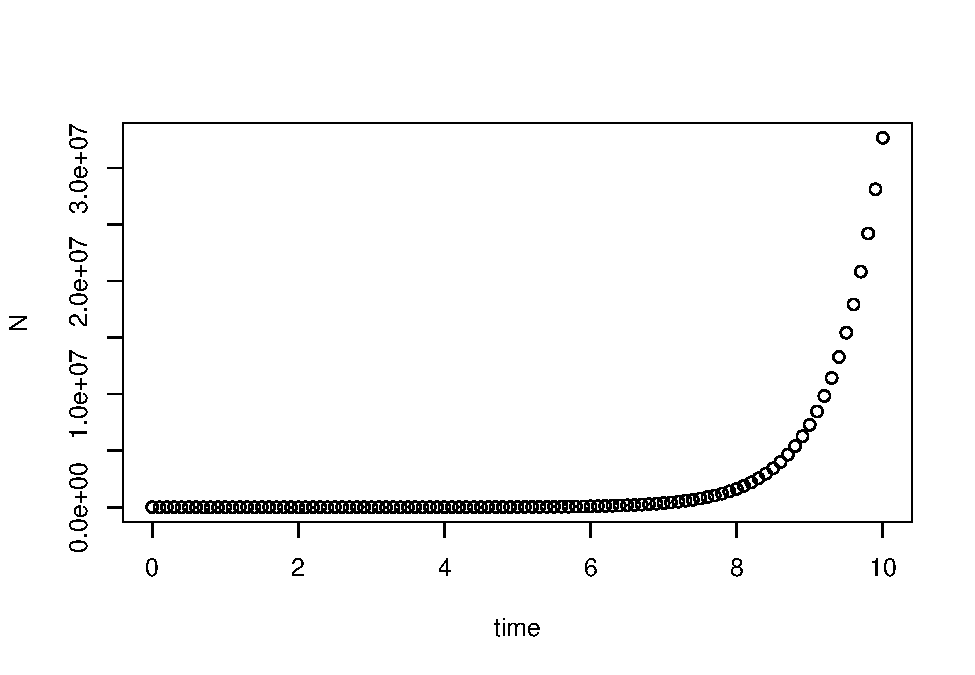
\includegraphics{bookdown-demo_files/figure-latex/unnamed-chunk-5-1.pdf}

Compare simulation result with analytic solution, which is
\[
N(t) = N_0\exp\{rt\}
\]

\begin{Shaded}
\begin{Highlighting}[]
\FunctionTok{par}\NormalTok{(}\AttributeTok{mfrow =} \FunctionTok{c}\NormalTok{(}\DecValTok{1}\NormalTok{,}\DecValTok{2}\NormalTok{))}
\FunctionTok{plot}\NormalTok{(N }\SpecialCharTok{\textasciitilde{}}\NormalTok{ time, }\AttributeTok{data =}\NormalTok{ pop\_size) }\CommentTok{\# Plot simulation data}
\FunctionTok{curve}\NormalTok{(state[}\DecValTok{1}\NormalTok{]}\SpecialCharTok{*}\FunctionTok{exp}\NormalTok{(parms[}\DecValTok{1}\NormalTok{]}\SpecialCharTok{*}\NormalTok{x), }\AttributeTok{col =} \StringTok{"red"}\NormalTok{, }\AttributeTok{add =}\NormalTok{ T) }\CommentTok{\# Adding analytic solution}
\FunctionTok{plot}\NormalTok{(N }\SpecialCharTok{\textasciitilde{}}\NormalTok{ time, }\AttributeTok{data =}\NormalTok{ pop\_size, }\AttributeTok{log =} \StringTok{"y"}\NormalTok{) }\CommentTok{\# Plot logged simulation data}
\FunctionTok{curve}\NormalTok{(state[}\DecValTok{1}\NormalTok{]}\SpecialCharTok{*}\FunctionTok{exp}\NormalTok{(parms[}\DecValTok{1}\NormalTok{]}\SpecialCharTok{*}\NormalTok{x), }\AttributeTok{col =} \StringTok{"red"}\NormalTok{, }\AttributeTok{add =}\NormalTok{ T) }\CommentTok{\# Adding analytic solution}
\end{Highlighting}
\end{Shaded}

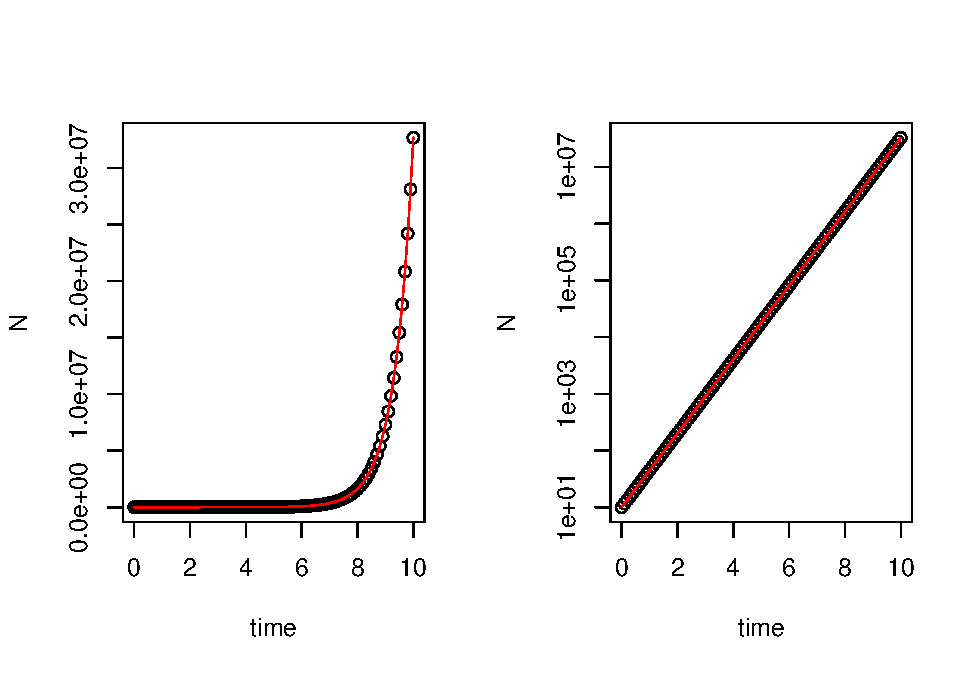
\includegraphics{bookdown-demo_files/figure-latex/unnamed-chunk-6-1.pdf}

\textbf{Part 2 - Comparing different ode solvers and different time intervals}
In default of \texttt{ode()}, the equations are solved by LSODA method. We can change the method by modifying the argument \texttt{method} in \texttt{ode()}.

\begin{Shaded}
\begin{Highlighting}[]
\DocumentationTok{\#\#\#\#\#\# part 2 \#\#\#\#\#\#}
\CommentTok{\# Original setting}
\NormalTok{times }\OtherTok{\textless{}{-}} \FunctionTok{seq}\NormalTok{(}\DecValTok{0}\NormalTok{, }\DecValTok{10}\NormalTok{, }\AttributeTok{by =} \FloatTok{0.1}\NormalTok{)  }\CommentTok{\# Time steps to integrate over}
\NormalTok{state }\OtherTok{\textless{}{-}} \FunctionTok{c}\NormalTok{(}\AttributeTok{N =} \DecValTok{10}\NormalTok{)  }\CommentTok{\# Initial population size}
\NormalTok{parms }\OtherTok{\textless{}{-}} \FunctionTok{c}\NormalTok{(}\AttributeTok{r =} \FloatTok{1.5}\NormalTok{)  }\CommentTok{\# Intrinsic growth rate}
\CommentTok{\# Default: LSODA}
\NormalTok{pop\_size }\OtherTok{\textless{}{-}} \FunctionTok{ode}\NormalTok{(}\AttributeTok{func =}\NormalTok{ exponential\_model, }\AttributeTok{times =}\NormalTok{ times, }\AttributeTok{y =}\NormalTok{ state, }\AttributeTok{parms =}\NormalTok{ parms)}

\CommentTok{\# Euler\textquotesingle{}s method}
\NormalTok{pop\_size\_1 }\OtherTok{\textless{}{-}} \FunctionTok{ode}\NormalTok{(}\AttributeTok{func =}\NormalTok{ exponential\_model, }\AttributeTok{times =}\NormalTok{ times, }\AttributeTok{y =}\NormalTok{ state, }\AttributeTok{parms =}\NormalTok{ parms, }\AttributeTok{method =} \StringTok{"euler"}\NormalTok{)}

\CommentTok{\# Compare different method}
\FunctionTok{par}\NormalTok{(}\AttributeTok{mfrow =} \FunctionTok{c}\NormalTok{(}\DecValTok{1}\NormalTok{,}\DecValTok{2}\NormalTok{))}
\FunctionTok{plot}\NormalTok{(N }\SpecialCharTok{\textasciitilde{}}\NormalTok{ time, }\AttributeTok{data =}\NormalTok{ pop\_size, }\AttributeTok{main =} \StringTok{"LSODA"}\NormalTok{)}
\FunctionTok{curve}\NormalTok{(state[}\DecValTok{1}\NormalTok{]}\SpecialCharTok{*}\FunctionTok{exp}\NormalTok{(parms[}\DecValTok{1}\NormalTok{]}\SpecialCharTok{*}\NormalTok{x), times[}\DecValTok{1}\NormalTok{], times[}\FunctionTok{length}\NormalTok{(times)], }\AttributeTok{col =} \StringTok{"red"}\NormalTok{, }\AttributeTok{add =}\NormalTok{ T) }\CommentTok{\# correct curve}
\FunctionTok{plot}\NormalTok{(N }\SpecialCharTok{\textasciitilde{}}\NormalTok{ time, }\AttributeTok{data =}\NormalTok{ pop\_size\_1, }\AttributeTok{main =} \StringTok{"Euler"}\NormalTok{)}
\FunctionTok{curve}\NormalTok{(state[}\DecValTok{1}\NormalTok{]}\SpecialCharTok{*}\FunctionTok{exp}\NormalTok{(parms[}\DecValTok{1}\NormalTok{]}\SpecialCharTok{*}\NormalTok{x), times[}\DecValTok{1}\NormalTok{], times[}\FunctionTok{length}\NormalTok{(times)], }\AttributeTok{col =} \StringTok{"red"}\NormalTok{, }\AttributeTok{add =}\NormalTok{ T) }\CommentTok{\# correct curve}
\end{Highlighting}
\end{Shaded}

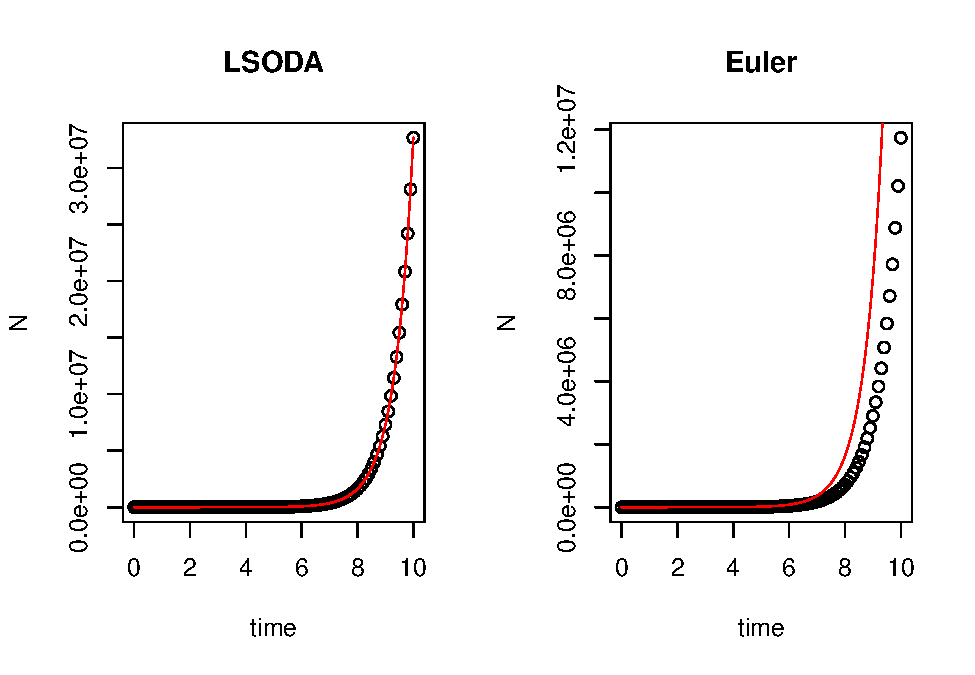
\includegraphics{bookdown-demo_files/figure-latex/unnamed-chunk-7-1.pdf}

\begin{Shaded}
\begin{Highlighting}[]
\CommentTok{\# Different time intervals}
\NormalTok{times\_1 }\OtherTok{\textless{}{-}} \FunctionTok{seq}\NormalTok{(}\DecValTok{0}\NormalTok{, }\DecValTok{10}\NormalTok{, }\AttributeTok{by =} \DecValTok{1}\NormalTok{)  }\CommentTok{\# time steps to integrate over}
\NormalTok{times\_2 }\OtherTok{\textless{}{-}} \FunctionTok{seq}\NormalTok{(}\DecValTok{0}\NormalTok{, }\DecValTok{10}\NormalTok{, }\AttributeTok{by =} \FloatTok{0.1}\NormalTok{)  }\CommentTok{\# time steps to integrate over}
\NormalTok{times\_3 }\OtherTok{\textless{}{-}} \FunctionTok{seq}\NormalTok{(}\DecValTok{0}\NormalTok{, }\DecValTok{10}\NormalTok{, }\AttributeTok{by =} \FloatTok{0.01}\NormalTok{)  }\CommentTok{\# time steps to integrate over}

\CommentTok{\# Euler\textquotesingle{}s method}
\NormalTok{pop\_size\_1 }\OtherTok{\textless{}{-}} \FunctionTok{ode}\NormalTok{(}\AttributeTok{func =}\NormalTok{ exponential\_model, }\AttributeTok{times =}\NormalTok{ times\_1, }\AttributeTok{y =}\NormalTok{ state, }\AttributeTok{parms =}\NormalTok{ parms, }\AttributeTok{method =} \StringTok{"euler"}\NormalTok{)}
\NormalTok{pop\_size\_2 }\OtherTok{\textless{}{-}} \FunctionTok{ode}\NormalTok{(}\AttributeTok{func =}\NormalTok{ exponential\_model, }\AttributeTok{times =}\NormalTok{ times\_2, }\AttributeTok{y =}\NormalTok{ state, }\AttributeTok{parms =}\NormalTok{ parms, }\AttributeTok{method =} \StringTok{"euler"}\NormalTok{)}
\NormalTok{pop\_size\_3 }\OtherTok{\textless{}{-}} \FunctionTok{ode}\NormalTok{(}\AttributeTok{func =}\NormalTok{ exponential\_model, }\AttributeTok{times =}\NormalTok{ times\_3, }\AttributeTok{y =}\NormalTok{ state, }\AttributeTok{parms =}\NormalTok{ parms, }\AttributeTok{method =} \StringTok{"euler"}\NormalTok{)}

\CommentTok{\# Compare different time intervals}
\FunctionTok{par}\NormalTok{(}\AttributeTok{mfrow =} \FunctionTok{c}\NormalTok{(}\DecValTok{1}\NormalTok{,}\DecValTok{3}\NormalTok{))}
\FunctionTok{plot}\NormalTok{(N }\SpecialCharTok{\textasciitilde{}}\NormalTok{ time, }\AttributeTok{data =}\NormalTok{ pop\_size\_1, }\AttributeTok{main =} \StringTok{"Time intervals = 1"}\NormalTok{)}
\FunctionTok{curve}\NormalTok{(state[}\DecValTok{1}\NormalTok{]}\SpecialCharTok{*}\FunctionTok{exp}\NormalTok{(parms[}\DecValTok{1}\NormalTok{]}\SpecialCharTok{*}\NormalTok{x), }\AttributeTok{col =} \StringTok{"red"}\NormalTok{, }\AttributeTok{add =}\NormalTok{ T) }\CommentTok{\# correct curve}
\FunctionTok{plot}\NormalTok{(N }\SpecialCharTok{\textasciitilde{}}\NormalTok{ time, }\AttributeTok{data =}\NormalTok{ pop\_size\_2, }\AttributeTok{main =} \StringTok{"Time intervals = 0.1"}\NormalTok{)}
\FunctionTok{curve}\NormalTok{(state[}\DecValTok{1}\NormalTok{]}\SpecialCharTok{*}\FunctionTok{exp}\NormalTok{(parms[}\DecValTok{1}\NormalTok{]}\SpecialCharTok{*}\NormalTok{x), }\AttributeTok{col =} \StringTok{"red"}\NormalTok{, }\AttributeTok{add =}\NormalTok{ T) }\CommentTok{\# correct curve}
\FunctionTok{plot}\NormalTok{(N }\SpecialCharTok{\textasciitilde{}}\NormalTok{ time, }\AttributeTok{data =}\NormalTok{ pop\_size\_3, }\AttributeTok{main =} \StringTok{"Time intervals = 0.01"}\NormalTok{)}
\FunctionTok{curve}\NormalTok{(state[}\DecValTok{1}\NormalTok{]}\SpecialCharTok{*}\FunctionTok{exp}\NormalTok{(parms[}\DecValTok{1}\NormalTok{]}\SpecialCharTok{*}\NormalTok{x), }\AttributeTok{col =} \StringTok{"red"}\NormalTok{, }\AttributeTok{add =}\NormalTok{ T) }\CommentTok{\# correct curve}
\end{Highlighting}
\end{Shaded}

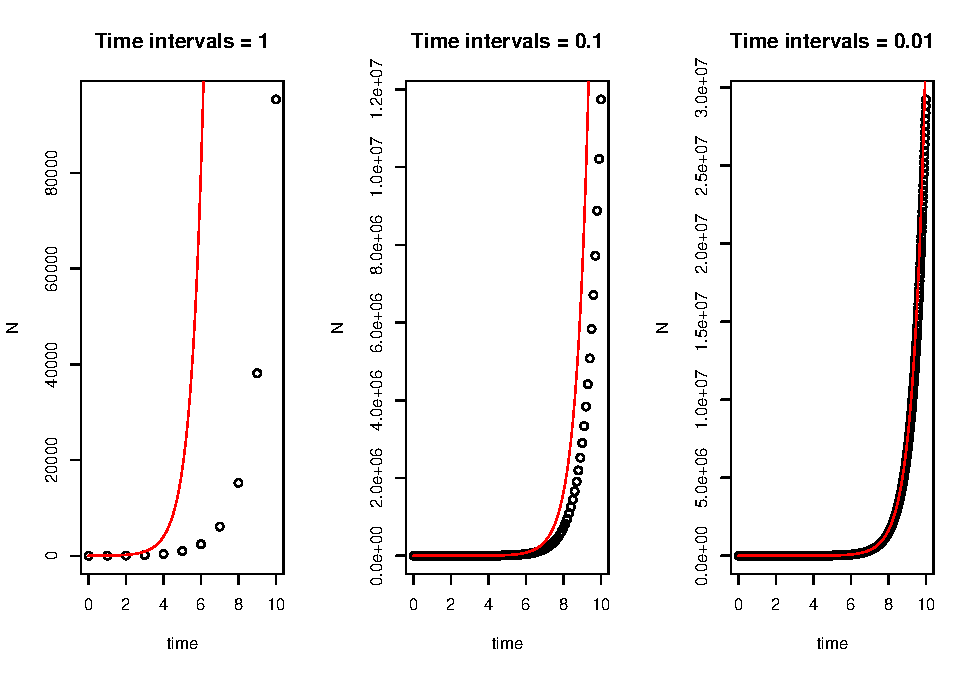
\includegraphics{bookdown-demo_files/figure-latex/unnamed-chunk-7-2.pdf}

\textbf{Part 3 - Solving exponential growth model with fluctuating growth rate}
Consider the model
\[
\frac{dN}{dt} = r(t)N \ \text{, } r(t) = \overline{r} + \sigma\sin(\omega t)
\]
where \(\overline{r}\) and \(\omega\) are constants.
The analytic solution of the ode model is
\[
N(t) = N_0\exp\{\overline{r}t - \frac{\sigma}{\omega}[\cos(\omega t) - 1]\}
\]

\begin{Shaded}
\begin{Highlighting}[]
\DocumentationTok{\#\#\#\#\#\# part 3 \#\#\#\#\#\#}
\DocumentationTok{\#\#\# Model specification}
\NormalTok{exponential\_model\_fluc }\OtherTok{\textless{}{-}} \ControlFlowTok{function}\NormalTok{(times, state, parms) \{}
  \FunctionTok{with}\NormalTok{(}\FunctionTok{as.list}\NormalTok{(}\FunctionTok{c}\NormalTok{(state, parms)), \{}
\NormalTok{    dN\_dt }\OtherTok{=}\NormalTok{ (r\_bar }\SpecialCharTok{+}\NormalTok{ sigma}\SpecialCharTok{*}\FunctionTok{sin}\NormalTok{(omega}\SpecialCharTok{*}\NormalTok{times))}\SpecialCharTok{*}\NormalTok{N  }\CommentTok{\# exponential growth equation}
    \FunctionTok{return}\NormalTok{(}\FunctionTok{list}\NormalTok{(}\FunctionTok{c}\NormalTok{(dN\_dt)))  }\CommentTok{\# return the results}
\NormalTok{  \})}
\NormalTok{\}}
\end{Highlighting}
\end{Shaded}

\begin{Shaded}
\begin{Highlighting}[]
\DocumentationTok{\#\#\# Parameters}
\NormalTok{times }\OtherTok{\textless{}{-}} \FunctionTok{seq}\NormalTok{(}\DecValTok{0}\NormalTok{, }\DecValTok{10}\NormalTok{, }\AttributeTok{by =} \FloatTok{0.1}\NormalTok{)  }\CommentTok{\# time steps to integrate over}
\NormalTok{state }\OtherTok{\textless{}{-}} \FunctionTok{c}\NormalTok{(}\AttributeTok{N =} \DecValTok{10}\NormalTok{)  }\CommentTok{\# initial population size}
\NormalTok{parms }\OtherTok{\textless{}{-}} \FunctionTok{c}\NormalTok{(}\AttributeTok{r\_bar =} \FloatTok{1.5}\NormalTok{, }\AttributeTok{sigma =} \DecValTok{5}\NormalTok{, }\AttributeTok{omega =} \DecValTok{2}\SpecialCharTok{*}\NormalTok{pi)  }\CommentTok{\# intrinsic growth rate}
\end{Highlighting}
\end{Shaded}

Plot \(r(t)\)

\begin{Shaded}
\begin{Highlighting}[]
\DocumentationTok{\#\#\# Fluctuating growth rate}
\NormalTok{r }\OtherTok{=}\NormalTok{ parms[}\DecValTok{1}\NormalTok{] }\SpecialCharTok{+}\NormalTok{ parms[}\DecValTok{2}\NormalTok{]}\SpecialCharTok{*}\FunctionTok{sin}\NormalTok{(parms[}\DecValTok{3}\NormalTok{]}\SpecialCharTok{*}\NormalTok{times)}
\FunctionTok{plot}\NormalTok{(r }\SpecialCharTok{\textasciitilde{}}\NormalTok{ times, }\AttributeTok{type =} \StringTok{"l"}\NormalTok{)}
\end{Highlighting}
\end{Shaded}

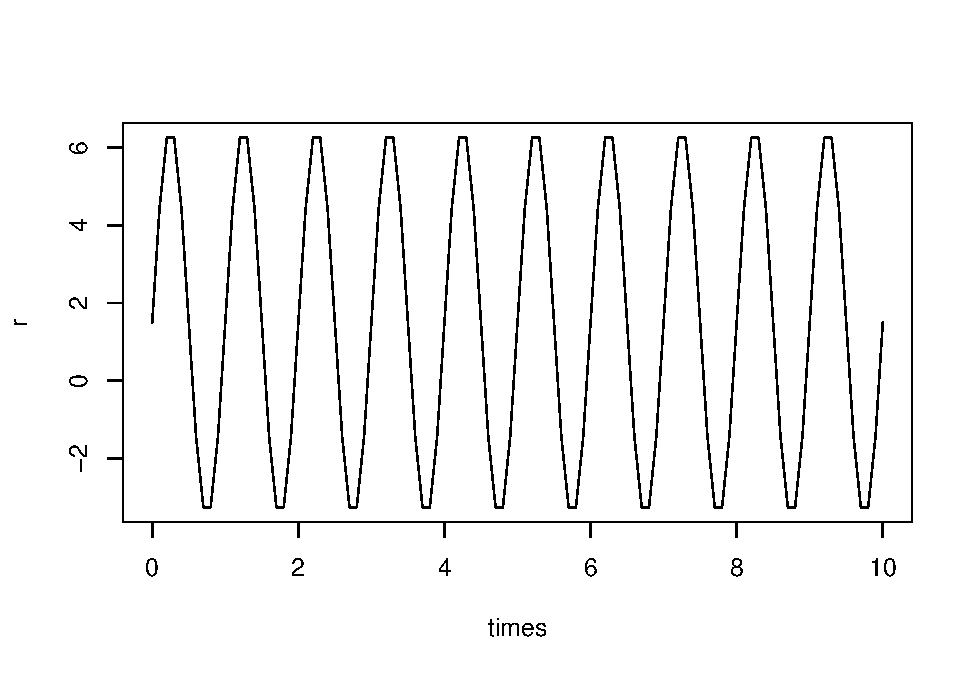
\includegraphics{bookdown-demo_files/figure-latex/unnamed-chunk-10-1.pdf}

\begin{Shaded}
\begin{Highlighting}[]
\DocumentationTok{\#\#\# Solving model}
\NormalTok{pop\_size }\OtherTok{\textless{}{-}} \FunctionTok{ode}\NormalTok{(}\AttributeTok{func =}\NormalTok{ exponential\_model\_fluc, }\AttributeTok{times =}\NormalTok{ times, }\AttributeTok{y =}\NormalTok{ state, }\AttributeTok{parms =}\NormalTok{ parms)}

\DocumentationTok{\#\#\# Plotting}
\FunctionTok{plot}\NormalTok{(N }\SpecialCharTok{\textasciitilde{}}\NormalTok{ times, }\AttributeTok{data =}\NormalTok{ pop\_size)}
\FunctionTok{curve}\NormalTok{(state[}\DecValTok{1}\NormalTok{]}\SpecialCharTok{*}\FunctionTok{exp}\NormalTok{(parms[}\DecValTok{1}\NormalTok{]}\SpecialCharTok{*}\NormalTok{x }\SpecialCharTok{{-}}\NormalTok{ parms[}\DecValTok{2}\NormalTok{]}\SpecialCharTok{/}\NormalTok{parms[}\DecValTok{3}\NormalTok{]}\SpecialCharTok{*}\NormalTok{(}\FunctionTok{cos}\NormalTok{(parms[}\DecValTok{3}\NormalTok{]}\SpecialCharTok{*}\NormalTok{x) }\SpecialCharTok{{-}} \DecValTok{1}\NormalTok{)), }\AttributeTok{add =}\NormalTok{ T, }\AttributeTok{col =} \StringTok{"red"}\NormalTok{) }\CommentTok{\# correct curve}
\end{Highlighting}
\end{Shaded}

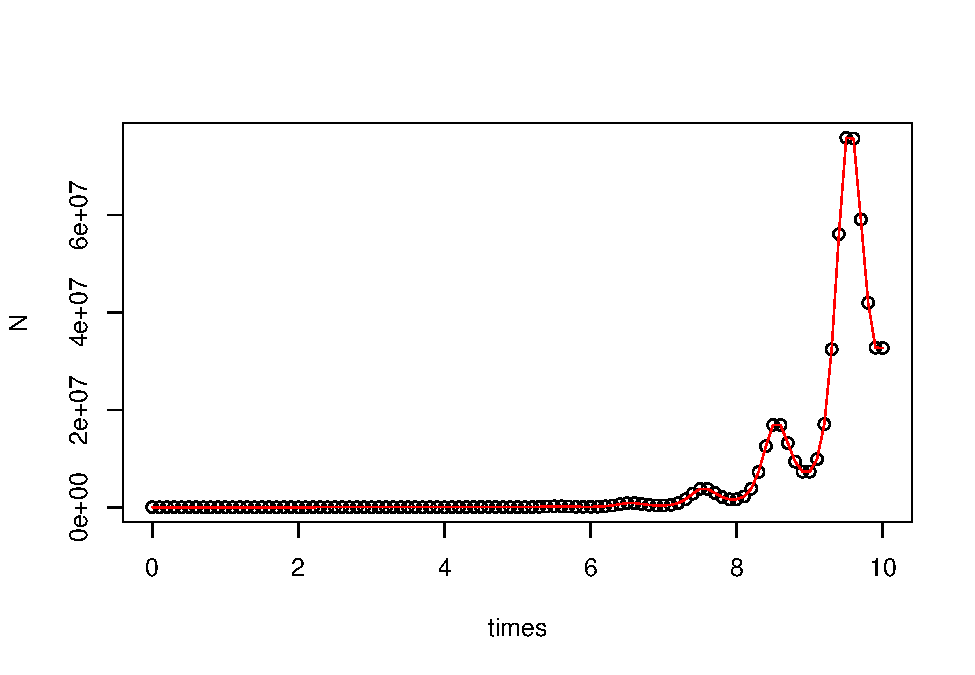
\includegraphics{bookdown-demo_files/figure-latex/unnamed-chunk-11-1.pdf}

\begin{Shaded}
\begin{Highlighting}[]
\FunctionTok{plot}\NormalTok{(N }\SpecialCharTok{\textasciitilde{}}\NormalTok{ times, }\AttributeTok{data =}\NormalTok{ pop\_size, }\AttributeTok{log =} \StringTok{"y"}\NormalTok{)}
\FunctionTok{curve}\NormalTok{(state[}\DecValTok{1}\NormalTok{]}\SpecialCharTok{*}\FunctionTok{exp}\NormalTok{(parms[}\DecValTok{1}\NormalTok{]}\SpecialCharTok{*}\NormalTok{x }\SpecialCharTok{{-}}\NormalTok{ parms[}\DecValTok{2}\NormalTok{]}\SpecialCharTok{/}\NormalTok{parms[}\DecValTok{3}\NormalTok{]}\SpecialCharTok{*}\NormalTok{(}\FunctionTok{cos}\NormalTok{(parms[}\DecValTok{3}\NormalTok{]}\SpecialCharTok{*}\NormalTok{x) }\SpecialCharTok{{-}} \DecValTok{1}\NormalTok{)), }\AttributeTok{add =}\NormalTok{ T, }\AttributeTok{col =} \StringTok{"red"}\NormalTok{) }\CommentTok{\# correct curve}
\end{Highlighting}
\end{Shaded}

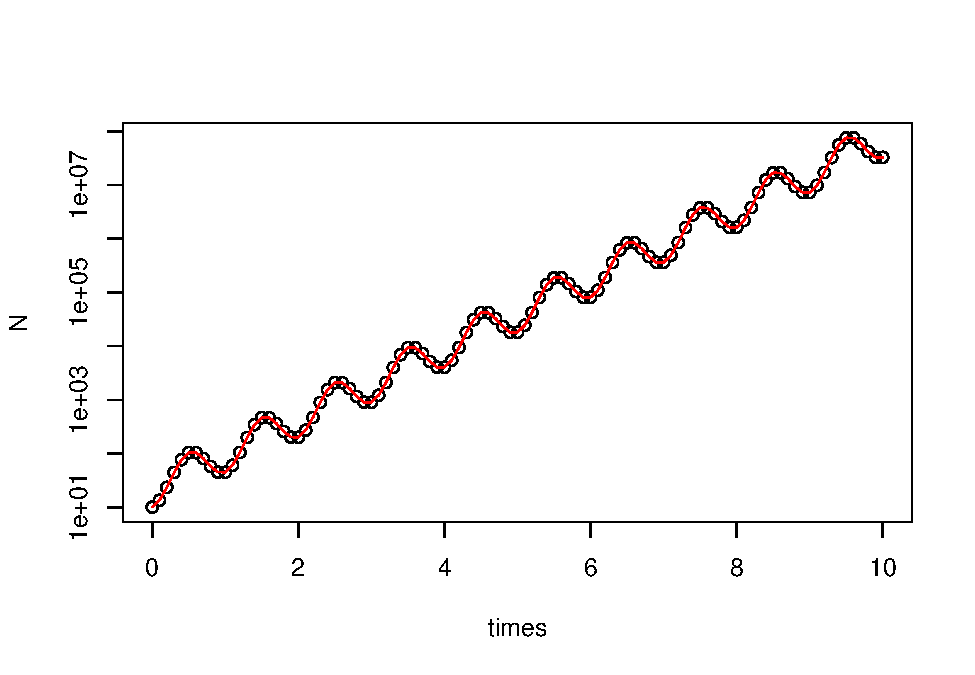
\includegraphics{bookdown-demo_files/figure-latex/unnamed-chunk-11-2.pdf}

Adjust \(\overline{r}\)

\begin{Shaded}
\begin{Highlighting}[]
\DocumentationTok{\#\#\# Parameters}
\NormalTok{times }\OtherTok{\textless{}{-}} \FunctionTok{seq}\NormalTok{(}\DecValTok{0}\NormalTok{, }\DecValTok{10}\NormalTok{, }\AttributeTok{by =} \FloatTok{0.1}\NormalTok{)  }\CommentTok{\# time steps to integrate over}
\NormalTok{state }\OtherTok{\textless{}{-}} \FunctionTok{c}\NormalTok{(}\AttributeTok{N =} \DecValTok{10}\NormalTok{)  }\CommentTok{\# initial population size}
\NormalTok{parms }\OtherTok{\textless{}{-}} \FunctionTok{c}\NormalTok{(}\AttributeTok{r\_bar =} \FloatTok{0.1}\NormalTok{, }\AttributeTok{sigma =} \DecValTok{5}\NormalTok{, }\AttributeTok{omega =} \DecValTok{2}\SpecialCharTok{*}\NormalTok{pi)  }\CommentTok{\# intrinsic growth rate}

\DocumentationTok{\#\#\# Fluctuating growth rate}
\NormalTok{r }\OtherTok{=}\NormalTok{ parms[}\DecValTok{1}\NormalTok{] }\SpecialCharTok{+}\NormalTok{ parms[}\DecValTok{2}\NormalTok{]}\SpecialCharTok{*}\FunctionTok{sin}\NormalTok{(parms[}\DecValTok{3}\NormalTok{]}\SpecialCharTok{*}\NormalTok{times)}
\FunctionTok{plot}\NormalTok{(r }\SpecialCharTok{\textasciitilde{}}\NormalTok{ times, }\AttributeTok{type =} \StringTok{"l"}\NormalTok{)}
\end{Highlighting}
\end{Shaded}

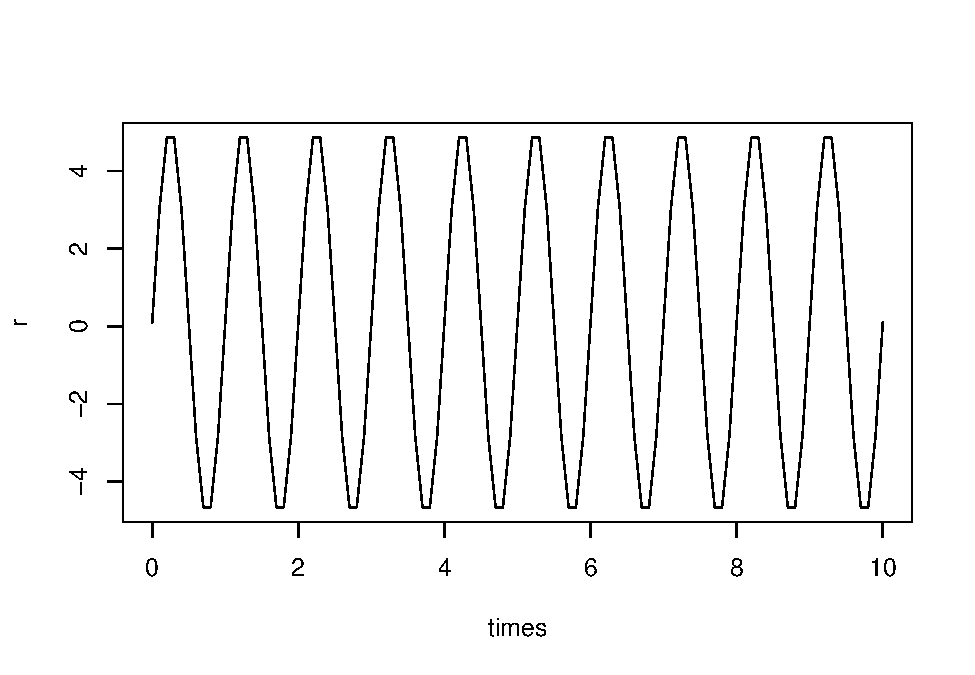
\includegraphics{bookdown-demo_files/figure-latex/unnamed-chunk-12-1.pdf}

\begin{Shaded}
\begin{Highlighting}[]
\DocumentationTok{\#\#\# Solving model}
\NormalTok{pop\_size }\OtherTok{\textless{}{-}} \FunctionTok{ode}\NormalTok{(}\AttributeTok{func =}\NormalTok{ exponential\_model\_fluc, }\AttributeTok{times =}\NormalTok{ times, }\AttributeTok{y =}\NormalTok{ state, }\AttributeTok{parms =}\NormalTok{ parms)}

\DocumentationTok{\#\#\# Plotting}
\FunctionTok{plot}\NormalTok{(N }\SpecialCharTok{\textasciitilde{}}\NormalTok{ times, }\AttributeTok{data =}\NormalTok{ pop\_size)}
\FunctionTok{curve}\NormalTok{(state[}\DecValTok{1}\NormalTok{]}\SpecialCharTok{*}\FunctionTok{exp}\NormalTok{(parms[}\DecValTok{1}\NormalTok{]}\SpecialCharTok{*}\NormalTok{x }\SpecialCharTok{{-}}\NormalTok{ parms[}\DecValTok{2}\NormalTok{]}\SpecialCharTok{/}\NormalTok{parms[}\DecValTok{3}\NormalTok{]}\SpecialCharTok{*}\NormalTok{(}\FunctionTok{cos}\NormalTok{(parms[}\DecValTok{3}\NormalTok{]}\SpecialCharTok{*}\NormalTok{x) }\SpecialCharTok{{-}} \DecValTok{1}\NormalTok{)), }\AttributeTok{add =}\NormalTok{ T, }\AttributeTok{col =} \StringTok{"red"}\NormalTok{) }\CommentTok{\# correct curve}
\end{Highlighting}
\end{Shaded}

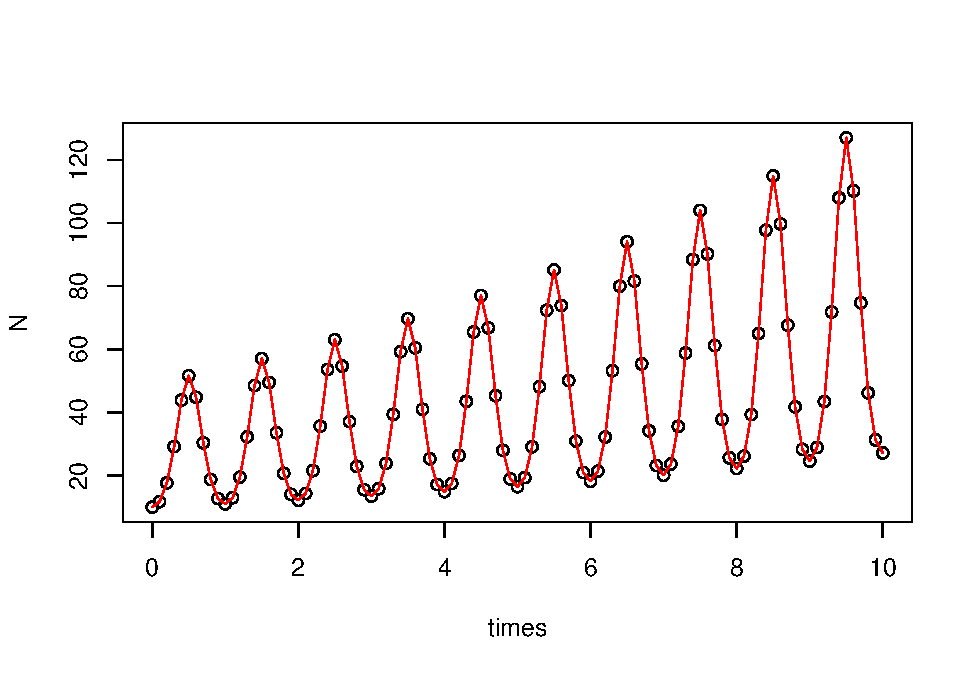
\includegraphics{bookdown-demo_files/figure-latex/unnamed-chunk-12-2.pdf}

\hypertarget{week-3---logistic-population-growth-and-stability-analysis}{%
\chapter*{Week 3 - Logistic population growth and stability analysis}\label{week-3---logistic-population-growth-and-stability-analysis}}
\addcontentsline{toc}{chapter}{Week 3 - Logistic population growth and stability analysis}

\textbf{Part 1 - Shining app for logistic growth}

Credit to \href{https://genchanghsu.github.io/index.html}{Gen-Chang Hsu}

\textbf{Part 2 - Population growth with Allee effects}

Some populations experience negative growth rates when the population size is too low, a phenomenon known as ``Allee effect''. For example, some flowering plants require a minimal local density to attract pollinators (clustering effects). Below this density, pollinators will not be able to detect the presence of flowers and therefore the plants cannot complete their life cycle. Some flower species, e.g., \emph{Itea}, requires a minimal population size of \(A\) to attract its specialized bee pollinator and its population growth is directly related to pollinator visitation, its population dynamics can be described using the below differential equation:

\[
\frac{dN}{dt} = rN(1-\frac{N}{K})(\frac{N}{A}-1)
\]

where \(0 < A < K\). The term \(A\) represents ``Allee threshold'', below which the population growth rate is negative (because of no visiting pollinators) and thus the population will decline; \(r\) is the intrinsic rate of increase and \(K\) is the carrying capacity.

\begin{enumerate}
\def\labelenumi{(\arabic{enumi})}
\tightlist
\item
  You can calculate the equilibrium population sizes and use the graphical method to determine their stability. The equilibrium population sizes are \(N^* = 0\) (stable), \(N^* = A\) (unstable), and \(N^* = K\) (stable).
\end{enumerate}

\begin{Shaded}
\begin{Highlighting}[]
\NormalTok{r }\OtherTok{=} \DecValTok{1}
\NormalTok{A }\OtherTok{=} \DecValTok{150}
\NormalTok{K }\OtherTok{=} \DecValTok{500}
\FunctionTok{curve}\NormalTok{(r}\SpecialCharTok{*}\NormalTok{x}\SpecialCharTok{*}\NormalTok{(}\DecValTok{1}\SpecialCharTok{{-}}\NormalTok{x}\SpecialCharTok{/}\NormalTok{K)}\SpecialCharTok{*}\NormalTok{(x}\SpecialCharTok{/}\NormalTok{A}\DecValTok{{-}1}\NormalTok{), }\AttributeTok{from =} \DecValTok{0}\NormalTok{, }\AttributeTok{to =} \DecValTok{550}\NormalTok{, }\AttributeTok{xlim =} \FunctionTok{c}\NormalTok{(}\DecValTok{0}\NormalTok{, }\DecValTok{550}\NormalTok{),}
      \AttributeTok{xlab =} \StringTok{"N"}\NormalTok{, }\AttributeTok{ylab =} \StringTok{"dN/dt"}\NormalTok{, }\AttributeTok{las =} \DecValTok{1}\NormalTok{)}
\FunctionTok{abline}\NormalTok{(}\AttributeTok{h =} \DecValTok{0}\NormalTok{, }\AttributeTok{lty =} \DecValTok{2}\NormalTok{)}
\FunctionTok{points}\NormalTok{(}\AttributeTok{y =} \FunctionTok{rep}\NormalTok{(}\DecValTok{0}\NormalTok{, }\DecValTok{3}\NormalTok{), }\AttributeTok{x =} \FunctionTok{c}\NormalTok{(}\DecValTok{0}\NormalTok{, A, K), }\AttributeTok{pch =} \FunctionTok{c}\NormalTok{(}\DecValTok{16}\NormalTok{, }\DecValTok{1}\NormalTok{, }\DecValTok{16}\NormalTok{))}
\FunctionTok{text}\NormalTok{(}\AttributeTok{x =} \FunctionTok{c}\NormalTok{(}\DecValTok{0}\NormalTok{, A, K), }\AttributeTok{y =} \FunctionTok{rep}\NormalTok{(}\DecValTok{20}\NormalTok{, }\DecValTok{3}\NormalTok{), }\AttributeTok{labels =} \FunctionTok{c}\NormalTok{(}\StringTok{"0"}\NormalTok{, }\StringTok{"A"}\NormalTok{, }\StringTok{"K"}\NormalTok{), }\AttributeTok{font =} \DecValTok{3}\NormalTok{, }\AttributeTok{col =} \StringTok{"blue"}\NormalTok{)}
\FunctionTok{arrows}\NormalTok{(}\AttributeTok{x0 =} \FunctionTok{c}\NormalTok{(}\DecValTok{100}\NormalTok{, }\DecValTok{200}\NormalTok{, }\DecValTok{550}\NormalTok{), }\AttributeTok{y0 =} \SpecialCharTok{{-}}\DecValTok{10}\NormalTok{, }\AttributeTok{x1 =} \FunctionTok{c}\NormalTok{(}\DecValTok{10}\NormalTok{, }\DecValTok{450}\NormalTok{, }\DecValTok{510}\NormalTok{), }\AttributeTok{y1 =} \SpecialCharTok{{-}}\DecValTok{10}\NormalTok{, }\AttributeTok{length =} \FloatTok{0.08}\NormalTok{, }\AttributeTok{lwd =} \DecValTok{2}\NormalTok{)}
\end{Highlighting}
\end{Shaded}

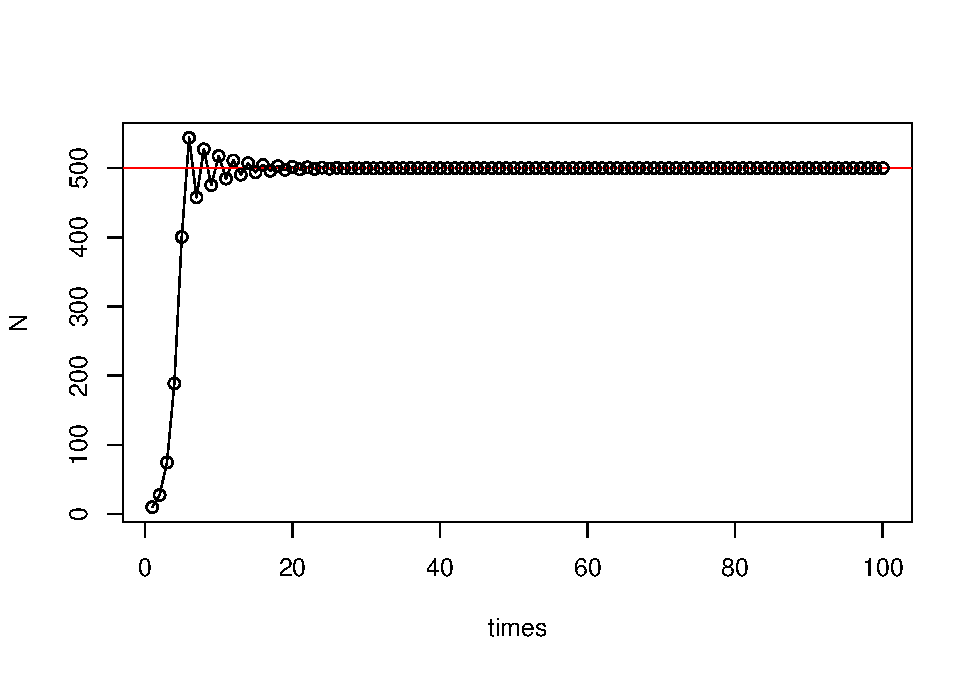
\includegraphics{bookdown-demo_files/figure-latex/unnamed-chunk-14-1.pdf}

\begin{enumerate}
\def\labelenumi{(\arabic{enumi})}
\setcounter{enumi}{1}
\tightlist
\item
  Simulate the dynamics with an intrinsic rate of increase of \(r\) = 1.2, the carrying capacity of \(K\) = 1000, and the minimal threshold density of \(A\) = 150. Observe the population trajectories to see how different initial population sizes can lead to different equilibrium population sizes (a phenomenon known as ``alternative stable states'').
\end{enumerate}

\begin{Shaded}
\begin{Highlighting}[]
\FunctionTok{library}\NormalTok{(deSolve)}
\NormalTok{Allee }\OtherTok{\textless{}{-}} \ControlFlowTok{function}\NormalTok{(t, state, pars) \{}
  \FunctionTok{with}\NormalTok{(}\FunctionTok{as.list}\NormalTok{(}\FunctionTok{c}\NormalTok{(state, pars)), \{}
\NormalTok{    dN\_dt }\OtherTok{=}\NormalTok{ r}\SpecialCharTok{*}\NormalTok{N}\SpecialCharTok{*}\NormalTok{(}\DecValTok{1}\SpecialCharTok{{-}}\NormalTok{N}\SpecialCharTok{/}\NormalTok{K)}\SpecialCharTok{*}\NormalTok{(N}\SpecialCharTok{/}\NormalTok{A}\DecValTok{{-}1}\NormalTok{)}
    \FunctionTok{return}\NormalTok{(}\FunctionTok{list}\NormalTok{(}\FunctionTok{c}\NormalTok{(dN\_dt)))}
\NormalTok{    \})}
\NormalTok{\}}
\NormalTok{t }\OtherTok{\textless{}{-}} \FunctionTok{seq}\NormalTok{(}\DecValTok{0}\NormalTok{, }\DecValTok{7}\NormalTok{, }\AttributeTok{by =} \FloatTok{0.01}\NormalTok{)}

\NormalTok{state }\OtherTok{\textless{}{-}} \FunctionTok{c}\NormalTok{(}\DecValTok{120}\NormalTok{,}\DecValTok{180}\NormalTok{, }\DecValTok{300}\NormalTok{, }\DecValTok{600}\NormalTok{, }\DecValTok{900}\NormalTok{, }\DecValTok{1200}\NormalTok{)}
\FunctionTok{names}\NormalTok{(state) }\OtherTok{\textless{}{-}} \FunctionTok{rep}\NormalTok{(}\StringTok{"N"}\NormalTok{, }\AttributeTok{time =} \FunctionTok{length}\NormalTok{(state))}
\NormalTok{pars }\OtherTok{\textless{}{-}} \FunctionTok{c}\NormalTok{(}\AttributeTok{r =} \FloatTok{1.2}\NormalTok{, }\AttributeTok{A =} \DecValTok{150}\NormalTok{, }\AttributeTok{K =} \DecValTok{1000}\NormalTok{)}
\FunctionTok{par}\NormalTok{(}\AttributeTok{mar =} \FunctionTok{c}\NormalTok{(}\DecValTok{5}\NormalTok{, }\DecValTok{4}\SpecialCharTok{+}\DecValTok{2}\NormalTok{, }\DecValTok{4}\NormalTok{,}\DecValTok{2}\NormalTok{) }\SpecialCharTok{+} \FloatTok{0.1}\NormalTok{)}

\ControlFlowTok{for}\NormalTok{(i }\ControlFlowTok{in} \DecValTok{1}\SpecialCharTok{:}\FunctionTok{length}\NormalTok{(state))\{}
  \CommentTok{\#runthe ode solver}
\NormalTok{  pop\_size }\OtherTok{\textless{}{-}} \FunctionTok{ode}\NormalTok{(}\AttributeTok{func =}\NormalTok{ Allee, }\AttributeTok{t =}\NormalTok{ t, }\AttributeTok{y =}\NormalTok{ state[i], }\AttributeTok{par =}\NormalTok{ pars)}
  \FunctionTok{plot}\NormalTok{(pop\_size,}\AttributeTok{ann =}\NormalTok{ F, }\AttributeTok{las =}\NormalTok{T, }\AttributeTok{ylim =} \FunctionTok{c}\NormalTok{(}\DecValTok{0}\NormalTok{, }\DecValTok{1500}\NormalTok{), }\AttributeTok{xlim =} \FunctionTok{c}\NormalTok{(}\FloatTok{0.2}\NormalTok{,}\DecValTok{7}\NormalTok{))}
  \FunctionTok{par}\NormalTok{(}\AttributeTok{new =} \ConstantTok{TRUE}\NormalTok{)}
\NormalTok{\}}
\FunctionTok{abline}\NormalTok{(}\AttributeTok{h =} \DecValTok{1000}\NormalTok{, }\AttributeTok{col =} \StringTok{"red"}\NormalTok{, }\AttributeTok{lty =} \DecValTok{2}\NormalTok{)}
\FunctionTok{abline}\NormalTok{(}\AttributeTok{h =} \DecValTok{150}\NormalTok{, }\AttributeTok{col =} \StringTok{"red"}\NormalTok{, }\AttributeTok{lty =} \DecValTok{2}\NormalTok{)}
\FunctionTok{axis}\NormalTok{(}\AttributeTok{side =} \DecValTok{2}\NormalTok{, }\AttributeTok{at =} \DecValTok{150}\NormalTok{, }\AttributeTok{las =}\NormalTok{ T)}
\FunctionTok{title}\NormalTok{(}\AttributeTok{main =} \FunctionTok{paste0}\NormalTok{(}\StringTok{"Allee effect}\SpecialCharTok{\textbackslash{}n}\StringTok{(r = "}\NormalTok{,pars[}\StringTok{"r"}\NormalTok{],}
                  \StringTok{", A = "}\NormalTok{,pars[}\StringTok{"A"}\NormalTok{],}
                  \StringTok{", K = "}\NormalTok{,pars[}\StringTok{"K"}\NormalTok{], }\StringTok{")"}\NormalTok{),}
      \AttributeTok{xlab =} \StringTok{"Time"}\NormalTok{)}
\FunctionTok{title}\NormalTok{(}\AttributeTok{ylab =} \StringTok{"Numberof individuals"}\NormalTok{, }\AttributeTok{line =} \DecValTok{4}\NormalTok{)}
\end{Highlighting}
\end{Shaded}

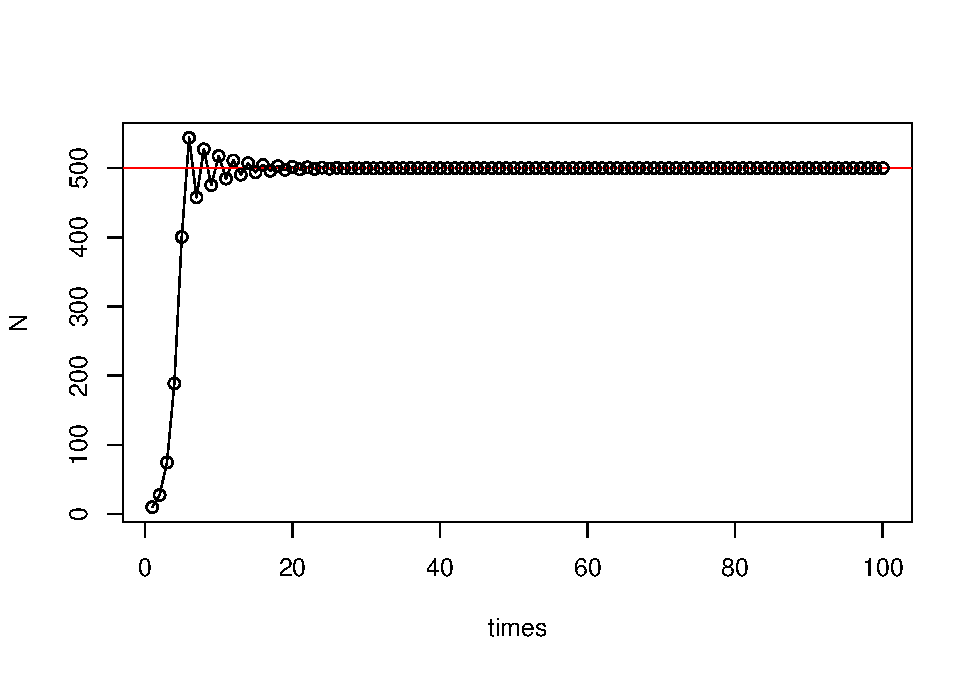
\includegraphics{bookdown-demo_files/figure-latex/unnamed-chunk-15-1.pdf}

\hypertarget{week-4---discrete-exponential-and-logistic-models}{%
\chapter*{Week 4 - Discrete exponential and logistic models}\label{week-4---discrete-exponential-and-logistic-models}}
\addcontentsline{toc}{chapter}{Week 4 - Discrete exponential and logistic models}

\textbf{Part 1 - Model the discrete logistic population growth using for loops}
Model:
\[
N_{t+1} = N_t(1+r(1-\frac{N_t}{K}))
\]

\begin{Shaded}
\begin{Highlighting}[]
\DocumentationTok{\#\#\# (1) Define the discrete logistic growth equation}
\NormalTok{log\_fun }\OtherTok{\textless{}{-}} \ControlFlowTok{function}\NormalTok{(r, N, K)\{N }\SpecialCharTok{+}\NormalTok{ r}\SpecialCharTok{*}\NormalTok{N}\SpecialCharTok{*}\NormalTok{(}\DecValTok{1}\SpecialCharTok{{-}}\NormalTok{N}\SpecialCharTok{/}\NormalTok{K)\}}
\end{Highlighting}
\end{Shaded}

You may modify \(r\) to see the change in stability of equilibrium \(K\).

\begin{Shaded}
\begin{Highlighting}[]
\DocumentationTok{\#\#\# (2) Set the parameters}
\NormalTok{r }\OtherTok{\textless{}{-}} \FloatTok{1.8}
\NormalTok{K }\OtherTok{\textless{}{-}} \DecValTok{200}
\NormalTok{N0 }\OtherTok{\textless{}{-}} \DecValTok{10}
\NormalTok{time }\OtherTok{\textless{}{-}} \DecValTok{100}
\NormalTok{Parms }\OtherTok{\textless{}{-}} \FunctionTok{c}\NormalTok{(}\AttributeTok{r =}\NormalTok{ r, }\AttributeTok{K =}\NormalTok{ K)}

\DocumentationTok{\#\#\# (3) Use for loop to iterate over the time sequence}
\NormalTok{pop\_size }\OtherTok{\textless{}{-}} \FunctionTok{data.frame}\NormalTok{(}\AttributeTok{times =} \DecValTok{1}\SpecialCharTok{:}\NormalTok{time)}
\NormalTok{pop\_size}\SpecialCharTok{$}\NormalTok{N[}\DecValTok{1}\NormalTok{] }\OtherTok{\textless{}{-}}\NormalTok{ N0}
\ControlFlowTok{for}\NormalTok{(i }\ControlFlowTok{in} \DecValTok{2}\SpecialCharTok{:}\NormalTok{time)\{}
\NormalTok{  pop\_size}\SpecialCharTok{$}\NormalTok{N[i] }\OtherTok{\textless{}{-}} \FunctionTok{log\_fun}\NormalTok{(}\AttributeTok{r =}\NormalTok{ r, }\AttributeTok{N =}\NormalTok{ pop\_size}\SpecialCharTok{$}\NormalTok{N[i }\SpecialCharTok{{-}} \DecValTok{1}\NormalTok{], }\AttributeTok{K =}\NormalTok{ K)}
\NormalTok{\}}

\DocumentationTok{\#\#\# (4) Population trajectory}
\FunctionTok{plot}\NormalTok{(N }\SpecialCharTok{\textasciitilde{}}\NormalTok{ times, }\AttributeTok{data =}\NormalTok{ pop\_size, }\AttributeTok{type =} \StringTok{"l"}\NormalTok{)}
\FunctionTok{abline}\NormalTok{(}\AttributeTok{h =}\NormalTok{ K, }\AttributeTok{col =} \StringTok{"red"}\NormalTok{)}
\FunctionTok{points}\NormalTok{(N }\SpecialCharTok{\textasciitilde{}}\NormalTok{ times, }\AttributeTok{data =}\NormalTok{ pop\_size)}
\end{Highlighting}
\end{Shaded}

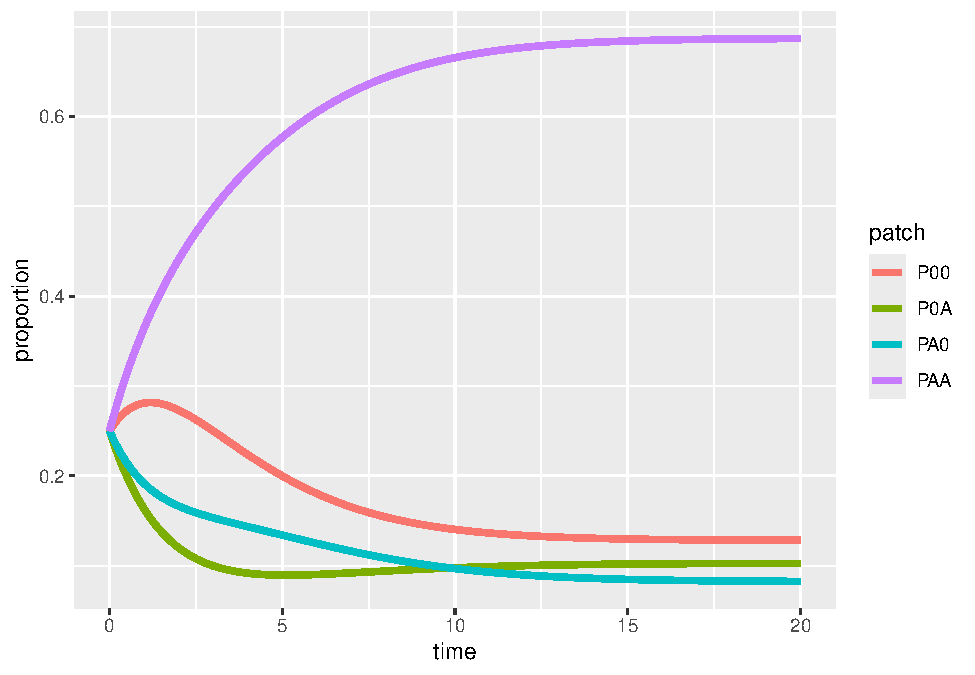
\includegraphics{bookdown-demo_files/figure-latex/unnamed-chunk-17-1.pdf}

\textbf{Part 2 - Generic cobweb}

\begin{Shaded}
\begin{Highlighting}[]
\DocumentationTok{\#\#\#\#\#\# Part 2: Generic cobweb}
\DocumentationTok{\#\#\# (1) define function}
\NormalTok{ReturnMap }\OtherTok{\textless{}{-}} \ControlFlowTok{function}\NormalTok{(Func, x0, times, xmax, }\AttributeTok{curve\_n =} \DecValTok{1000}\NormalTok{, parms)\{}
  
  \CommentTok{\# get time series iteration}
\NormalTok{  x }\OtherTok{\textless{}{-}} \FunctionTok{rep}\NormalTok{(x0, times)}
  \ControlFlowTok{for}\NormalTok{(i }\ControlFlowTok{in} \DecValTok{2}\SpecialCharTok{:}\NormalTok{times)\{}
\NormalTok{    x[i] }\OtherTok{\textless{}{-}} \FunctionTok{Func}\NormalTok{(x[i}\DecValTok{{-}1}\NormalTok{], parms)}
\NormalTok{  \}}
  
  \CommentTok{\# get fine grid for function curve}
\NormalTok{  x.grid }\OtherTok{\textless{}{-}} \FunctionTok{seq}\NormalTok{(}\DecValTok{0}\NormalTok{, xmax, }\AttributeTok{length.out =}\NormalTok{ curve\_n)}
\NormalTok{  y.grid }\OtherTok{\textless{}{-}} \FunctionTok{Func}\NormalTok{(x.grid, parms)}
\NormalTok{  ymax }\OtherTok{\textless{}{-}} \FunctionTok{max}\NormalTok{(y.grid, xmax)}
  
  \CommentTok{\# create canvas}
  \FunctionTok{plot}\NormalTok{(}\ConstantTok{NA}\NormalTok{, }\AttributeTok{xlim =} \FunctionTok{c}\NormalTok{(}\DecValTok{0}\NormalTok{, xmax), }\AttributeTok{ylim =} \FunctionTok{c}\NormalTok{(}\DecValTok{0}\NormalTok{, ymax), }\AttributeTok{xaxs =} \StringTok{"i"}\NormalTok{, }\AttributeTok{yaxs =} \StringTok{"i"}\NormalTok{, }\AttributeTok{bty =} \StringTok{"l"}\NormalTok{, }
       \AttributeTok{xlab =} \FunctionTok{expression}\NormalTok{(N[t]), }\AttributeTok{ylab =} \FunctionTok{expression}\NormalTok{(N[t}\SpecialCharTok{+}\DecValTok{1}\NormalTok{]))}
  \FunctionTok{abline}\NormalTok{(}\AttributeTok{a =} \DecValTok{0}\NormalTok{, }\AttributeTok{b =} \DecValTok{1}\NormalTok{, }\AttributeTok{lty =} \DecValTok{2}\NormalTok{, }\AttributeTok{col =} \StringTok{"grey50"}\NormalTok{)          }
  \FunctionTok{lines}\NormalTok{(x.grid, y.grid, }\AttributeTok{col =} \StringTok{"steelblue"}\NormalTok{, }\AttributeTok{lwd =} \DecValTok{2}\NormalTok{)      }
  
  \CommentTok{\# cobweb (horizontal to diagonal, vertical up to function)}
  \FunctionTok{segments}\NormalTok{(}\AttributeTok{x0 =}\NormalTok{ x[}\DecValTok{1}\NormalTok{], }\AttributeTok{y0 =} \DecValTok{0}\NormalTok{,   }\AttributeTok{x1 =}\NormalTok{ x[}\DecValTok{1}\NormalTok{],   }\AttributeTok{y1 =}\NormalTok{ x[}\DecValTok{2}\NormalTok{], }\AttributeTok{col =} \StringTok{"firebrick"}\NormalTok{)}
  \ControlFlowTok{for}\NormalTok{(i }\ControlFlowTok{in} \DecValTok{2}\SpecialCharTok{:}\NormalTok{(times}\DecValTok{{-}1}\NormalTok{))\{}
    \FunctionTok{segments}\NormalTok{(}\AttributeTok{x0 =}\NormalTok{ x[i}\DecValTok{{-}1}\NormalTok{], }\AttributeTok{y0 =}\NormalTok{ x[i],   }
             \AttributeTok{x1 =}\NormalTok{ x[i],   }\AttributeTok{y1 =}\NormalTok{ x[i], }\AttributeTok{col =} \StringTok{"firebrick"}\NormalTok{)}
    \FunctionTok{segments}\NormalTok{(}\AttributeTok{x0 =}\NormalTok{ x[i],   }\AttributeTok{y0 =}\NormalTok{ x[i], }
             \AttributeTok{x1 =}\NormalTok{ x[i],   }\AttributeTok{y1 =}\NormalTok{ x[i}\SpecialCharTok{+}\DecValTok{1}\NormalTok{], }\AttributeTok{col =} \StringTok{"firebrick"}\NormalTok{)}
\NormalTok{  \}}
  
\NormalTok{\}}

\DocumentationTok{\#\#\# (2) Set up discrete logistic function with outside parameters}
\NormalTok{Logistic }\OtherTok{\textless{}{-}} \ControlFlowTok{function}\NormalTok{(N, parms)\{}
  \FunctionTok{with}\NormalTok{(}\FunctionTok{as.list}\NormalTok{(parms), \{}
    \FunctionTok{return}\NormalTok{(N }\SpecialCharTok{+}\NormalTok{ r}\SpecialCharTok{*}\NormalTok{N}\SpecialCharTok{*}\NormalTok{(}\DecValTok{1}\SpecialCharTok{{-}}\NormalTok{N}\SpecialCharTok{/}\NormalTok{K))}
\NormalTok{  \})}
\NormalTok{\}}
\NormalTok{Parms }\OtherTok{\textless{}{-}} \FunctionTok{c}\NormalTok{(}\AttributeTok{r =}\NormalTok{ r, }\AttributeTok{K =}\NormalTok{ K)}

\DocumentationTok{\#\#\# (3) Use the ReturnMap function}
\FunctionTok{ReturnMap}\NormalTok{(}\AttributeTok{Func =}\NormalTok{ Logistic,}
          \AttributeTok{x0 =} \DecValTok{10}\NormalTok{, }
          \AttributeTok{times =} \DecValTok{150}\NormalTok{,}
          \AttributeTok{xmax =} \DecValTok{310}\NormalTok{,}
          \AttributeTok{curve\_n =} \DecValTok{1000}\NormalTok{, }
          \AttributeTok{parms =}\NormalTok{ Parms)}
\end{Highlighting}
\end{Shaded}

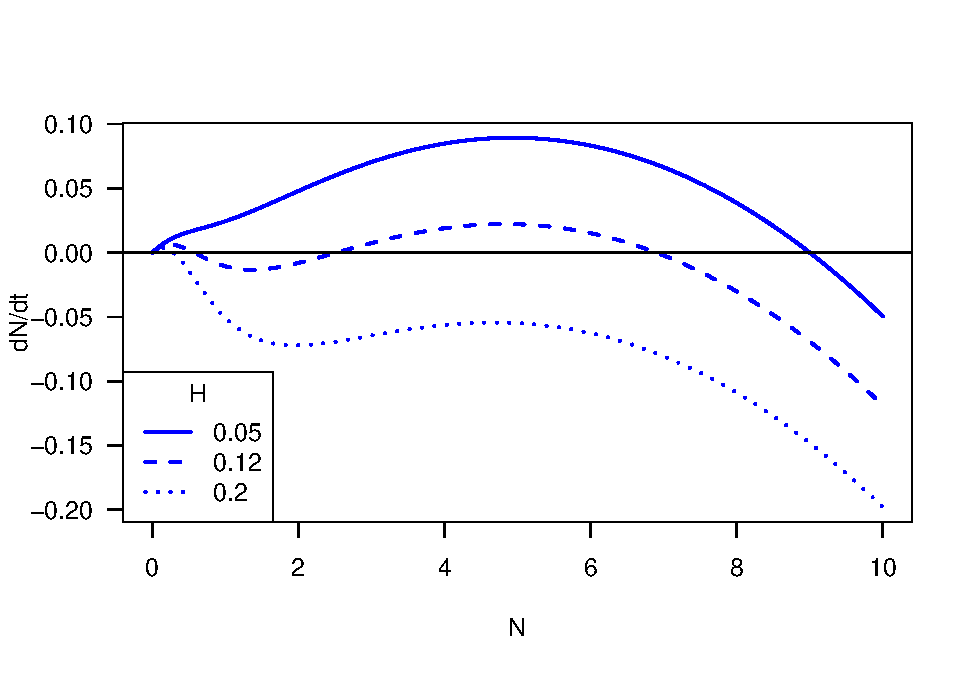
\includegraphics{bookdown-demo_files/figure-latex/unnamed-chunk-18-1.pdf}

Here is a shiny app for the discrete logistic growth model.

Credit to \href{https://genchanghsu.github.io/index.html}{Gen-Chang Hsu}

\textbf{Part 3 - Bifurcation}

\begin{Shaded}
\begin{Highlighting}[]
\DocumentationTok{\#\#\#\#\# Part 3: Logistic map and bifurcation}
\DocumentationTok{\#\#\# (1) Define the function}
\NormalTok{RickerPlot }\OtherTok{\textless{}{-}} \ControlFlowTok{function}\NormalTok{(Func, variable, var\_vec, x0, times, }\AttributeTok{x\_print =} \DecValTok{200}\NormalTok{, parms)\{}
  
  \CommentTok{\# prepare saving space }
\NormalTok{  data\_plot }\OtherTok{\textless{}{-}} \FunctionTok{data.frame}\NormalTok{(}\AttributeTok{var =} \FunctionTok{rep}\NormalTok{(var\_vec, }\AttributeTok{each =}\NormalTok{ x\_print), }\AttributeTok{x =} \DecValTok{0}\NormalTok{)}
  
  \CommentTok{\# change bifurcation parameter}
  \ControlFlowTok{for}\NormalTok{ (k }\ControlFlowTok{in} \DecValTok{1}\SpecialCharTok{:}\FunctionTok{length}\NormalTok{(var\_vec))\{}
\NormalTok{    parms[variable] }\OtherTok{\textless{}{-}}\NormalTok{ var\_vec[k]}
\NormalTok{    x }\OtherTok{\textless{}{-}} \FunctionTok{rep}\NormalTok{(x0, times)}
    
    \CommentTok{\# get time series with new bifurcation parameter}
    \ControlFlowTok{for}\NormalTok{(i }\ControlFlowTok{in} \DecValTok{2}\SpecialCharTok{:}\NormalTok{times)\{}
\NormalTok{      x[i] }\OtherTok{\textless{}{-}} \FunctionTok{Func}\NormalTok{(x[i}\DecValTok{{-}1}\NormalTok{], parms)}
\NormalTok{    \}}
    
    \CommentTok{\# save the data}
\NormalTok{    data\_plot}\SpecialCharTok{$}\NormalTok{x[(}\DecValTok{1} \SpecialCharTok{+}\NormalTok{ (k }\SpecialCharTok{{-}} \DecValTok{1}\NormalTok{)}\SpecialCharTok{*}\NormalTok{x\_print)}\SpecialCharTok{:}\NormalTok{(k}\SpecialCharTok{*}\NormalTok{x\_print)] }\OtherTok{\textless{}{-}}\NormalTok{ x[(times }\SpecialCharTok{{-}}\NormalTok{ x\_print }\SpecialCharTok{+} \DecValTok{1}\NormalTok{)}\SpecialCharTok{:}\NormalTok{times]}
\NormalTok{  \}}
  
  \CommentTok{\# plot }
  \FunctionTok{plot}\NormalTok{(x }\SpecialCharTok{\textasciitilde{}}\NormalTok{ var, }\AttributeTok{data =}\NormalTok{ data\_plot, }\AttributeTok{cex =} \FloatTok{0.05}\NormalTok{, }\AttributeTok{pch =} \DecValTok{20}\NormalTok{, }
       \AttributeTok{xlab =}\NormalTok{ variable, }\AttributeTok{ylab =} \StringTok{"Population size"}\NormalTok{)}
  
\NormalTok{\}}

\DocumentationTok{\#\#\#\# Discrete logistic function with outside parameters}
\NormalTok{Logistic }\OtherTok{\textless{}{-}} \ControlFlowTok{function}\NormalTok{(N, parms)\{}
  \FunctionTok{with}\NormalTok{(}\FunctionTok{as.list}\NormalTok{(parms), \{}
    \FunctionTok{return}\NormalTok{(N }\SpecialCharTok{+}\NormalTok{ r}\SpecialCharTok{*}\NormalTok{N}\SpecialCharTok{*}\NormalTok{(}\DecValTok{1}\SpecialCharTok{{-}}\NormalTok{N}\SpecialCharTok{/}\NormalTok{K))}
\NormalTok{  \})}
\NormalTok{\}}

\DocumentationTok{\#\#\# (2) Parameter setting}
\NormalTok{Parms }\OtherTok{\textless{}{-}} \FunctionTok{c}\NormalTok{(}\AttributeTok{r =}\NormalTok{ r, }\AttributeTok{K =}\NormalTok{ K)}
\NormalTok{r\_seq }\OtherTok{\textless{}{-}} \FunctionTok{seq}\NormalTok{(}\AttributeTok{from =} \FloatTok{1.8}\NormalTok{, }\AttributeTok{to =} \DecValTok{3}\NormalTok{, }\AttributeTok{by =} \FloatTok{0.001}\NormalTok{)}

\DocumentationTok{\#\#\# (3) Use generic ricker plot function}
\FunctionTok{RickerPlot}\NormalTok{(}\AttributeTok{Func =}\NormalTok{ Logistic, }
           \AttributeTok{variable =} \StringTok{"r"}\NormalTok{, }
           \AttributeTok{var\_vec =}\NormalTok{ r\_seq, }
           \AttributeTok{x0 =} \DecValTok{10}\NormalTok{, }
           \AttributeTok{times =} \DecValTok{500}\NormalTok{, }
           \AttributeTok{x\_print =} \DecValTok{100}\NormalTok{, }
           \AttributeTok{parms =}\NormalTok{ Parms)}
\end{Highlighting}
\end{Shaded}

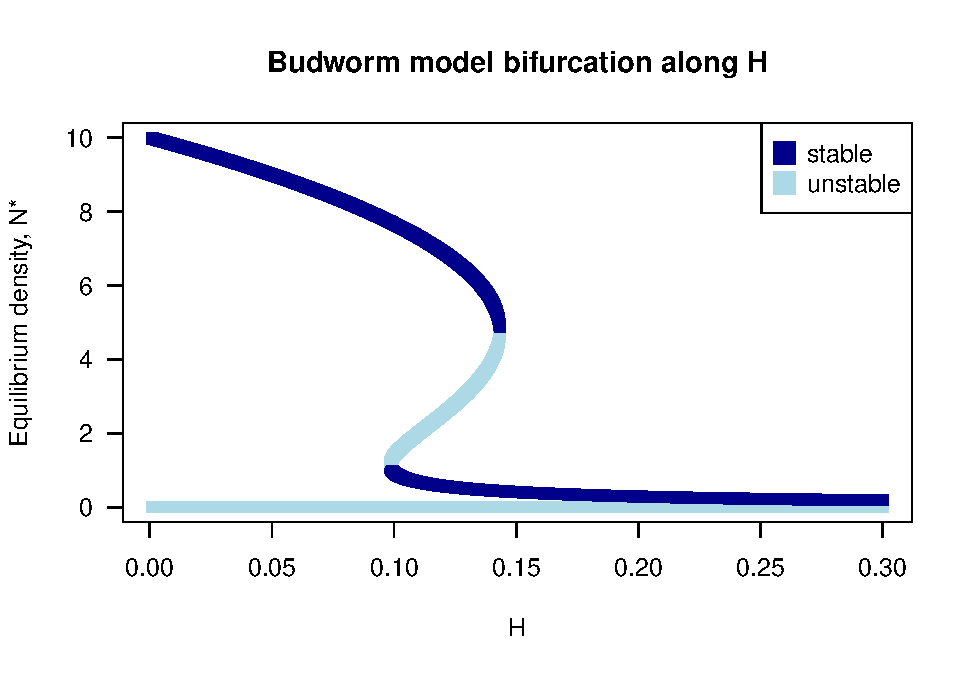
\includegraphics{bookdown-demo_files/figure-latex/unnamed-chunk-20-1.pdf}

\hypertarget{week-5---metapopulations-and-patch-occupancy-models}{%
\chapter*{Week 5 - Metapopulations and patch occupancy models}\label{week-5---metapopulations-and-patch-occupancy-models}}
\addcontentsline{toc}{chapter}{Week 5 - Metapopulations and patch occupancy models}

~~~~Plants can condition nearby soil microbial communities, which will in turn influence the performance of subsequent colonizing plants. The soil beneath plant communities are therefore a mosaic with different cultivation histories. Po-Ju wants to understand how plant demographic rates (i.e., colonization and mortality rate) and microbial dynamics (i.e., the conditioning and decay rate of microbial communities) affect the percentage of different soil types in natural forests. As a starting point, Po-Ju builds a one-species patch occupancy model to track the dynamics of different types of plant-soil combination.

~~~~In this model, he characterizes sites by their plant-soil microbe state, using the notation \(P_{ij}\) to indicate sites that are now occupied by plant species \(i\) but have soil microbes state \(j\). Here, as a single species model, \(i\) can be 0 or \(A\), representing uncolonized sites or sites colonized by plant \(A\), respectively. Similarly, \(j\) can be 0 or \(A\), indicating sites without recent plant conditioning history or sites conditioned by plant \(A\), respectively. In summary:

\begin{enumerate}
\def\labelenumi{\arabic{enumi}.}
\tightlist
\item
  \(P_{00}\) represents uncolonized and unconditioned sites
\item
  \(P_{A0}\) represents cites colonized by plant \(A\) but the soil is yet to be conditioned
\item
  \(P_{AA}\) represents plant \(A\) colonizing a site with plant-\(A\)-specific microbial community
\item
  \(P_{0A}\) represents sites that are currently unoccupied but have soil microbes that were associated with plant \(A\)
\end{enumerate}

At the landscape scale, \(P_{ij}\) represents the proportion of sites belonging to a particular plant-soil microbe state, and its dynamics, \(\frac {dP_{ij}}{dt}\), summarizes the processes of plant colonization and death. The transitions between different plant-soil microbe states can be described by the following figure.

Here, \(P_{00}\) can be colonized by plant \(A\) when propagules arrive (per capita rate \(r_{A}\)), transitioning the state from \(P_{00}\) to \(P_{A0}\). Plants may die, with rate \(m_{A}\), before conditioning the soil (i.e., transition from \(P_{A0}\) back to \(P_{00}\)), or may successfully condition the soil with rate \(c_{A}\) (i.e., transition from \(P_{A0}\) to \(P_{AA}\)). After plants within the state \(P_{AA}\) die, a site with microbial legacy is left behind, denoted as \(P_{0A}\). These empty sites can be recolonized (i.e., transition from \(P_{0A}\) back to \(P_{AA}\)) with rates affected by the microbial legacy effect, \(\alpha\). Finally, the microbial community within the soil may decay to unconditioned state with rate \(d_{A}\), transitioning the state from \(P_{0A}\) to \(P_{00}\).

~~~~In this lab, we are going to model the dynamics of this plant-soil system. We will start by converting the flow diagram into a set of differential equations and then solve them numerically using the package \texttt{deSolve}.

\begin{Shaded}
\begin{Highlighting}[]
\FunctionTok{library}\NormalTok{(deSolve)}
\FunctionTok{library}\NormalTok{(ggplot2)}
\FunctionTok{library}\NormalTok{(tidyr)}


\DocumentationTok{\#\#\# Model specification}
\NormalTok{PSF }\OtherTok{=} \ControlFlowTok{function}\NormalTok{(Time, State, Pars)\{}
  \FunctionTok{with}\NormalTok{(}\FunctionTok{as.list}\NormalTok{(}\FunctionTok{c}\NormalTok{(State, Pars)),\{}
\NormalTok{    dP00\_dt }\OtherTok{=} \SpecialCharTok{{-}}\NormalTok{ rA }\SpecialCharTok{*}\NormalTok{ (PA0 }\SpecialCharTok{+}\NormalTok{ PAA) }\SpecialCharTok{*}\NormalTok{ P00 }\SpecialCharTok{+}\NormalTok{ mA }\SpecialCharTok{*}\NormalTok{ PA0 }\SpecialCharTok{+}\NormalTok{ dA }\SpecialCharTok{*}\NormalTok{ P0A }
\NormalTok{    dPA0\_dt }\OtherTok{=}\NormalTok{ rA }\SpecialCharTok{*}\NormalTok{ (PA0 }\SpecialCharTok{+}\NormalTok{ PAA) }\SpecialCharTok{*}\NormalTok{ P00 }\SpecialCharTok{{-}}\NormalTok{ cA }\SpecialCharTok{*}\NormalTok{ PA0 }\SpecialCharTok{{-}}\NormalTok{ mA }\SpecialCharTok{*}\NormalTok{ PA0}
\NormalTok{    dPAA\_dt }\OtherTok{=}\NormalTok{ cA }\SpecialCharTok{*}\NormalTok{ PA0 }\SpecialCharTok{+}\NormalTok{ alpha }\SpecialCharTok{*}\NormalTok{ rA }\SpecialCharTok{*}\NormalTok{ (PA0 }\SpecialCharTok{+}\NormalTok{ PAA) }\SpecialCharTok{*}\NormalTok{ P0A }\SpecialCharTok{{-}}\NormalTok{ mA }\SpecialCharTok{*}\NormalTok{ PAA}
\NormalTok{    dP0A\_dt }\OtherTok{=}\NormalTok{ mA }\SpecialCharTok{*}\NormalTok{ PAA }\SpecialCharTok{{-}}\NormalTok{ alpha }\SpecialCharTok{*}\NormalTok{ rA }\SpecialCharTok{*}\NormalTok{ (PA0 }\SpecialCharTok{+}\NormalTok{ PAA) }\SpecialCharTok{*}\NormalTok{ P0A }\SpecialCharTok{{-}}\NormalTok{ dA }\SpecialCharTok{*}\NormalTok{ P0A}
    \FunctionTok{return}\NormalTok{(}\FunctionTok{list}\NormalTok{(}\FunctionTok{c}\NormalTok{(dP00\_dt, dPA0\_dt, dPAA\_dt, dP0A\_dt)))}
\NormalTok{  \})}
\NormalTok{\}}


\DocumentationTok{\#\#\#\# Set simulation parameters with the \textquotesingle{}quick simulation parameters\textquotesingle{}}
\NormalTok{pars }\OtherTok{=} \FunctionTok{c}\NormalTok{(}\AttributeTok{rA =} \FloatTok{0.5}\NormalTok{,}
         \AttributeTok{mA =} \FloatTok{0.1}\NormalTok{,}
         \AttributeTok{cA =} \FloatTok{0.5}\NormalTok{,}
         \AttributeTok{dA =} \FloatTok{0.4}\NormalTok{,}
         \AttributeTok{alpha =} \FloatTok{0.3}\NormalTok{)}


\DocumentationTok{\#\#\#\# Set initial condition and time steps}
\NormalTok{times }\OtherTok{=} \FunctionTok{seq}\NormalTok{(}\DecValTok{0}\NormalTok{, }\DecValTok{100}\NormalTok{, }\AttributeTok{by =} \FloatTok{0.1}\NormalTok{)}
\NormalTok{ini }\OtherTok{=} \FunctionTok{c}\NormalTok{(}\AttributeTok{P00 =} \FloatTok{0.75}\NormalTok{, }\AttributeTok{PA0 =} \FloatTok{0.1}\NormalTok{, }\AttributeTok{PAA =} \FloatTok{0.05}\NormalTok{, }\AttributeTok{P0A =} \FloatTok{0.1}\NormalTok{)}


\DocumentationTok{\#\#\#\# Run the simulation}
\NormalTok{pop\_size }\OtherTok{=} \FunctionTok{ode}\NormalTok{(}\AttributeTok{func =}\NormalTok{ PSF, }\AttributeTok{y =}\NormalTok{ ini, }\AttributeTok{parms =}\NormalTok{ pars, }\AttributeTok{times =}\NormalTok{ times)}


\DocumentationTok{\#\#\#\# Check if simulations reached stable point }
\FunctionTok{tail}\NormalTok{(pop\_size)}
\end{Highlighting}
\end{Shaded}

\begin{verbatim}
##          time       P00        PA0       PAA       P0A
##  [996,]  99.5 0.1634825 0.09738004 0.6174124 0.1217251
##  [997,]  99.6 0.1634825 0.09738004 0.6174124 0.1217251
##  [998,]  99.7 0.1634825 0.09738004 0.6174124 0.1217251
##  [999,]  99.8 0.1634825 0.09738004 0.6174124 0.1217251
## [1000,]  99.9 0.1634825 0.09738004 0.6174124 0.1217251
## [1001,] 100.0 0.1634825 0.09738004 0.6174124 0.1217251
\end{verbatim}

\begin{Shaded}
\begin{Highlighting}[]
\FunctionTok{rowSums}\NormalTok{(}\FunctionTok{tail}\NormalTok{(pop\_size[, }\SpecialCharTok{{-}}\DecValTok{1}\NormalTok{]))}
\end{Highlighting}
\end{Shaded}

\begin{verbatim}
##  [996,]  [997,]  [998,]  [999,] [1000,] [1001,] 
##       1       1       1       1       1       1
\end{verbatim}

~~~~After checking the outcomes of our numerical simulation, we can visualize the system dynamics through time, using any method you prefer. The following are some examples:

Visualization of the system dynamics through time using function \texttt{matplot}.

\begin{Shaded}
\begin{Highlighting}[]
\DocumentationTok{\#\#\#\# Plot (matplot)}
\FunctionTok{matplot}\NormalTok{(}\AttributeTok{x =}\NormalTok{ pop\_size[, }\DecValTok{1}\NormalTok{], }\AttributeTok{y =}\NormalTok{ pop\_size[, }\DecValTok{2}\SpecialCharTok{:}\DecValTok{5}\NormalTok{], }\AttributeTok{type =} \StringTok{"l"}\NormalTok{)}
\end{Highlighting}
\end{Shaded}

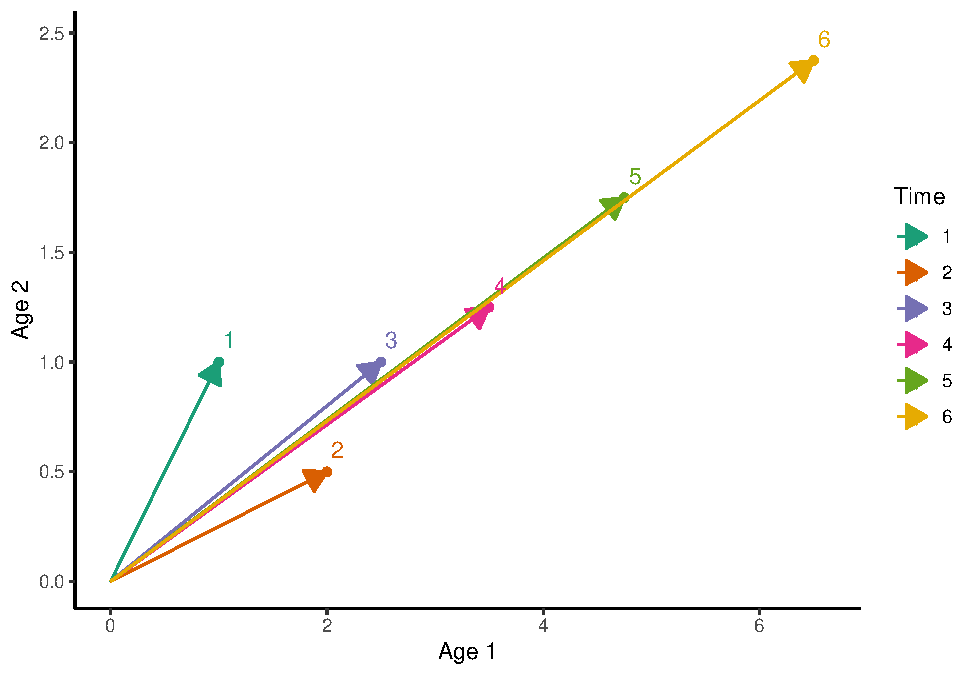
\includegraphics{bookdown-demo_files/figure-latex/unnamed-chunk-22-1.pdf}

Visualization of the system dynamics through time using base R, with axis labels and given line colors.

\begin{Shaded}
\begin{Highlighting}[]
\DocumentationTok{\#\#\#\# Plot (base R)}
\FunctionTok{plot}\NormalTok{(}\AttributeTok{x =} \FunctionTok{range}\NormalTok{(times), }\AttributeTok{y =} \FunctionTok{c}\NormalTok{(}\DecValTok{0}\NormalTok{,}\DecValTok{1}\NormalTok{), }\AttributeTok{type =} \StringTok{"n"}\NormalTok{, }\AttributeTok{xlab =} \StringTok{"Time"}\NormalTok{, }\AttributeTok{ylab =} \StringTok{"Proportion"}\NormalTok{)}
\FunctionTok{lines}\NormalTok{(P00 }\SpecialCharTok{\textasciitilde{}}\NormalTok{ time, }\AttributeTok{data =}\NormalTok{ pop\_size, }\AttributeTok{col =} \StringTok{"black"}\NormalTok{)}
\FunctionTok{lines}\NormalTok{(PA0 }\SpecialCharTok{\textasciitilde{}}\NormalTok{ time, }\AttributeTok{data =}\NormalTok{ pop\_size, }\AttributeTok{col =} \StringTok{"blue"}\NormalTok{)}
\FunctionTok{lines}\NormalTok{(PAA }\SpecialCharTok{\textasciitilde{}}\NormalTok{ time, }\AttributeTok{data =}\NormalTok{ pop\_size, }\AttributeTok{col =} \StringTok{"purple"}\NormalTok{)}
\FunctionTok{lines}\NormalTok{(P0A }\SpecialCharTok{\textasciitilde{}}\NormalTok{ time, }\AttributeTok{data =}\NormalTok{ pop\_size, }\AttributeTok{col =} \StringTok{"red"}\NormalTok{)}
\FunctionTok{legend}\NormalTok{(}\StringTok{"topleft"}\NormalTok{, }
       \AttributeTok{legend =} \FunctionTok{c}\NormalTok{(}\StringTok{"P00"}\NormalTok{, }\StringTok{"PA0"}\NormalTok{, }\StringTok{"PAA"}\NormalTok{, }\StringTok{"P0A"}\NormalTok{), }
       \AttributeTok{col =} \FunctionTok{c}\NormalTok{(}\StringTok{"black"}\NormalTok{, }\StringTok{"blue"}\NormalTok{, }\StringTok{"purple"}\NormalTok{, }\StringTok{"red"}\NormalTok{), }\AttributeTok{lty =} \DecValTok{1}\NormalTok{, }\AttributeTok{bty =} \StringTok{"n"}\NormalTok{)}
\end{Highlighting}
\end{Shaded}

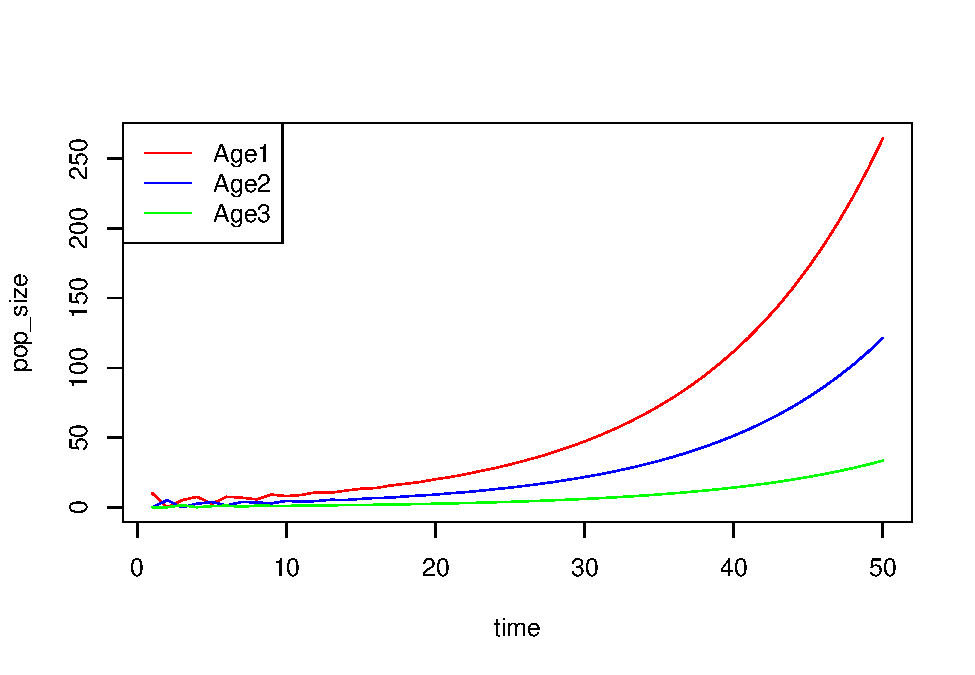
\includegraphics{bookdown-demo_files/figure-latex/unnamed-chunk-23-1.pdf}

Data organization using package \texttt{tidyverse} and visualization of the system dynamics through time using package \texttt{ggplot2}.

\begin{Shaded}
\begin{Highlighting}[]
\DocumentationTok{\#\#\# ggplot course website version}
\NormalTok{pop\_size }\SpecialCharTok{\%\textgreater{}\%}
  \FunctionTok{as.data.frame}\NormalTok{() }\SpecialCharTok{\%\textgreater{}\%}
  \FunctionTok{gather}\NormalTok{(}\AttributeTok{key =} \StringTok{"Patch"}\NormalTok{, }\AttributeTok{value =} \StringTok{"Proportion"}\NormalTok{, }\SpecialCharTok{{-}}\NormalTok{time) }\SpecialCharTok{\%\textgreater{}\%}
  \FunctionTok{ggplot}\NormalTok{(}\FunctionTok{aes}\NormalTok{(}\AttributeTok{x =}\NormalTok{ time, }\AttributeTok{y =}\NormalTok{ Proportion, }\AttributeTok{color =}\NormalTok{ Patch)) }\SpecialCharTok{+}
  \FunctionTok{geom\_line}\NormalTok{(}\AttributeTok{linewidth =} \FloatTok{1.5}\NormalTok{)}
\end{Highlighting}
\end{Shaded}

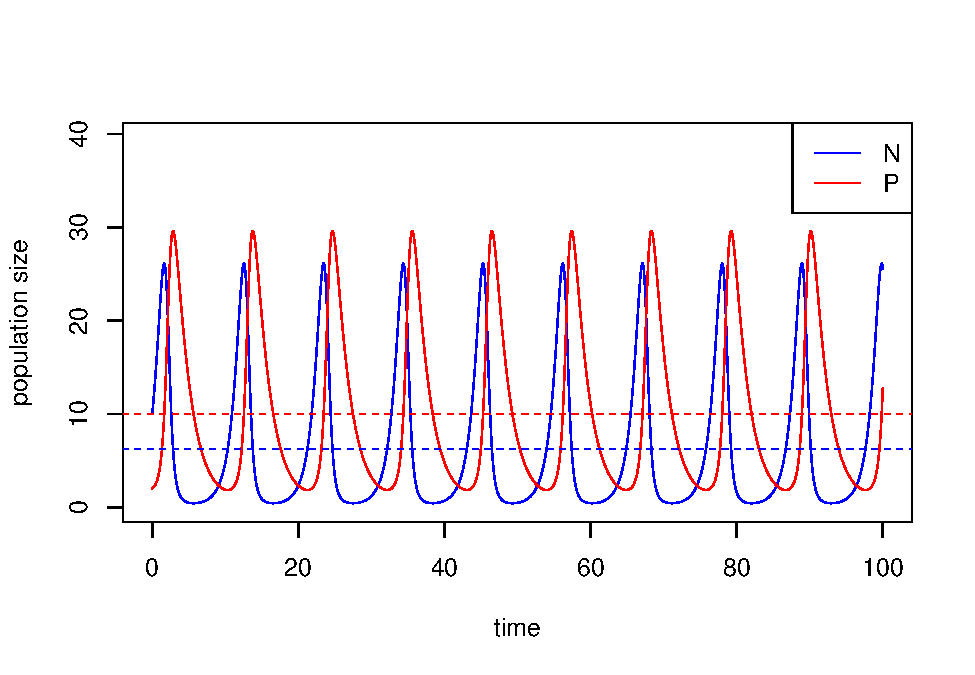
\includegraphics{bookdown-demo_files/figure-latex/unnamed-chunk-24-1.pdf}

~~~~Now we see that the system would eventually be stable, we can jump through the time series and directly take the final equilibrium point (assuming the selected simulation length works for different parameter values). Our next step is to modify the target parameter related to our research question and study their resulting outcome. For example, we want to see how the final fate of this system would change under different decay rates of the conditioned microbial effect (i.e., d\_\{A\}, the transitioning from P\_\{0A\} to uncolonized and unconditioned soil P\_\{00\}). We can efficiently vary the target parameter using a for-loop to run the simulation under different decay rates.

Using for loop to run the simulation under different decay rates (\(d_{A}\)).

\begin{Shaded}
\begin{Highlighting}[]
\DocumentationTok{\#\#\# For{-}loop over different parameter values }
\DocumentationTok{\#\#\# Parameter range and saving space setup}
\NormalTok{dA\_seq }\OtherTok{\textless{}{-}} \FunctionTok{seq}\NormalTok{(}\AttributeTok{from =} \FloatTok{0.1}\NormalTok{, }\AttributeTok{to =} \FloatTok{0.8}\NormalTok{, }\AttributeTok{by =} \FloatTok{0.1}\NormalTok{)}
\NormalTok{Data }\OtherTok{\textless{}{-}} \FunctionTok{as.data.frame}\NormalTok{(}\FunctionTok{matrix}\NormalTok{(}\DecValTok{0}\NormalTok{, }\AttributeTok{nrow =} \FunctionTok{length}\NormalTok{(dA\_seq), }\AttributeTok{ncol =} \DecValTok{6}\NormalTok{))}
\FunctionTok{names}\NormalTok{(Data) }\OtherTok{\textless{}{-}} \FunctionTok{c}\NormalTok{(}\StringTok{"dA"}\NormalTok{, }\StringTok{"time"}\NormalTok{, }\StringTok{"P00"}\NormalTok{, }\StringTok{"PA0"}\NormalTok{, }\StringTok{"PAA"}\NormalTok{, }\StringTok{"P0A"}\NormalTok{)}
\NormalTok{Data[, }\DecValTok{1}\NormalTok{] }\OtherTok{\textless{}{-}}\NormalTok{ dA\_seq}

\DocumentationTok{\#\#\# Use for loop to change the parameter every time}
\ControlFlowTok{for}\NormalTok{(i }\ControlFlowTok{in} \DecValTok{1}\SpecialCharTok{:}\FunctionTok{length}\NormalTok{(dA\_seq))\{}
  
  \CommentTok{\# Set simulation parameters}
\NormalTok{  pars\_new }\OtherTok{\textless{}{-}} \FunctionTok{c}\NormalTok{(}\AttributeTok{rA =} \FloatTok{0.5}\NormalTok{, }\AttributeTok{mA =} \FloatTok{0.1}\NormalTok{, }\AttributeTok{cA =} \FloatTok{0.5}\NormalTok{, }\AttributeTok{dA =}\NormalTok{ dA\_seq[i], }\AttributeTok{alpha =} \FloatTok{0.3}\NormalTok{)}
  
  \CommentTok{\# Simulate}
\NormalTok{  pop\_size\_new }\OtherTok{\textless{}{-}} \FunctionTok{ode}\NormalTok{(}\AttributeTok{func =}\NormalTok{ PSF, }\AttributeTok{y =}\NormalTok{ ini, }\AttributeTok{parms =}\NormalTok{ pars\_new, }\AttributeTok{times =}\NormalTok{ times)}
  
  \CommentTok{\# Save results}
\NormalTok{  Data[i, }\FunctionTok{c}\NormalTok{(}\DecValTok{2}\SpecialCharTok{:}\DecValTok{6}\NormalTok{)] }\OtherTok{\textless{}{-}}\NormalTok{ pop\_size\_new[}\FunctionTok{length}\NormalTok{(times), ]}
\NormalTok{\}}
\end{Highlighting}
\end{Shaded}

Visualization of the stable state under different decay rates (\(d_{A}\)) using base R, with axis labels and given line colors. Does the pattern match your intuition?

\begin{Shaded}
\begin{Highlighting}[]
\DocumentationTok{\#\#\# Plot resulting equilibrium against different dA  }
\FunctionTok{plot}\NormalTok{(}\AttributeTok{x =} \FunctionTok{range}\NormalTok{(dA\_seq), }\AttributeTok{y =} \FunctionTok{c}\NormalTok{(}\DecValTok{0}\NormalTok{,}\DecValTok{1}\NormalTok{), }\AttributeTok{type =} \StringTok{"n"}\NormalTok{, }
     \AttributeTok{xlab =} \StringTok{"Decay rate of conditioned soil"}\NormalTok{, }
     \AttributeTok{ylab =} \StringTok{"Equilibrium proportion"}\NormalTok{)}
\FunctionTok{lines}\NormalTok{(P00 }\SpecialCharTok{\textasciitilde{}}\NormalTok{ dA, }\AttributeTok{data =}\NormalTok{ Data, }\AttributeTok{col =} \StringTok{"black"}\NormalTok{)}
\FunctionTok{lines}\NormalTok{(PA0 }\SpecialCharTok{\textasciitilde{}}\NormalTok{ dA, }\AttributeTok{data =}\NormalTok{ Data, }\AttributeTok{col =} \StringTok{"blue"}\NormalTok{)}
\FunctionTok{lines}\NormalTok{(PAA }\SpecialCharTok{\textasciitilde{}}\NormalTok{ dA, }\AttributeTok{data =}\NormalTok{ Data, }\AttributeTok{col =} \StringTok{"purple"}\NormalTok{)}
\FunctionTok{lines}\NormalTok{(P0A }\SpecialCharTok{\textasciitilde{}}\NormalTok{ dA, }\AttributeTok{data =}\NormalTok{ Data, }\AttributeTok{col =} \StringTok{"red"}\NormalTok{)}
\FunctionTok{legend}\NormalTok{(}\StringTok{"topleft"}\NormalTok{, }
       \AttributeTok{legend =} \FunctionTok{c}\NormalTok{(}\StringTok{"P00"}\NormalTok{, }\StringTok{"PA0"}\NormalTok{, }\StringTok{"PAA"}\NormalTok{, }\StringTok{"P0A"}\NormalTok{), }
       \AttributeTok{col =} \FunctionTok{c}\NormalTok{(}\StringTok{"black"}\NormalTok{, }\StringTok{"blue"}\NormalTok{, }\StringTok{"purple"}\NormalTok{, }\StringTok{"red"}\NormalTok{), }\AttributeTok{lty =} \DecValTok{1}\NormalTok{, }\AttributeTok{bty =} \StringTok{"n"}\NormalTok{)}
\end{Highlighting}
\end{Shaded}

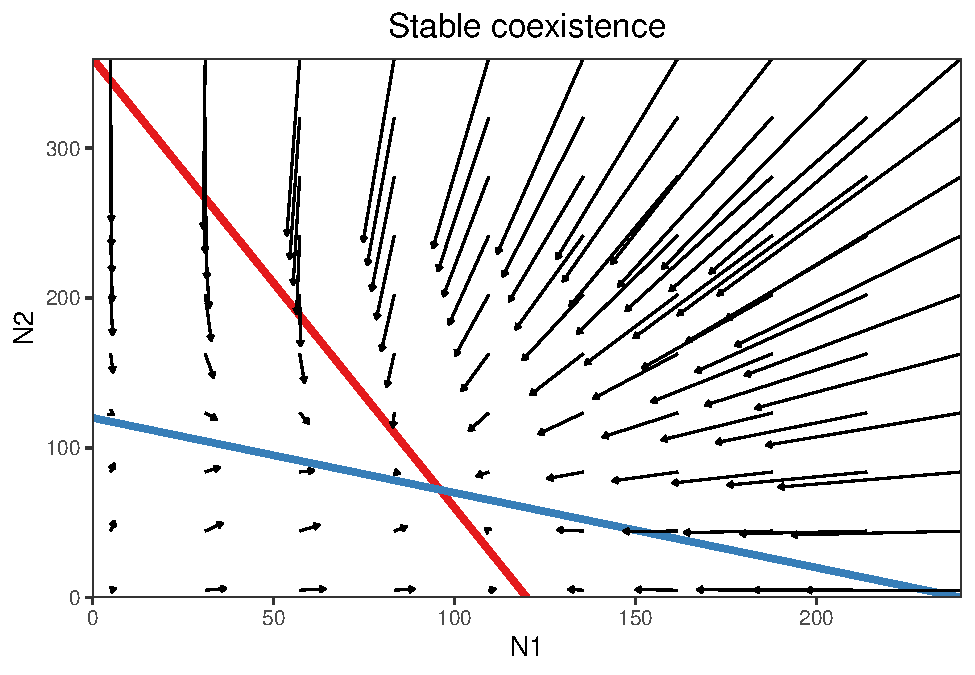
\includegraphics{bookdown-demo_files/figure-latex/unnamed-chunk-26-1.pdf}
Visualization of the stable state under different decay rates (\(d_{A}\)) using package \texttt{ggplot2}.

\begin{Shaded}
\begin{Highlighting}[]
\DocumentationTok{\#\#\# ggplot course website version}
\NormalTok{Data }\SpecialCharTok{\%\textgreater{}\%}
  \FunctionTok{as.data.frame}\NormalTok{() }\SpecialCharTok{\%\textgreater{}\%}
  \FunctionTok{gather}\NormalTok{(}\AttributeTok{key =} \StringTok{"Patch"}\NormalTok{, }\AttributeTok{value =} \StringTok{"Proportion"}\NormalTok{,}\SpecialCharTok{{-}}\NormalTok{dA, }\SpecialCharTok{{-}}\NormalTok{time) }\SpecialCharTok{\%\textgreater{}\%}
  \FunctionTok{ggplot}\NormalTok{(}\FunctionTok{aes}\NormalTok{(}\AttributeTok{x =}\NormalTok{ dA, }\AttributeTok{y =}\NormalTok{ Proportion, }\AttributeTok{color =}\NormalTok{ Patch)) }\SpecialCharTok{+}
  \FunctionTok{geom\_line}\NormalTok{(}\AttributeTok{linewidth =} \FloatTok{1.5}\NormalTok{)}
\end{Highlighting}
\end{Shaded}

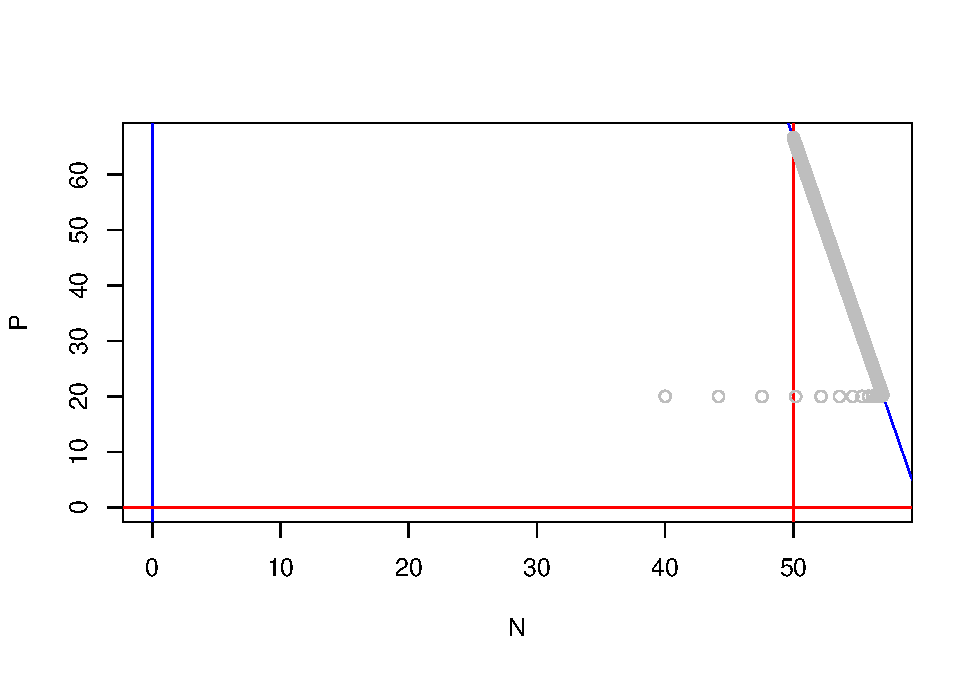
\includegraphics{bookdown-demo_files/figure-latex/unnamed-chunk-27-1.pdf}

\hypertarget{week-6---harvesting-and-bifurcation}{%
\chapter*{Week 6 - Harvesting and bifurcation}\label{week-6---harvesting-and-bifurcation}}
\addcontentsline{toc}{chapter}{Week 6 - Harvesting and bifurcation}

In this lab section, we're going to analyze the budworm population
dynamic model from \href{https://doi.org/10.2307/3939}{\textbf{Ludwig et al.,
1978}}.

\textbf{Part 1 - Stability of the budworm model}

In part 1 we're going to visualize the stability of the budworm model,
by plotting the differential equation. We will plot the the differential
equation with different initial, which we will see that the number and stability of equilibrium changes when parameter changes.

\[
\dfrac{dN}{dt} = rN(1 - \dfrac{N}{K}) - \dfrac{HN^2}{A^2 + N^2}
\]

\begin{Shaded}
\begin{Highlighting}[]
\DocumentationTok{\#\#\#\# Plotting the functional form for different parameters}
\DocumentationTok{\#\#\#\# Parameter setting}
\NormalTok{r }\OtherTok{\textless{}{-}} \FloatTok{0.055}\NormalTok{; K }\OtherTok{\textless{}{-}} \DecValTok{10}\NormalTok{; H }\OtherTok{\textless{}{-}} \FloatTok{0.1}\NormalTok{; A }\OtherTok{\textless{}{-}} \DecValTok{1}

\DocumentationTok{\#\#\#\# Visualize the whole dN/dt with different H}
\NormalTok{N.vec }\OtherTok{\textless{}{-}} \FunctionTok{seq}\NormalTok{(}\AttributeTok{from =} \DecValTok{0}\NormalTok{, }\AttributeTok{to =} \DecValTok{10}\NormalTok{, }\AttributeTok{length =} \DecValTok{500}\NormalTok{)}
\NormalTok{H.breaks }\OtherTok{\textless{}{-}} \FunctionTok{c}\NormalTok{(}\FloatTok{0.05}\NormalTok{, }\FloatTok{0.12}\NormalTok{, }\FloatTok{0.20}\NormalTok{)}
\NormalTok{dat }\OtherTok{\textless{}{-}} \FunctionTok{outer}\NormalTok{(}\AttributeTok{X =}\NormalTok{ N.vec, }\AttributeTok{Y =}\NormalTok{ H.breaks,}
             \ControlFlowTok{function}\NormalTok{(N, H)\{r }\SpecialCharTok{*}\NormalTok{ N }\SpecialCharTok{*}\NormalTok{ (}\DecValTok{1} \SpecialCharTok{{-}}\NormalTok{ N }\SpecialCharTok{/}\NormalTok{ K) }\SpecialCharTok{{-}}\NormalTok{ (H }\SpecialCharTok{*}\NormalTok{ N}\SpecialCharTok{\^{}}\DecValTok{2} \SpecialCharTok{/}\NormalTok{ (A}\SpecialCharTok{\^{}}\DecValTok{2} \SpecialCharTok{+}\NormalTok{ N}\SpecialCharTok{\^{}}\DecValTok{2}\NormalTok{))\})}
\FunctionTok{matplot}\NormalTok{(}\AttributeTok{x =}\NormalTok{ N.vec, }\AttributeTok{y =}\NormalTok{ dat, }\AttributeTok{type =} \StringTok{"l"}\NormalTok{, }
        \AttributeTok{xlab =} \StringTok{"N"}\NormalTok{, }\AttributeTok{ylab =} \StringTok{"dN/dt"}\NormalTok{, }\AttributeTok{col =} \StringTok{"blue"}\NormalTok{, }\AttributeTok{lwd =} \DecValTok{2}\NormalTok{, }\AttributeTok{las =} \DecValTok{1}\NormalTok{)}
\FunctionTok{abline}\NormalTok{(}\AttributeTok{h =} \DecValTok{0}\NormalTok{)}
\FunctionTok{legend}\NormalTok{(}\StringTok{"bottomleft"}\NormalTok{, }\AttributeTok{legend =}\NormalTok{ H.breaks, }\AttributeTok{title =} \StringTok{"H"}\NormalTok{, }\AttributeTok{col =} \StringTok{"blue"}\NormalTok{, }\AttributeTok{lty=}\DecValTok{1}\SpecialCharTok{:}\DecValTok{3}\NormalTok{, }\AttributeTok{lwd =} \DecValTok{2}\NormalTok{)}
\end{Highlighting}
\end{Shaded}

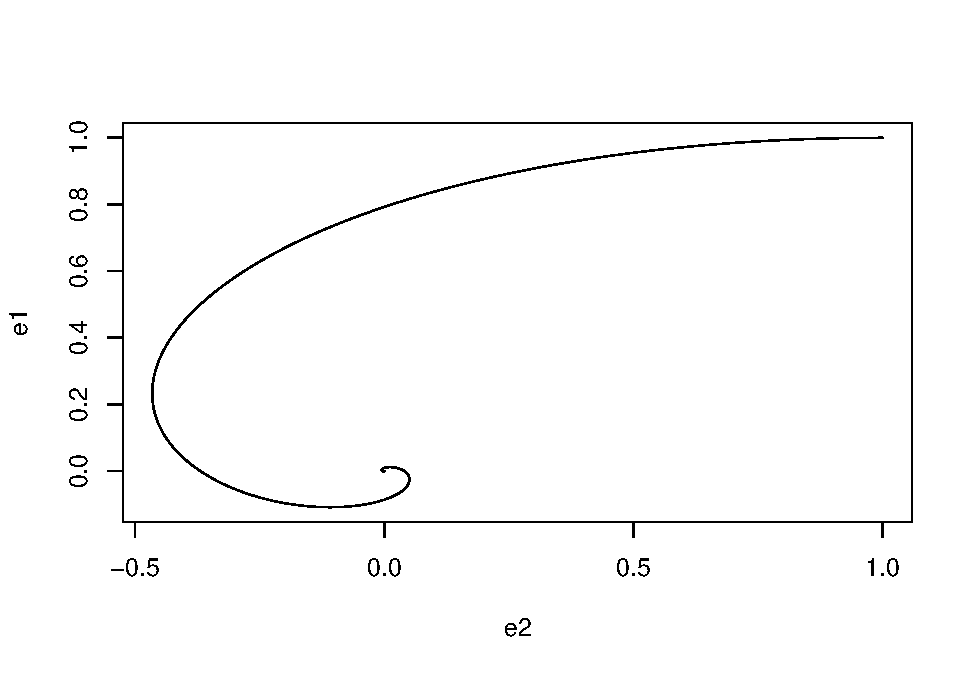
\includegraphics{bookdown-demo_files/figure-latex/unnamed-chunk-28-1.pdf}

Second, we're going to plot \(harvest\) rate against \(N\) with
separate components of \(dN/Ndt\), which the blue line is
\[
\dfrac{HN}{A^2 + N^2}
\]
with different \(H\), the red line is,
\[
r(1 - \dfrac{N}{K})
\]
and the points that blue line and red line crosses are the equilibrium points.

\begin{Shaded}
\begin{Highlighting}[]
\DocumentationTok{\#\#\#\# Visualize separate components of dN/Ndt with different H}
\NormalTok{N.vec }\OtherTok{\textless{}{-}} \FunctionTok{seq}\NormalTok{(}\AttributeTok{from =} \DecValTok{0}\NormalTok{, }\AttributeTok{to =} \DecValTok{10}\NormalTok{, }\AttributeTok{length =} \DecValTok{500}\NormalTok{)}
\NormalTok{H.breaks }\OtherTok{\textless{}{-}} \FunctionTok{c}\NormalTok{(}\FloatTok{0.05}\NormalTok{, }\FloatTok{0.12}\NormalTok{, }\FloatTok{0.20}\NormalTok{)}
\NormalTok{dat.growth }\OtherTok{\textless{}{-}} \FunctionTok{outer}\NormalTok{(}\AttributeTok{X =}\NormalTok{ N.vec, }\AttributeTok{Y =}\NormalTok{ H.breaks,}
                    \ControlFlowTok{function}\NormalTok{(N, H)\{H }\SpecialCharTok{*}\NormalTok{ N }\SpecialCharTok{/}\NormalTok{ (A}\SpecialCharTok{\^{}}\DecValTok{2} \SpecialCharTok{+}\NormalTok{ N}\SpecialCharTok{\^{}}\DecValTok{2}\NormalTok{)\}) }\CommentTok{\# Note notation change}
\FunctionTok{matplot}\NormalTok{(}\AttributeTok{x =}\NormalTok{ N.vec, }\AttributeTok{y =}\NormalTok{ dat.growth, }\AttributeTok{type =} \StringTok{"l"}\NormalTok{, }\AttributeTok{ylim =} \FunctionTok{c}\NormalTok{(}\DecValTok{0}\NormalTok{, }\FloatTok{0.10}\NormalTok{), }\AttributeTok{las =} \DecValTok{1}\NormalTok{, }
        \AttributeTok{xlab =} \StringTok{"N"}\NormalTok{, }\AttributeTok{ylab =} \StringTok{"growth / harvest rate"}\NormalTok{, }\AttributeTok{col =} \StringTok{"blue"}\NormalTok{, }\AttributeTok{lwd =} \DecValTok{2}\NormalTok{)}
\FunctionTok{curve}\NormalTok{(r }\SpecialCharTok{*}\NormalTok{ (}\DecValTok{1} \SpecialCharTok{{-}}\NormalTok{ x}\SpecialCharTok{/}\NormalTok{K), }\AttributeTok{add =}\NormalTok{ T, }\AttributeTok{col =} \StringTok{"red"}\NormalTok{, }\AttributeTok{lwd =} \DecValTok{2}\NormalTok{) }\CommentTok{\# Just curve since its the same line, and note variable notation change}
\FunctionTok{abline}\NormalTok{(}\AttributeTok{h =} \DecValTok{0}\NormalTok{)}
\FunctionTok{legend}\NormalTok{(}\StringTok{"topright"}\NormalTok{, }\AttributeTok{legend =}\NormalTok{ H.breaks, }\AttributeTok{title =} \StringTok{"H"}\NormalTok{, }\AttributeTok{col =} \StringTok{"blue"}\NormalTok{, }\AttributeTok{lty=}\DecValTok{1}\SpecialCharTok{:}\DecValTok{3}\NormalTok{, }\AttributeTok{lwd =} \DecValTok{2}\NormalTok{)}
\end{Highlighting}
\end{Shaded}

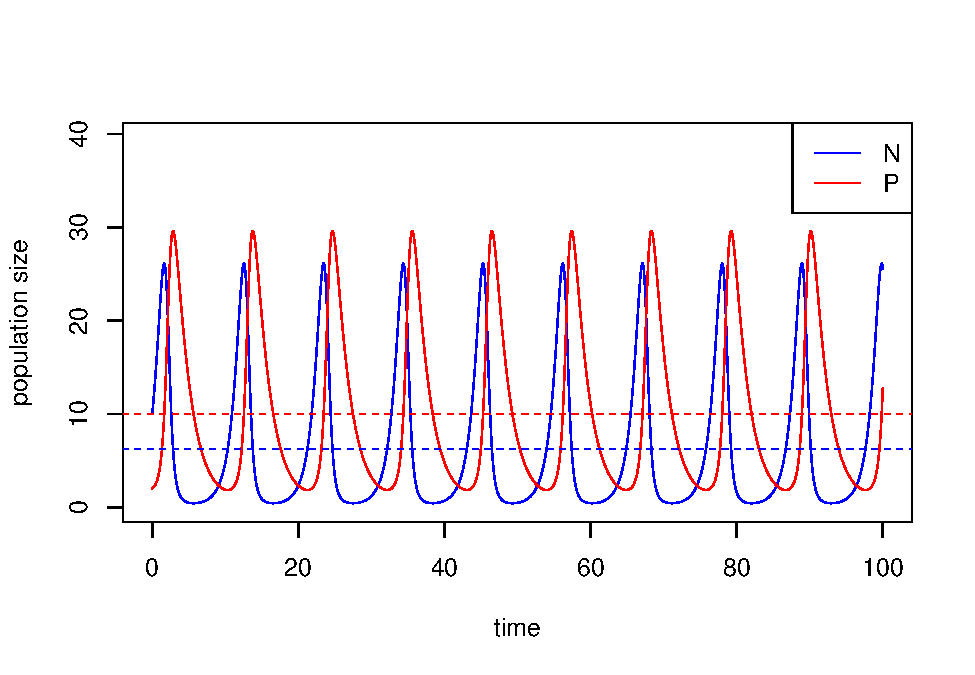
\includegraphics{bookdown-demo_files/figure-latex/unnamed-chunk-29-1.pdf}

\textbf{Part 2 - Use \texttt{rootSolve} function \texttt{gradient} and \texttt{uniroot.all}, to solve stability of budworm model}

\begin{Shaded}
\begin{Highlighting}[]
\DocumentationTok{\#\#\#\# Stability of the budworm model, as a function of its parameters}
\DocumentationTok{\#\#\#\# Using "rootSolve" function "gradient" and "uniroot.all"}
\DocumentationTok{\#\#\#\# Works best for simple models and those with known solutions}
\DocumentationTok{\#\#\#\#\#\#\#\#\#\#\#\#\#\#\#\#\#\#\#\#\#\#\#\#\#\#\#\#\#\#\#\#\#\#\#\#\#\#\#\#\#\#\#\#\#\#\#\#\#\#\#\#\#\#\#\#\#\#\#\#\#\#\#\#\#\#\#\#\#\#\#\#\#\#\#\#\#\#\#\#\#\#\#\#\#\#\#\#\#\#\#\#\#\#\#\#\#\#\#\#\#\#\#\#\#\#\#\#\#\#\#\#\#\#\#\#\#\#\#\#}
\FunctionTok{library}\NormalTok{(rootSolve)}
\DocumentationTok{\#\#\#\# Parameter setting}
\NormalTok{r }\OtherTok{\textless{}{-}} \FloatTok{0.055}\NormalTok{; K }\OtherTok{\textless{}{-}} \DecValTok{10}\NormalTok{; H }\OtherTok{\textless{}{-}} \FloatTok{0.1}\NormalTok{; A }\OtherTok{\textless{}{-}} \DecValTok{1}

\DocumentationTok{\#\#\#\# Spruce budworm model for rootSolve}
\NormalTok{Budworm }\OtherTok{\textless{}{-}} \ControlFlowTok{function}\NormalTok{(N, }\AttributeTok{H =} \FloatTok{0.1}\NormalTok{)\{}
\NormalTok{  r }\SpecialCharTok{*}\NormalTok{ N }\SpecialCharTok{*}\NormalTok{ (}\DecValTok{1} \SpecialCharTok{{-}}\NormalTok{ N }\SpecialCharTok{/}\NormalTok{ K) }\SpecialCharTok{{-}}\NormalTok{ (H }\SpecialCharTok{*}\NormalTok{ N}\SpecialCharTok{\^{}}\DecValTok{2} \SpecialCharTok{/}\NormalTok{ (A}\SpecialCharTok{\^{}}\DecValTok{2} \SpecialCharTok{+}\NormalTok{ N}\SpecialCharTok{\^{}}\DecValTok{2}\NormalTok{))}
\NormalTok{\}}

\DocumentationTok{\#\#\#\# Function of root stability}
\NormalTok{Stability }\OtherTok{\textless{}{-}} \ControlFlowTok{function}\NormalTok{(}\AttributeTok{H.value =} \FloatTok{0.1}\NormalTok{)\{}
\NormalTok{  equilibrium }\OtherTok{\textless{}{-}} \FunctionTok{uniroot.all}\NormalTok{(}\AttributeTok{f =}\NormalTok{ Budworm, }\AttributeTok{interval =} \FunctionTok{c}\NormalTok{(}\DecValTok{0}\NormalTok{, K), }\AttributeTok{H =}\NormalTok{ H.value) }\CommentTok{\# finds all roots}
\NormalTok{  lambda }\OtherTok{\textless{}{-}} \FunctionTok{vector}\NormalTok{(}\AttributeTok{mode =} \StringTok{"numeric"}\NormalTok{, }\AttributeTok{length =} \FunctionTok{length}\NormalTok{(equilibrium))}
  \ControlFlowTok{for}\NormalTok{(i }\ControlFlowTok{in} \DecValTok{1}\SpecialCharTok{:}\FunctionTok{length}\NormalTok{(equilibrium))\{}
\NormalTok{    lambda[i] }\OtherTok{\textless{}{-}} \FunctionTok{sign}\NormalTok{(}\FunctionTok{gradient}\NormalTok{(}\AttributeTok{f =}\NormalTok{ Budworm, }\AttributeTok{x =}\NormalTok{ equilibrium[i], }\AttributeTok{H =}\NormalTok{ H.value))}
\NormalTok{  \}}
  \FunctionTok{return}\NormalTok{(}\FunctionTok{list}\NormalTok{(}\AttributeTok{Equilibrium =}\NormalTok{ equilibrium,}
              \AttributeTok{Lambda =}\NormalTok{ lambda))}
\NormalTok{\}}

\DocumentationTok{\#\#\#\# Bifurcation diagram for H}
\NormalTok{H.vec }\OtherTok{\textless{}{-}} \FunctionTok{seq}\NormalTok{(}\FloatTok{0.001}\NormalTok{, }\FloatTok{0.3}\NormalTok{, }\AttributeTok{by =} \FloatTok{0.0001}\NormalTok{)}

\DocumentationTok{\#\# Create plotting frame}
\FunctionTok{plot}\NormalTok{(}\DecValTok{0}\NormalTok{, }\AttributeTok{xlim =} \FunctionTok{range}\NormalTok{(H.vec), }\AttributeTok{ylim =} \FunctionTok{c}\NormalTok{(}\DecValTok{0}\NormalTok{, }\DecValTok{10}\NormalTok{), }\AttributeTok{type =} \StringTok{"n"}\NormalTok{, }\AttributeTok{las =} \DecValTok{1}\NormalTok{,}
     \AttributeTok{xlab =} \StringTok{"H"}\NormalTok{, }\AttributeTok{ylab =} \StringTok{"Equilibrium density, N*"}\NormalTok{, }\AttributeTok{main =} \StringTok{"Budworm model bifurcation along H"}\NormalTok{)}
\FunctionTok{legend}\NormalTok{(}\StringTok{"topright"}\NormalTok{, }\AttributeTok{pch =} \DecValTok{15}\NormalTok{, }\AttributeTok{pt.cex =} \DecValTok{2}\NormalTok{, }\FunctionTok{c}\NormalTok{(}\StringTok{"stable"}\NormalTok{, }\StringTok{"unstable"}\NormalTok{),}
       \AttributeTok{col =} \FunctionTok{c}\NormalTok{(}\StringTok{"darkblue"}\NormalTok{, }\StringTok{"lightblue"}\NormalTok{))}

\DocumentationTok{\#\# Calculate number of roots and stability across range of H}
\ControlFlowTok{for}\NormalTok{(H }\ControlFlowTok{in}\NormalTok{ H.vec)\{}
\NormalTok{  temp }\OtherTok{\textless{}{-}} \FunctionTok{Stability}\NormalTok{(}\AttributeTok{H.value =}\NormalTok{ H)}
  \FunctionTok{points}\NormalTok{(}\AttributeTok{x =} \FunctionTok{rep}\NormalTok{(H, }\FunctionTok{length}\NormalTok{(temp}\SpecialCharTok{$}\NormalTok{Equilibrium)),}
         \AttributeTok{y =}\NormalTok{ temp}\SpecialCharTok{$}\NormalTok{Equilibrium,}
         \AttributeTok{pch =} \DecValTok{15}\NormalTok{, }\AttributeTok{col =} \FunctionTok{ifelse}\NormalTok{(temp}\SpecialCharTok{$}\NormalTok{Lambda }\SpecialCharTok{==} \SpecialCharTok{{-}}\DecValTok{1}\NormalTok{, }\StringTok{"darkblue"}\NormalTok{, }\StringTok{"lightblue"}\NormalTok{))}
\NormalTok{\}}
\end{Highlighting}
\end{Shaded}

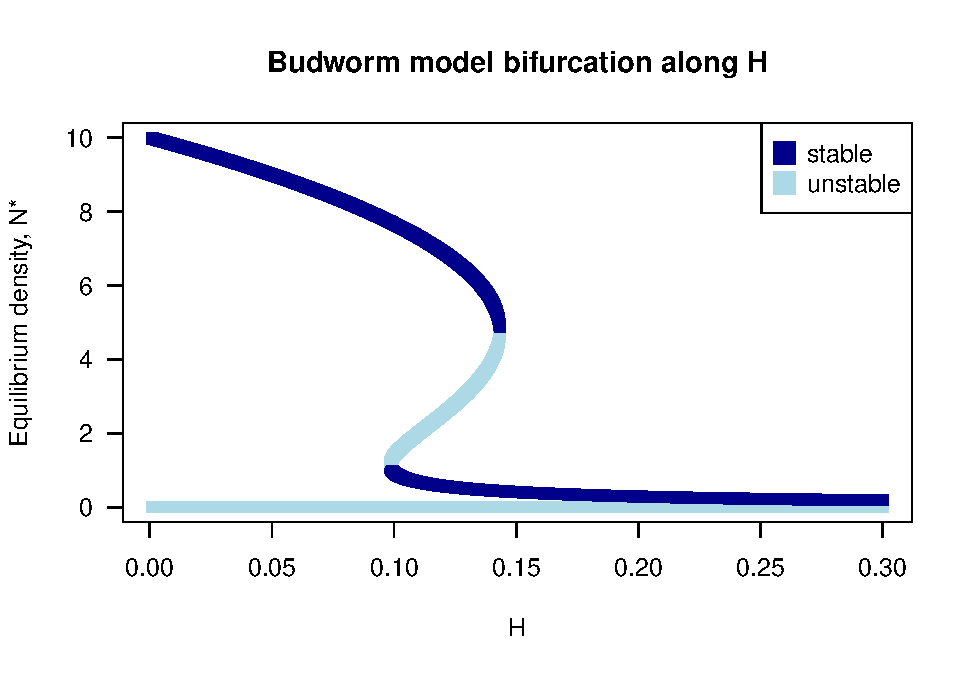
\includegraphics{bookdown-demo_files/figure-latex/unnamed-chunk-30-1.pdf}

Take a look a this
\href{https://www.math.ksu.edu/~albin/teaching/math340_fall2018/slides/03_bifurcations.html}{\textbf{website}} if you're interested in more details of bifurcation.

\textbf{Extra materials}
\textbf{Using \texttt{deSolve} function \texttt{ode} to brute-force stable solution}

Here we're going to use \texttt{deSolve} to solve the budworm model,

\begin{Shaded}
\begin{Highlighting}[]
\DocumentationTok{\#\#\#\# Budworm model for deSolve}

\FunctionTok{library}\NormalTok{(deSolve)}

\NormalTok{BudwormODE }\OtherTok{\textless{}{-}} \ControlFlowTok{function}\NormalTok{(times, state, parms) \{}
  \FunctionTok{with}\NormalTok{(}\FunctionTok{as.list}\NormalTok{(}\FunctionTok{c}\NormalTok{(state, parms)), \{}
\NormalTok{    dN\_dt }\OtherTok{=}\NormalTok{ r }\SpecialCharTok{*}\NormalTok{ N }\SpecialCharTok{*}\NormalTok{ (}\DecValTok{1} \SpecialCharTok{{-}}\NormalTok{ N }\SpecialCharTok{/}\NormalTok{ K) }\SpecialCharTok{{-}}\NormalTok{ (H }\SpecialCharTok{*}\NormalTok{ N}\SpecialCharTok{\^{}}\DecValTok{2} \SpecialCharTok{/}\NormalTok{ (A}\SpecialCharTok{\^{}}\DecValTok{2} \SpecialCharTok{+}\NormalTok{ N}\SpecialCharTok{\^{}}\DecValTok{2}\NormalTok{))}
    \FunctionTok{return}\NormalTok{(}\FunctionTok{list}\NormalTok{(}\FunctionTok{c}\NormalTok{(dN\_dt)))}
\NormalTok{  \})}
\NormalTok{\}}

\DocumentationTok{\#\#\# Parameters setting}
\NormalTok{times }\OtherTok{\textless{}{-}} \FunctionTok{seq}\NormalTok{(}\DecValTok{0}\NormalTok{, }\DecValTok{5000}\NormalTok{, }\AttributeTok{by =} \DecValTok{100}\NormalTok{)}
\NormalTok{state }\OtherTok{\textless{}{-}} \FunctionTok{c}\NormalTok{(}\AttributeTok{N =} \DecValTok{10}\NormalTok{)}

\DocumentationTok{\#\#\#\# Bifurcation diagram for H {-}{-} the forward branch}
\DocumentationTok{\#\# Set first forward simulation and saving space}
\NormalTok{H.vec.forward }\OtherTok{\textless{}{-}} \FunctionTok{seq}\NormalTok{(}\FloatTok{0.001}\NormalTok{, }\FloatTok{0.25}\NormalTok{, }\AttributeTok{by =} \FloatTok{0.001}\NormalTok{)}
\NormalTok{parms }\OtherTok{\textless{}{-}} \FunctionTok{c}\NormalTok{(}\AttributeTok{r =} \FloatTok{0.055}\NormalTok{, }\AttributeTok{K =} \DecValTok{10}\NormalTok{, }\AttributeTok{H =}\NormalTok{ H.vec.forward[}\DecValTok{1}\NormalTok{], }\AttributeTok{A =} \DecValTok{1}\NormalTok{)}
\NormalTok{temp }\OtherTok{\textless{}{-}} \FunctionTok{ode}\NormalTok{(}\AttributeTok{func =}\NormalTok{ BudwormODE, }\AttributeTok{times =}\NormalTok{ times, }\AttributeTok{y =}\NormalTok{ state, }\AttributeTok{parms =}\NormalTok{ parms)}
\NormalTok{forward }\OtherTok{\textless{}{-}} \FunctionTok{data.frame}\NormalTok{(}\AttributeTok{H =}\NormalTok{ H.vec.forward,}
                      \AttributeTok{N =} \FunctionTok{rep}\NormalTok{(temp[}\FunctionTok{length}\NormalTok{(times), }\DecValTok{2}\NormalTok{], }\FunctionTok{length}\NormalTok{(H.vec.forward)))}
\DocumentationTok{\#\# Run across forward vector, using previous step equilibrium as new initial state}
\ControlFlowTok{for}\NormalTok{(i }\ControlFlowTok{in} \DecValTok{2}\SpecialCharTok{:}\FunctionTok{length}\NormalTok{(H.vec.forward))\{}
\NormalTok{  state }\OtherTok{\textless{}{-}} \FunctionTok{c}\NormalTok{(}\AttributeTok{N =}\NormalTok{ forward[i}\DecValTok{{-}1}\NormalTok{, }\DecValTok{2}\NormalTok{] }\SpecialCharTok{+} \FloatTok{0.001}\NormalTok{) }\DocumentationTok{\#\# Remember to add small perturbation}
\NormalTok{  parms }\OtherTok{\textless{}{-}} \FunctionTok{c}\NormalTok{(}\AttributeTok{r =} \FloatTok{0.055}\NormalTok{, }\AttributeTok{K =} \DecValTok{10}\NormalTok{, }\AttributeTok{H =}\NormalTok{ forward[i, }\DecValTok{1}\NormalTok{], }\AttributeTok{A =} \DecValTok{1}\NormalTok{)}
\NormalTok{  temp }\OtherTok{\textless{}{-}} \FunctionTok{ode}\NormalTok{(}\AttributeTok{func =}\NormalTok{ BudwormODE, }\AttributeTok{times =}\NormalTok{ times, }\AttributeTok{y =}\NormalTok{ state, }\AttributeTok{parms =}\NormalTok{ parms)}
\NormalTok{  forward[i, }\DecValTok{2}\NormalTok{] }\OtherTok{=}\NormalTok{ temp[}\FunctionTok{length}\NormalTok{(times), }\DecValTok{2}\NormalTok{]}
\NormalTok{\}}
\DocumentationTok{\#\#\#\# Bifurcation diagram for H {-}{-} the backward branch}
\DocumentationTok{\#\# Set first backward simulation and saving space}
\NormalTok{H.vec.backward }\OtherTok{\textless{}{-}} \FunctionTok{rev}\NormalTok{(H.vec.forward)}
\NormalTok{parms }\OtherTok{\textless{}{-}} \FunctionTok{c}\NormalTok{(}\AttributeTok{r =} \FloatTok{0.055}\NormalTok{, }\AttributeTok{K =} \DecValTok{10}\NormalTok{, }\AttributeTok{H =}\NormalTok{ H.vec.backward[}\DecValTok{1}\NormalTok{], }\AttributeTok{A =} \DecValTok{1}\NormalTok{)}
\NormalTok{temp }\OtherTok{\textless{}{-}} \FunctionTok{ode}\NormalTok{(}\AttributeTok{func =}\NormalTok{ BudwormODE, }\AttributeTok{times =}\NormalTok{ times, }\AttributeTok{y =}\NormalTok{ state, }\AttributeTok{parms =}\NormalTok{ parms)}
\NormalTok{backward }\OtherTok{\textless{}{-}} \FunctionTok{data.frame}\NormalTok{(}\AttributeTok{H =}\NormalTok{ H.vec.backward,}
                       \AttributeTok{N =} \FunctionTok{rep}\NormalTok{(temp[}\FunctionTok{length}\NormalTok{(times), }\DecValTok{2}\NormalTok{], }\FunctionTok{length}\NormalTok{(H.vec.backward)))}
\DocumentationTok{\#\# Run across backward vector, using previous step equilibrium as new initial state}
\ControlFlowTok{for}\NormalTok{(i }\ControlFlowTok{in} \DecValTok{2}\SpecialCharTok{:}\FunctionTok{length}\NormalTok{(H.vec.backward))\{}
\NormalTok{  state }\OtherTok{\textless{}{-}} \FunctionTok{c}\NormalTok{(}\AttributeTok{N =}\NormalTok{ backward[i}\DecValTok{{-}1}\NormalTok{, }\DecValTok{2}\NormalTok{] }\SpecialCharTok{+} \FloatTok{0.001}\NormalTok{)  }\DocumentationTok{\#\# Remember to add small perturbation}
\NormalTok{  parms }\OtherTok{\textless{}{-}} \FunctionTok{c}\NormalTok{(}\AttributeTok{r =} \FloatTok{0.055}\NormalTok{, }\AttributeTok{K =} \DecValTok{10}\NormalTok{, }\AttributeTok{H =}\NormalTok{ backward[i, }\DecValTok{1}\NormalTok{], }\AttributeTok{A =} \DecValTok{1}\NormalTok{)}
\NormalTok{  temp }\OtherTok{\textless{}{-}} \FunctionTok{ode}\NormalTok{(}\AttributeTok{func =}\NormalTok{ BudwormODE, }\AttributeTok{times =}\NormalTok{ times, }\AttributeTok{y =}\NormalTok{ state, }\AttributeTok{parms =}\NormalTok{ parms)}
\NormalTok{  backward[i, }\DecValTok{2}\NormalTok{] }\OtherTok{=}\NormalTok{ temp[}\FunctionTok{length}\NormalTok{(times), }\DecValTok{2}\NormalTok{]}
\NormalTok{\}}

\DocumentationTok{\#\#\#\# Plot both forward and backward branch}
\FunctionTok{plot}\NormalTok{(forward[, }\DecValTok{1}\NormalTok{], forward[, }\DecValTok{2}\NormalTok{],}
     \AttributeTok{xlim =} \FunctionTok{range}\NormalTok{(H.vec.forward), }\AttributeTok{ylim =} \FunctionTok{c}\NormalTok{(}\DecValTok{0}\NormalTok{, }\DecValTok{10}\NormalTok{), }\AttributeTok{las =} \DecValTok{1}\NormalTok{, }\AttributeTok{pch =} \DecValTok{1}\NormalTok{, }\AttributeTok{col =} \StringTok{"darkblue"}\NormalTok{, }\AttributeTok{cex =} \FloatTok{1.6}\NormalTok{,}
     \AttributeTok{xlab =} \StringTok{"H"}\NormalTok{, }\AttributeTok{ylab =} \StringTok{"Equilibrium density, N*"}\NormalTok{, }\AttributeTok{main =} \StringTok{"Budworm model bifurcation along H"}\NormalTok{)}
\FunctionTok{points}\NormalTok{(backward[, }\DecValTok{1}\NormalTok{], backward[, }\DecValTok{2}\NormalTok{], }\AttributeTok{pch =} \DecValTok{16}\NormalTok{, }\AttributeTok{col =} \StringTok{"lightblue"}\NormalTok{)}
\FunctionTok{legend}\NormalTok{(}\StringTok{"topright"}\NormalTok{, }\AttributeTok{pch =} \FunctionTok{c}\NormalTok{(}\DecValTok{1}\NormalTok{, }\DecValTok{16}\NormalTok{), }\AttributeTok{pt.cex =} \FloatTok{1.5}\NormalTok{, }\FunctionTok{c}\NormalTok{(}\StringTok{"forward"}\NormalTok{, }\StringTok{"backward"}\NormalTok{),}
       \AttributeTok{col =} \FunctionTok{c}\NormalTok{(}\StringTok{"darkblue"}\NormalTok{, }\StringTok{"lightblue"}\NormalTok{))}
\end{Highlighting}
\end{Shaded}

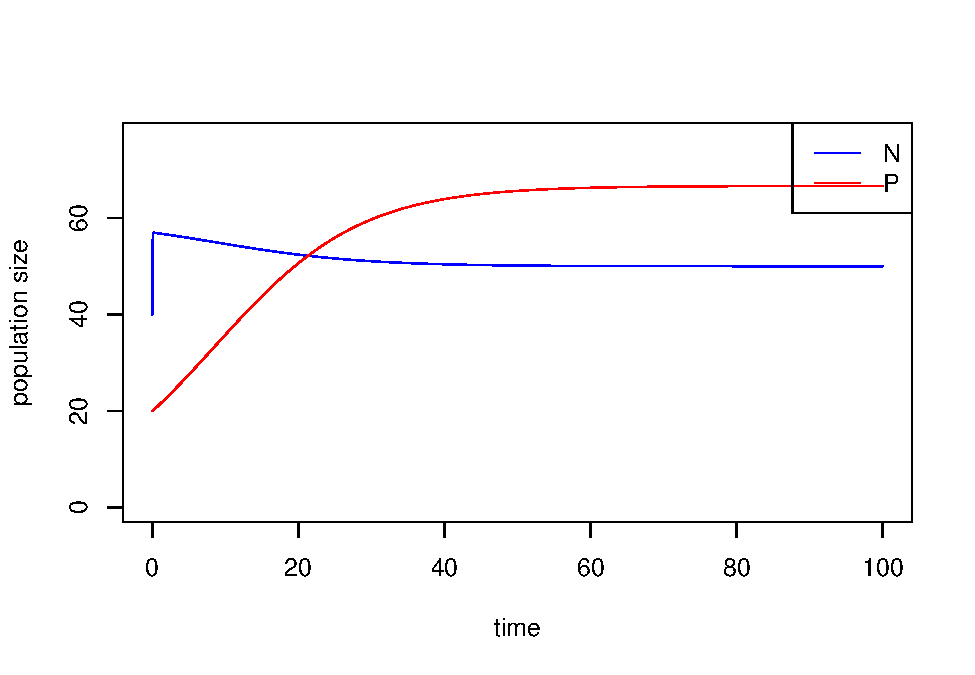
\includegraphics{bookdown-demo_files/figure-latex/unnamed-chunk-31-1.pdf}

\hypertarget{week-7---age-structure-population-model}{%
\chapter*{Week 7 - Age-structure population model}\label{week-7---age-structure-population-model}}
\addcontentsline{toc}{chapter}{Week 7 - Age-structure population model}

In this lab section, we will analyze a Leslie matrix using \texttt{for} loops and matrix algebra, compare the results with those obtained via eigen-analysis, and visualize the population dynamics and age distribution.

\textbf{Part 1 - Visualizing stable age distribution}

For any diagonalizable n-by-n matrix \(M\) with only one dominant eigenvalue, and for any n-by-1 vector \(v\), \(M^tv\) will shift to the same direction with the eigenvector of \(M\) corresponding to the dominant eigenvalue when \(t\) is large. Here, we visualize this fact numerically.

\begin{Shaded}
\begin{Highlighting}[]
\FunctionTok{library}\NormalTok{(ggplot2)}
\NormalTok{Time }\OtherTok{=} \DecValTok{6}
\NormalTok{A }\OtherTok{=} \FunctionTok{matrix}\NormalTok{(}\FunctionTok{c}\NormalTok{(}\DecValTok{1}\NormalTok{, }\DecValTok{1}\NormalTok{, }\FloatTok{0.5}\NormalTok{, }\DecValTok{0}\NormalTok{), }\DecValTok{2}\NormalTok{, }\DecValTok{2}\NormalTok{, }\AttributeTok{byrow=}\NormalTok{T)}
\NormalTok{N }\OtherTok{=} \FunctionTok{matrix}\NormalTok{(}\DecValTok{0}\NormalTok{, Time, }\DecValTok{2}\NormalTok{)}
\NormalTok{N[}\DecValTok{1}\NormalTok{, ] }\OtherTok{=} \FunctionTok{c}\NormalTok{(}\DecValTok{1}\NormalTok{, }\DecValTok{1}\NormalTok{)}
\ControlFlowTok{for}\NormalTok{(i }\ControlFlowTok{in} \DecValTok{2}\SpecialCharTok{:}\NormalTok{Time)\{}
\NormalTok{  N[i, ] }\OtherTok{=}\NormalTok{ A }\SpecialCharTok{\%*\%}\NormalTok{ N[i}\DecValTok{{-}1}\NormalTok{, ]}
\NormalTok{\}}
\NormalTok{Data }\OtherTok{=} \FunctionTok{as.data.frame}\NormalTok{(N)}
\NormalTok{Data}\SpecialCharTok{$}\NormalTok{Time }\OtherTok{=} \FunctionTok{rep}\NormalTok{(}\DecValTok{1}\SpecialCharTok{:}\NormalTok{Time)}
\NormalTok{Data}\SpecialCharTok{$}\NormalTok{V1.start }\OtherTok{=} \DecValTok{0}
\NormalTok{Data}\SpecialCharTok{$}\NormalTok{V2.start }\OtherTok{=} \DecValTok{0}

\FunctionTok{ggplot}\NormalTok{(Data, }\FunctionTok{aes}\NormalTok{(}\AttributeTok{x=}\NormalTok{V1, }\AttributeTok{y=}\NormalTok{V2, }\AttributeTok{col=}\FunctionTok{as.factor}\NormalTok{(Time))) }\SpecialCharTok{+} 
  \FunctionTok{geom\_point}\NormalTok{() }\SpecialCharTok{+} 
  \FunctionTok{geom\_segment}\NormalTok{(}\FunctionTok{aes}\NormalTok{(}\AttributeTok{x=}\NormalTok{V1.start, }\AttributeTok{y=}\NormalTok{V2.start, }\AttributeTok{xend=}\NormalTok{V1, }\AttributeTok{yend=}\NormalTok{V2), }
               \AttributeTok{arrow=}\FunctionTok{arrow}\NormalTok{(}\AttributeTok{type=}\StringTok{"closed"}\NormalTok{, }\AttributeTok{length=}\FunctionTok{unit}\NormalTok{(}\FloatTok{0.4}\NormalTok{,}\StringTok{"cm"}\NormalTok{))) }\SpecialCharTok{+} 
  \FunctionTok{geom\_text}\NormalTok{(}\FunctionTok{aes}\NormalTok{(}\AttributeTok{x=}\NormalTok{V1}\FloatTok{+0.1}\NormalTok{, }\AttributeTok{y=}\NormalTok{V2}\FloatTok{+0.1}\NormalTok{, }\AttributeTok{label=}\NormalTok{Time)) }\SpecialCharTok{+} 
  \FunctionTok{scale\_color\_brewer}\NormalTok{(}\StringTok{"Time"}\NormalTok{, }\AttributeTok{type=}\StringTok{"qual"}\NormalTok{, }\AttributeTok{palette=}\DecValTok{2}\NormalTok{) }\SpecialCharTok{+} 
  \FunctionTok{labs}\NormalTok{(}\AttributeTok{x=}\StringTok{"Age 1"}\NormalTok{, }\AttributeTok{y=}\StringTok{"Age 2"}\NormalTok{) }\SpecialCharTok{+}  
  \FunctionTok{theme\_classic}\NormalTok{()}
\end{Highlighting}
\end{Shaded}

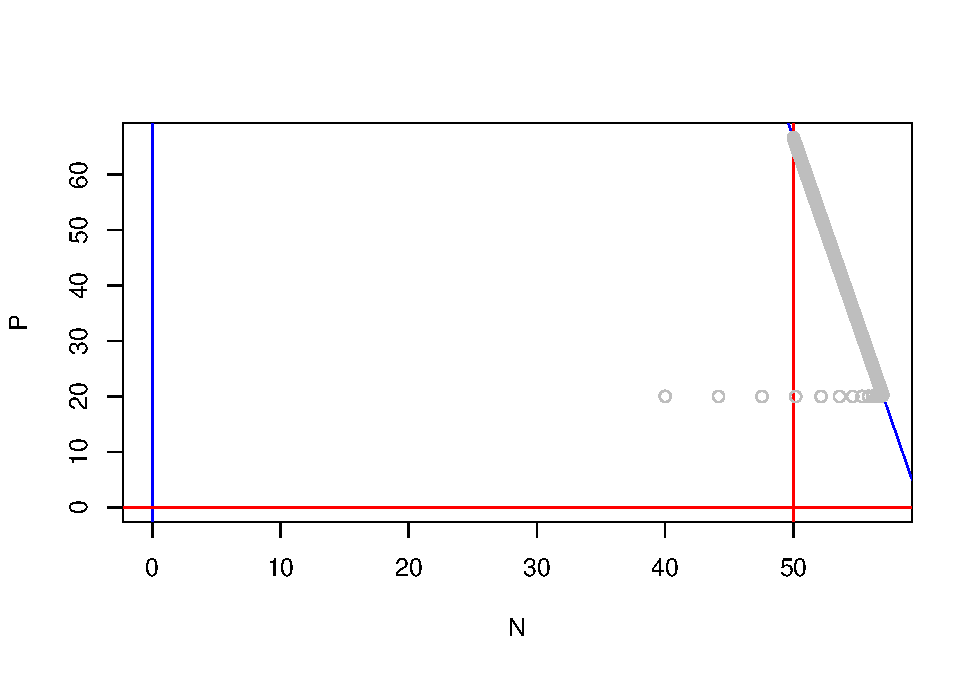
\includegraphics{bookdown-demo_files/figure-latex/unnamed-chunk-32-1.pdf}

\textbf{Part 2 - Analyzing Leslie matrix}

Consider an age-strutured population model
\[
n_{t} = L^tn_0
\]
where \(L\) is a Leslie matrix and \(n_t = (n_{1,t}, n_{2,t}, n_{3,t})\) is the population sizes with three different ages in time \(t\).

\begin{Shaded}
\begin{Highlighting}[]
\DocumentationTok{\#\#\# Leslie matrix and initial age classes}
\NormalTok{leslie }\OtherTok{\textless{}{-}} \FunctionTok{matrix}\NormalTok{(}\AttributeTok{data =} \FunctionTok{c}\NormalTok{(}\DecValTok{0}\NormalTok{, }\DecValTok{1}\NormalTok{, }\DecValTok{5}\NormalTok{,}
                          \FloatTok{0.5}\NormalTok{, }\DecValTok{0}\NormalTok{, }\DecValTok{0}\NormalTok{,}
                          \DecValTok{0}\NormalTok{, }\FloatTok{0.3}\NormalTok{, }\DecValTok{0}\NormalTok{),}
                      \AttributeTok{nrow =} \DecValTok{3}\NormalTok{,}
                      \AttributeTok{ncol =} \DecValTok{3}\NormalTok{,}
                      \AttributeTok{byrow =}\NormalTok{ T)}

\NormalTok{N0 }\OtherTok{\textless{}{-}} \FunctionTok{c}\NormalTok{(}\DecValTok{10}\NormalTok{, }\DecValTok{0}\NormalTok{, }\DecValTok{0}\NormalTok{)}

\DocumentationTok{\#\#\# for loop and matrix algebra}
\NormalTok{time }\OtherTok{\textless{}{-}} \DecValTok{50}
\NormalTok{pop\_size }\OtherTok{\textless{}{-}} \FunctionTok{data.frame}\NormalTok{(}\AttributeTok{Age1 =} \FunctionTok{rep}\NormalTok{(}\DecValTok{0}\NormalTok{, time),}
                       \AttributeTok{Age2 =} \FunctionTok{rep}\NormalTok{(}\DecValTok{0}\NormalTok{, time),}
                       \AttributeTok{Age3 =} \FunctionTok{rep}\NormalTok{(}\DecValTok{0}\NormalTok{, time))}
\NormalTok{pop\_size[}\DecValTok{1}\NormalTok{, ] }\OtherTok{\textless{}{-}}\NormalTok{ N0}

\ControlFlowTok{for}\NormalTok{ (i }\ControlFlowTok{in} \DecValTok{2}\SpecialCharTok{:}\NormalTok{time) \{}
  \CommentTok{\# Matrix multiplication}
\NormalTok{  pop\_size[i, ] }\OtherTok{\textless{}{-}}\NormalTok{ leslie }\SpecialCharTok{\%*\%} \FunctionTok{t}\NormalTok{(pop\_size[i}\DecValTok{{-}1}\NormalTok{, ])}
\NormalTok{\}}

\CommentTok{\# Total abundance}
\NormalTok{pop\_size}\SpecialCharTok{$}\NormalTok{N }\OtherTok{\textless{}{-}} \FunctionTok{rowSums}\NormalTok{(pop\_size)}

\FunctionTok{head}\NormalTok{(pop\_size)}
\end{Highlighting}
\end{Shaded}

\begin{verbatim}
##   Age1 Age2  Age3      N
## 1 10.0 0.00 0.000 10.000
## 2  0.0 5.00 0.000  5.000
## 3  5.0 0.00 1.500  6.500
## 4  7.5 2.50 0.000 10.000
## 5  2.5 3.75 0.750  7.000
## 6  7.5 1.25 1.125  9.875
\end{verbatim}

\begin{Shaded}
\begin{Highlighting}[]
\FunctionTok{plot}\NormalTok{(}\FunctionTok{c}\NormalTok{(}\DecValTok{1}\NormalTok{,time), }\FunctionTok{c}\NormalTok{(}\DecValTok{0}\NormalTok{,}\DecValTok{265}\NormalTok{), }\AttributeTok{type =} \StringTok{"n"}\NormalTok{, }\AttributeTok{xlab =} \StringTok{"time"}\NormalTok{, }\AttributeTok{ylab =} \StringTok{"pop\_size"}\NormalTok{)}
\FunctionTok{lines}\NormalTok{(}\DecValTok{1}\SpecialCharTok{:}\NormalTok{time , pop\_size}\SpecialCharTok{$}\NormalTok{Age1, }\AttributeTok{col =} \StringTok{"red"}\NormalTok{)}
\FunctionTok{lines}\NormalTok{(}\DecValTok{1}\SpecialCharTok{:}\NormalTok{time , pop\_size}\SpecialCharTok{$}\NormalTok{Age2, }\AttributeTok{col =} \StringTok{"blue"}\NormalTok{)}
\FunctionTok{lines}\NormalTok{(}\DecValTok{1}\SpecialCharTok{:}\NormalTok{time , pop\_size}\SpecialCharTok{$}\NormalTok{Age3, }\AttributeTok{col =} \StringTok{"green"}\NormalTok{)}
\FunctionTok{legend}\NormalTok{(}\StringTok{"topleft"}\NormalTok{,}
       \AttributeTok{legend =} \FunctionTok{c}\NormalTok{(}\StringTok{"Age1"}\NormalTok{, }\StringTok{"Age2"}\NormalTok{, }\StringTok{"Age3"}\NormalTok{),}
       \AttributeTok{col =} \FunctionTok{c}\NormalTok{(}\StringTok{"red"}\NormalTok{, }\StringTok{"blue"}\NormalTok{, }\StringTok{"green"}\NormalTok{),}
       \AttributeTok{lty =} \DecValTok{1}\NormalTok{)}
\end{Highlighting}
\end{Shaded}

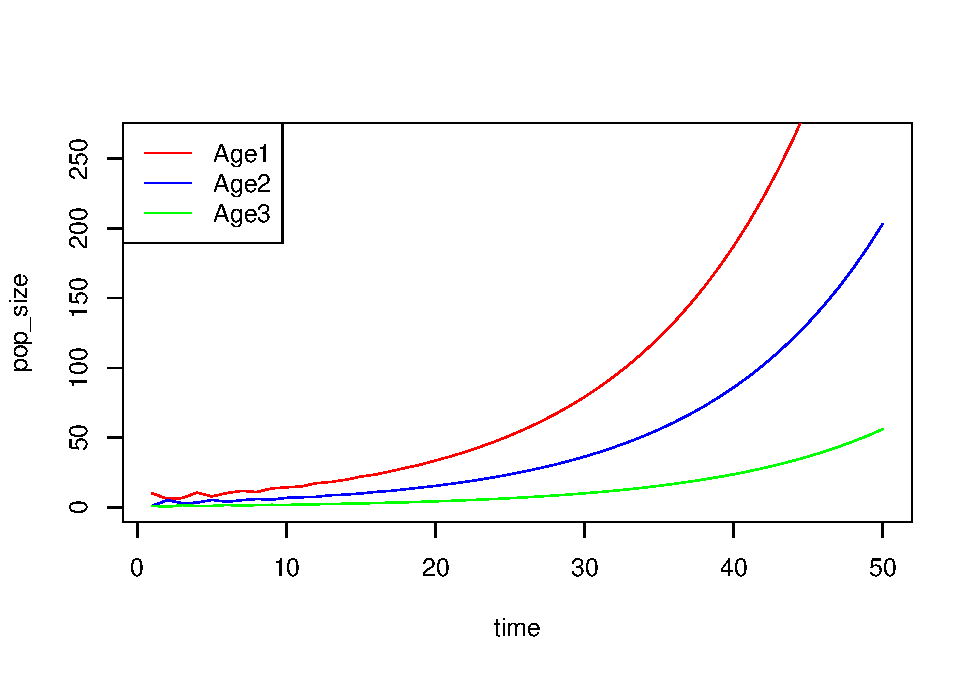
\includegraphics{bookdown-demo_files/figure-latex/unnamed-chunk-33-1.pdf}

Plot in log-scale:

\begin{Shaded}
\begin{Highlighting}[]
\FunctionTok{matplot}\NormalTok{(}\AttributeTok{x =} \DecValTok{1}\SpecialCharTok{:}\NormalTok{time, }\AttributeTok{y =} \FunctionTok{log}\NormalTok{(pop\_size[, }\DecValTok{1}\SpecialCharTok{:}\DecValTok{4}\NormalTok{]), }\AttributeTok{type =} \StringTok{"l"}\NormalTok{, }\AttributeTok{lty =} \DecValTok{1}\NormalTok{,}
        \AttributeTok{col =} \FunctionTok{c}\NormalTok{(}\StringTok{"red"}\NormalTok{, }\StringTok{"green"}\NormalTok{, }\StringTok{"blue"}\NormalTok{, }\StringTok{"black"}\NormalTok{),}
        \AttributeTok{xlab =} \StringTok{"Time"}\NormalTok{, }\AttributeTok{ylab =} \StringTok{"log(population size)"}\NormalTok{)}
\FunctionTok{legend}\NormalTok{(}\StringTok{"bottomright"}\NormalTok{, }\FunctionTok{c}\NormalTok{(}\StringTok{"Age 1"}\NormalTok{, }\StringTok{"Age 2"}\NormalTok{, }\StringTok{"Age 3"}\NormalTok{, }\StringTok{"Total"}\NormalTok{), }\AttributeTok{bty =} \StringTok{"n"}\NormalTok{,}
       \AttributeTok{lty =} \DecValTok{1}\NormalTok{ , }\AttributeTok{col =} \FunctionTok{c}\NormalTok{(}\StringTok{"red"}\NormalTok{, }\StringTok{"green"}\NormalTok{, }\StringTok{"blue"}\NormalTok{, }\StringTok{"black"}\NormalTok{))}
\end{Highlighting}
\end{Shaded}

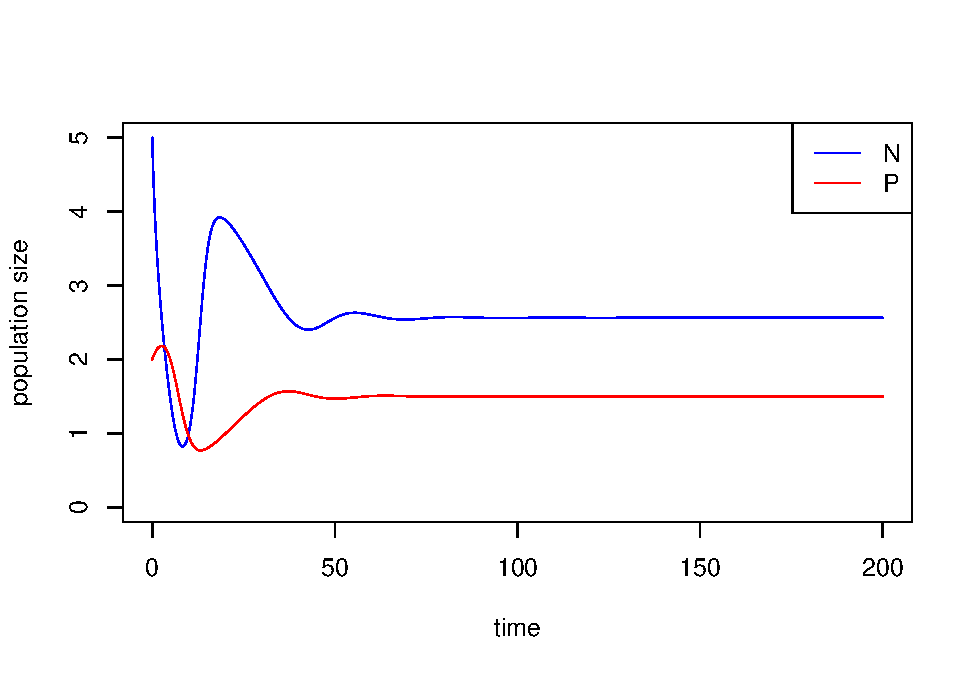
\includegraphics{bookdown-demo_files/figure-latex/unnamed-chunk-34-1.pdf}

By the derivation in the class, the asymptotic population sizes can be approximated by
\[
n_t \approx c\cdot \lambda_1^t\cdot u_1
\]
where \(c\) is a constant, \(\lambda_1\) is the dominant eigenvalue and \(u_1\) is the corresponding eigenvector. Hence, with the long-term dynamics, the population grows at a rate \(\lambda_1\) and with the age distribution \(u_1\). Here, we check this fact numerically.

\begin{Shaded}
\begin{Highlighting}[]
\DocumentationTok{\#\#\# Asymptotic growth rate and stable age distribution}

\NormalTok{asymptotic\_growth }\OtherTok{\textless{}{-}}\NormalTok{ pop\_size}\SpecialCharTok{$}\NormalTok{N[time]}\SpecialCharTok{/}\NormalTok{pop\_size}\SpecialCharTok{$}\NormalTok{N[time}\DecValTok{{-}1}\NormalTok{]}
\NormalTok{asymptotic\_growth}
\end{Highlighting}
\end{Shaded}

\begin{verbatim}
## [1] 1.089992
\end{verbatim}

\begin{Shaded}
\begin{Highlighting}[]
\NormalTok{age\_distribution }\OtherTok{\textless{}{-}}\NormalTok{ pop\_size[time, }\DecValTok{1}\SpecialCharTok{:}\DecValTok{3}\NormalTok{]}\SpecialCharTok{/}\FunctionTok{sum}\NormalTok{(pop\_size[time, }\DecValTok{1}\SpecialCharTok{:}\DecValTok{3}\NormalTok{])}
\NormalTok{age\_distribution}
\end{Highlighting}
\end{Shaded}

\begin{verbatim}
##         Age1      Age2       Age3
## 50 0.6309262 0.2894167 0.07965713
\end{verbatim}

\begin{Shaded}
\begin{Highlighting}[]
\DocumentationTok{\#\#\# Eigen{-}analysis of the Leslie matrix}
\NormalTok{EIGEN }\OtherTok{\textless{}{-}} \FunctionTok{eigen}\NormalTok{(leslie)}
\NormalTok{EIGEN}
\end{Highlighting}
\end{Shaded}

\begin{verbatim}
## eigen() decomposition
## $values
## [1]  1.0899905+0.0000000i -0.5449953+0.6253475i -0.5449953-0.6253475i
## 
## $vectors
##              [,1]                   [,2]                   [,3]
## [1,] 0.9030054+0i -0.84189720+0.0000000i -0.84189720+0.0000000i
## [2,] 0.4142263+0i  0.33341356+0.3825709i  0.33341356-0.3825709i
## [3,] 0.1140082+0i  0.02508328-0.1818099i  0.02508328+0.1818099i
\end{verbatim}

\begin{Shaded}
\begin{Highlighting}[]
\FunctionTok{abs}\NormalTok{(EIGEN}\SpecialCharTok{$}\NormalTok{values[}\DecValTok{1}\NormalTok{]) }\CommentTok{\# dominant eigenvalue}
\end{Highlighting}
\end{Shaded}

\begin{verbatim}
## [1] 1.089991
\end{verbatim}

\begin{Shaded}
\begin{Highlighting}[]
\FunctionTok{as.numeric}\NormalTok{(EIGEN}\SpecialCharTok{$}\NormalTok{vectors[, }\DecValTok{1}\NormalTok{] }\SpecialCharTok{/} \FunctionTok{sum}\NormalTok{(EIGEN}\SpecialCharTok{$}\NormalTok{vectors[, }\DecValTok{1}\NormalTok{])) }\CommentTok{\# corresponding eigenvector}
\end{Highlighting}
\end{Shaded}

\begin{verbatim}
## [1] 0.63092527 0.28941777 0.07965696
\end{verbatim}

The asymptotic growth rate and stable age distribution obtained from for loops and eigen-analysis are similar.

\textbf{Part 3 - In-class exercise: Analyzing population matrix of common teasel}

\href{https://en.wikipedia.org/wiki/Dipsacus_fullonum}{Common teasel (\emph{Dipsacus sylvestris})} is a herbaceous plant commonly found in abandoned fields and meadows in North America. It has a complex life cycle consisting of various stages. The seeds may lie dormant for one or two years. Seeds that germinate form small rosettes, which will gradually transit into medium and eventually large rosettes. These rosettes (all three sizes) may remain in the same stage for years before entering the next stage. After undergoing vernalization, large (and a few medium) rosettes will form stalks and flower in the upcoming summer, set seeds once, and die. Occasionally, the flowering plants will produce seeds that directly germinate into small/medium/large rosettes without entering dormancy.

Here is a transition diagram for the teasel. Please convert this diagram into a stage-based transition matrix (Lefkovitch matrix) and derive the asymptotic growth rate \(\lambda\) in R.

\begin{Shaded}
\begin{Highlighting}[]
\DocumentationTok{\#\#\# Leslie matrix for Teasel}
\NormalTok{Teasel }\OtherTok{\textless{}{-}} \FunctionTok{matrix}\NormalTok{(}\AttributeTok{data =} \FunctionTok{c}\NormalTok{(}\DecValTok{0}\NormalTok{,      }\DecValTok{0}\NormalTok{,      }\DecValTok{0}\NormalTok{,      }\DecValTok{0}\NormalTok{,      }\DecValTok{0}\NormalTok{,      }\FloatTok{322.38}\NormalTok{,}
                          \FloatTok{0.966}\NormalTok{,  }\DecValTok{0}\NormalTok{,      }\DecValTok{0}\NormalTok{,      }\DecValTok{0}\NormalTok{,      }\DecValTok{0}\NormalTok{,      }\DecValTok{0}\NormalTok{,}
                          \FloatTok{0.013}\NormalTok{,  }\FloatTok{0.010}\NormalTok{,  }\FloatTok{0.125}\NormalTok{,  }\DecValTok{0}\NormalTok{,      }\DecValTok{0}\NormalTok{,      }\FloatTok{3.448}\NormalTok{,}
                          \FloatTok{0.007}\NormalTok{,  }\DecValTok{0}\NormalTok{,      }\FloatTok{0.125}\NormalTok{,  }\FloatTok{0.238}\NormalTok{,  }\DecValTok{0}\NormalTok{,      }\FloatTok{30.17}\NormalTok{,}
                          \FloatTok{0.008}\NormalTok{,  }\DecValTok{0}\NormalTok{,      }\DecValTok{0}\NormalTok{,      }\FloatTok{0.245}\NormalTok{,  }\FloatTok{0.167}\NormalTok{,  }\FloatTok{0.862}\NormalTok{,}
                          \DecValTok{0}\NormalTok{,      }\DecValTok{0}\NormalTok{,      }\DecValTok{0}\NormalTok{,      }\FloatTok{0.023}\NormalTok{,  }\FloatTok{0.75}\NormalTok{,   }\DecValTok{0}\NormalTok{),}
                 \AttributeTok{nrow =} \DecValTok{6}\NormalTok{,}
                 \AttributeTok{ncol =} \DecValTok{6}\NormalTok{,}
                 \AttributeTok{byrow =}\NormalTok{ T)}
\DocumentationTok{\#\#\# Use eigen() function}
\NormalTok{EIGEN }\OtherTok{\textless{}{-}} \FunctionTok{eigen}\NormalTok{(Teasel)}
\DocumentationTok{\#\#\# Dominant eigenvalue}
\FunctionTok{abs}\NormalTok{(EIGEN}\SpecialCharTok{$}\NormalTok{values[}\DecValTok{1}\NormalTok{])}
\end{Highlighting}
\end{Shaded}

\begin{verbatim}
## [1] 2.32188
\end{verbatim}

\begin{Shaded}
\begin{Highlighting}[]
\DocumentationTok{\#\#\# corresponding eigenvector}
\FunctionTok{round}\NormalTok{(}\FunctionTok{as.numeric}\NormalTok{(EIGEN}\SpecialCharTok{$}\NormalTok{vectors[, }\DecValTok{1}\NormalTok{] }\SpecialCharTok{/} \FunctionTok{sum}\NormalTok{(EIGEN}\SpecialCharTok{$}\NormalTok{vectors[, }\DecValTok{1}\NormalTok{])), }\DecValTok{3}\NormalTok{)}
\end{Highlighting}
\end{Shaded}

\begin{verbatim}
## [1] 0.637 0.265 0.012 0.069 0.012 0.005
\end{verbatim}

\textbf{Part 4 - COM(P)ADRE: A global database of population matrices}

\href{https://compadre-db.org/ExploreDatabase}{COM(P)ADRE} is an online repository containing matrix population models on hundreds of plants, animals, algae, fungi, bacteria, and viruses around the world, as well as their associated metadata. Take a look at the website: You will be exploring the population dynamics of a species (of your choice) in your assignment!

\hypertarget{week-8---lotka-volterra-competition-model---population-dynamics}{%
\chapter*{Week 8 - Lotka-Volterra competition model - Population dynamics}\label{week-8---lotka-volterra-competition-model---population-dynamics}}
\addcontentsline{toc}{chapter}{Week 8 - Lotka-Volterra competition model - Population dynamics}

In this lab, we are going to analyze the two-species Lotka-Volterra competition model numerically and visualize the population dynamics under different parameter settings.

\textbf{Part 1 - Visualize the Population Dynamics with Time Series}

\begin{Shaded}
\begin{Highlighting}[]
\FunctionTok{library}\NormalTok{(ggplot2)}
\FunctionTok{library}\NormalTok{(tidyverse)}
\FunctionTok{library}\NormalTok{(deSolve)}

\NormalTok{LV\_model }\OtherTok{\textless{}{-}} \ControlFlowTok{function}\NormalTok{(}\AttributeTok{r1 =} \FloatTok{1.4}\NormalTok{, }\AttributeTok{r2 =} \FloatTok{1.2}\NormalTok{, }
                     \AttributeTok{a11 =} \DecValTok{1}\SpecialCharTok{/}\DecValTok{200}\NormalTok{, }\AttributeTok{a21 =} \DecValTok{1}\SpecialCharTok{/}\DecValTok{400}\NormalTok{, }\AttributeTok{a22 =} \DecValTok{1}\SpecialCharTok{/}\DecValTok{200}\NormalTok{, }\AttributeTok{a12 =} \DecValTok{1}\SpecialCharTok{/}\DecValTok{300}\NormalTok{, }
                     \AttributeTok{N1\_0 =} \DecValTok{10}\NormalTok{, }\AttributeTok{N2\_0 =} \DecValTok{10}\NormalTok{) \{}

  \DocumentationTok{\#\#\# Model specification}
\NormalTok{  LV }\OtherTok{\textless{}{-}} \ControlFlowTok{function}\NormalTok{(times, state, parms) \{}
    \FunctionTok{with}\NormalTok{(}\FunctionTok{as.list}\NormalTok{(}\FunctionTok{c}\NormalTok{(state, parms)), \{}
\NormalTok{      dN1\_dt }\OtherTok{=}\NormalTok{ N1 }\SpecialCharTok{*}\NormalTok{ (r1 }\SpecialCharTok{{-}}\NormalTok{ a11}\SpecialCharTok{*}\NormalTok{N1 }\SpecialCharTok{{-}}\NormalTok{ a12}\SpecialCharTok{*}\NormalTok{N2)}
\NormalTok{      dN2\_dt }\OtherTok{=}\NormalTok{ N2 }\SpecialCharTok{*}\NormalTok{ (r2 }\SpecialCharTok{{-}}\NormalTok{ a22}\SpecialCharTok{*}\NormalTok{N2 }\SpecialCharTok{{-}}\NormalTok{ a21}\SpecialCharTok{*}\NormalTok{N1)}
      \FunctionTok{return}\NormalTok{(}\FunctionTok{list}\NormalTok{(}\FunctionTok{c}\NormalTok{(dN1\_dt, dN2\_dt)))}
\NormalTok{    \})}
\NormalTok{  \}}

  \DocumentationTok{\#\#\# Model parameters}
\NormalTok{  times }\OtherTok{\textless{}{-}} \FunctionTok{seq}\NormalTok{(}\DecValTok{0}\NormalTok{, }\DecValTok{100}\NormalTok{, }\AttributeTok{by =} \FloatTok{0.1}\NormalTok{)}
\NormalTok{  state }\OtherTok{\textless{}{-}} \FunctionTok{c}\NormalTok{(}\AttributeTok{N1 =}\NormalTok{ N1\_0, }\AttributeTok{N2 =}\NormalTok{ N2\_0)}
\NormalTok{  parms }\OtherTok{\textless{}{-}} \FunctionTok{c}\NormalTok{(}\AttributeTok{r1 =}\NormalTok{ r1, }\AttributeTok{r2 =}\NormalTok{ r2, }\AttributeTok{a11 =}\NormalTok{ a11, }\AttributeTok{a21 =}\NormalTok{ a21, }\AttributeTok{a22 =}\NormalTok{ a22, }\AttributeTok{a12 =}\NormalTok{ a12)}

  \DocumentationTok{\#\#\# Model application}
\NormalTok{  pop\_size }\OtherTok{\textless{}{-}} \FunctionTok{ode}\NormalTok{(}\AttributeTok{func =}\NormalTok{ LV, }\AttributeTok{times =}\NormalTok{ times, }\AttributeTok{y =}\NormalTok{ state, }\AttributeTok{parms =}\NormalTok{ parms)}

  \DocumentationTok{\#\#\# Visualize the population dynamics}
  \FunctionTok{par}\NormalTok{(}\AttributeTok{mar =} \FunctionTok{c}\NormalTok{(}\FloatTok{5.1}\NormalTok{, }\FloatTok{4.1}\NormalTok{, }\FloatTok{4.1}\NormalTok{, }\FloatTok{8.1}\NormalTok{), }\AttributeTok{xpd =} \ConstantTok{TRUE}\NormalTok{)}
  \FunctionTok{plot}\NormalTok{(N1 }\SpecialCharTok{\textasciitilde{}}\NormalTok{ time, }\AttributeTok{data =}\NormalTok{ pop\_size,}
       \AttributeTok{col =} \StringTok{"lightblue"}\NormalTok{, }\AttributeTok{type =} \StringTok{"l"}\NormalTok{, }\AttributeTok{lwd =} \DecValTok{3}\NormalTok{,}
       \AttributeTok{las =} \DecValTok{1}\NormalTok{,}
       \AttributeTok{xlim =} \FunctionTok{c}\NormalTok{(}\DecValTok{0}\NormalTok{, }\FunctionTok{max}\NormalTok{(times)), }\AttributeTok{ylim =} \FunctionTok{c}\NormalTok{(}\DecValTok{0}\NormalTok{, }\FunctionTok{max}\NormalTok{(pop\_size[,}\SpecialCharTok{{-}}\DecValTok{1}\NormalTok{])),}
       \AttributeTok{xlab =} \StringTok{"Time"}\NormalTok{,}
       \AttributeTok{ylab =} \StringTok{"Population size"}\NormalTok{,}
       \AttributeTok{main =} \StringTok{"Lotka{-}Volterra competition"}\NormalTok{)}
  \FunctionTok{lines}\NormalTok{(N2 }\SpecialCharTok{\textasciitilde{}}\NormalTok{ time, }\AttributeTok{data =}\NormalTok{ pop\_size, }\AttributeTok{col =} \StringTok{"pink"}\NormalTok{, }\AttributeTok{lwd =} \DecValTok{3}\NormalTok{)}
  \FunctionTok{legend}\NormalTok{(}\StringTok{"topright"}\NormalTok{,}
       \FunctionTok{c}\NormalTok{(}\StringTok{"N1"}\NormalTok{, }\StringTok{"N2"}\NormalTok{),}
       \AttributeTok{lty =} \DecValTok{1}\NormalTok{, }\AttributeTok{lwd =} \DecValTok{3}\NormalTok{,}
       \AttributeTok{col =} \FunctionTok{c}\NormalTok{(}\StringTok{"lightblue"}\NormalTok{, }\StringTok{"pink"}\NormalTok{),}
       \AttributeTok{bty =} \StringTok{"n"}\NormalTok{,}
       \AttributeTok{inset =} \FunctionTok{c}\NormalTok{(}\SpecialCharTok{{-}}\FloatTok{0.2}\NormalTok{,}\DecValTok{0}\NormalTok{),}
       \AttributeTok{title =} \StringTok{"Species"}
\NormalTok{       )}
\NormalTok{\}}
\end{Highlighting}
\end{Shaded}

Plot the population dynamics under different parameter sets.

\begin{Shaded}
\begin{Highlighting}[]
  \DocumentationTok{\#\#\# Different parameter settings}
  \DocumentationTok{\#\# N1\_0 = 200 and N2\_0 = 5}
  \FunctionTok{LV\_model}\NormalTok{(}\AttributeTok{r1 =} \FloatTok{1.2}\NormalTok{, }\AttributeTok{r2 =} \FloatTok{1.2}\NormalTok{, }
           \AttributeTok{a11 =} \DecValTok{1}\SpecialCharTok{/}\DecValTok{200}\NormalTok{, }\AttributeTok{a21 =} \DecValTok{1}\SpecialCharTok{/}\DecValTok{100}\NormalTok{, }\AttributeTok{a22 =} \DecValTok{1}\SpecialCharTok{/}\DecValTok{100}\NormalTok{, }\AttributeTok{a12 =} \DecValTok{1}\SpecialCharTok{/}\DecValTok{200}\NormalTok{, }
           \AttributeTok{N1\_0 =} \DecValTok{200}\NormalTok{, }\AttributeTok{N2\_0 =} \DecValTok{5}\NormalTok{)  }\CommentTok{\# N1 wins}
\end{Highlighting}
\end{Shaded}

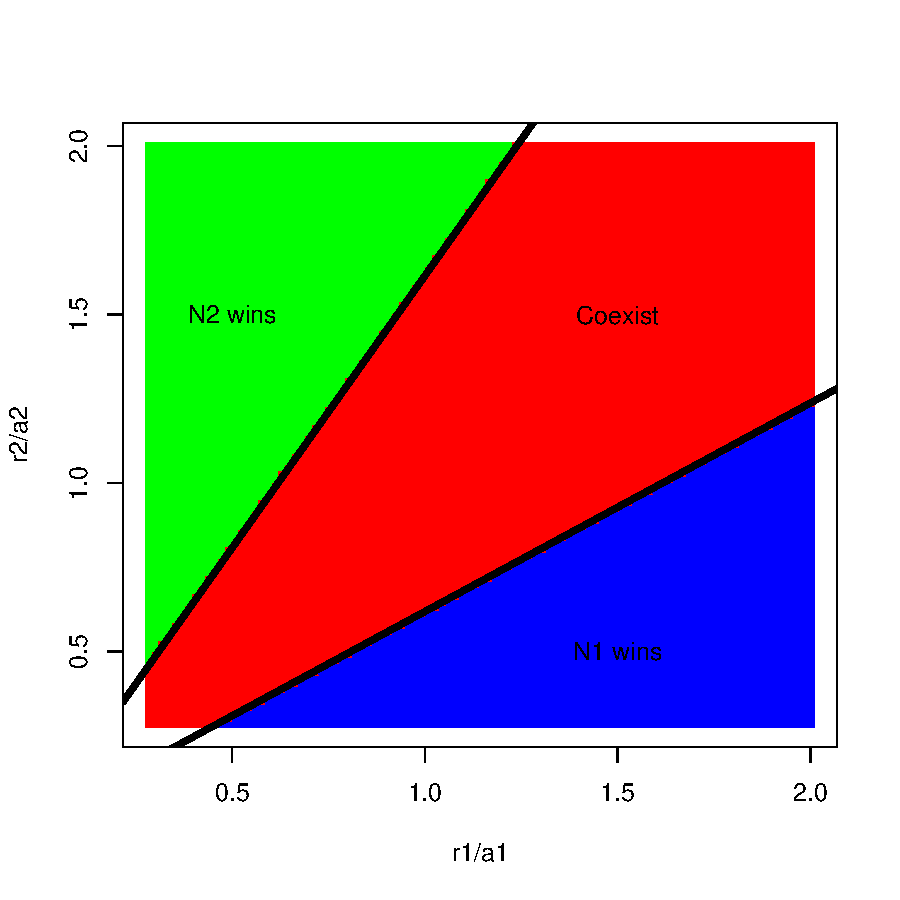
\includegraphics{bookdown-demo_files/figure-latex/unnamed-chunk-38-1.pdf}

\begin{Shaded}
\begin{Highlighting}[]
  \DocumentationTok{\#\# N1\_0 = 5 and N2\_0 = 200}
  \FunctionTok{LV\_model}\NormalTok{(}\AttributeTok{r1 =} \FloatTok{1.2}\NormalTok{, }\AttributeTok{r2 =} \FloatTok{1.2}\NormalTok{, }
           \AttributeTok{a11 =} \DecValTok{1}\SpecialCharTok{/}\DecValTok{200}\NormalTok{, }\AttributeTok{a21 =} \DecValTok{1}\SpecialCharTok{/}\DecValTok{100}\NormalTok{, }\AttributeTok{a22 =} \DecValTok{1}\SpecialCharTok{/}\DecValTok{100}\NormalTok{, }\AttributeTok{a12 =} \DecValTok{1}\SpecialCharTok{/}\DecValTok{200}\NormalTok{, }
           \AttributeTok{N1\_0 =} \DecValTok{10}\NormalTok{, }\AttributeTok{N2\_0 =} \DecValTok{200}\NormalTok{)  }\CommentTok{\# N1 wins}
\end{Highlighting}
\end{Shaded}

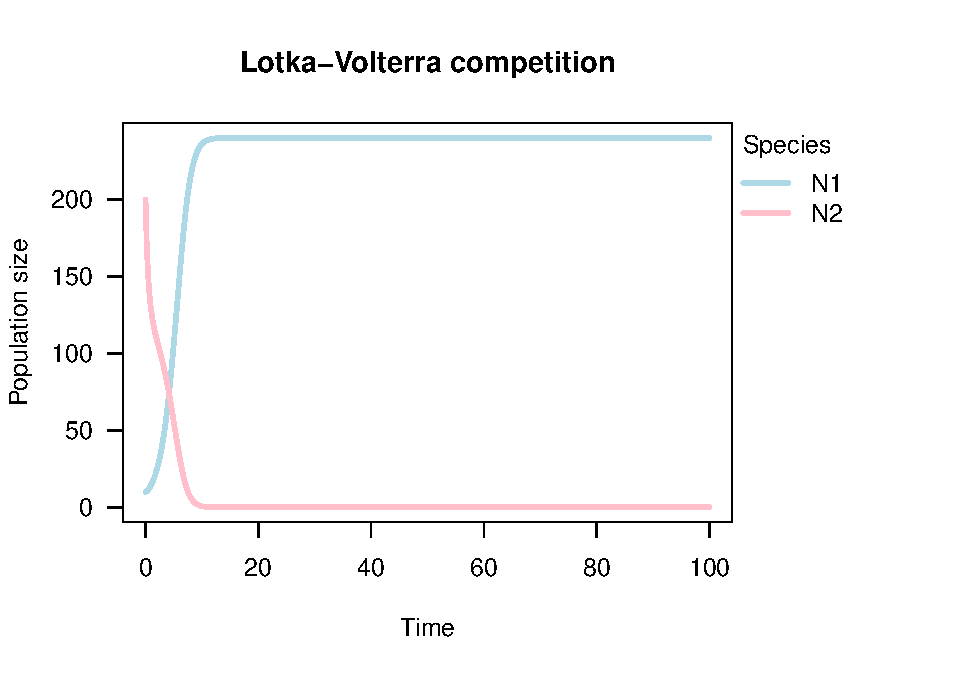
\includegraphics{bookdown-demo_files/figure-latex/unnamed-chunk-38-2.pdf}

\begin{Shaded}
\begin{Highlighting}[]
  \DocumentationTok{\#\# N1\_0 = 200 and N2\_0 = 5}
  \FunctionTok{LV\_model}\NormalTok{(}\AttributeTok{r1 =} \FloatTok{1.2}\NormalTok{, }\AttributeTok{r2 =} \FloatTok{1.2}\NormalTok{, }
           \AttributeTok{a11 =} \DecValTok{1}\SpecialCharTok{/}\DecValTok{100}\NormalTok{, }\AttributeTok{a21 =} \DecValTok{1}\SpecialCharTok{/}\DecValTok{200}\NormalTok{, }\AttributeTok{a22 =} \DecValTok{1}\SpecialCharTok{/}\DecValTok{200}\NormalTok{, }\AttributeTok{a12 =} \DecValTok{1}\SpecialCharTok{/}\DecValTok{100}\NormalTok{, }
           \AttributeTok{N1\_0 =} \DecValTok{200}\NormalTok{, }\AttributeTok{N2\_0 =} \DecValTok{5}\NormalTok{)  }\CommentTok{\# N2 wins}
\end{Highlighting}
\end{Shaded}

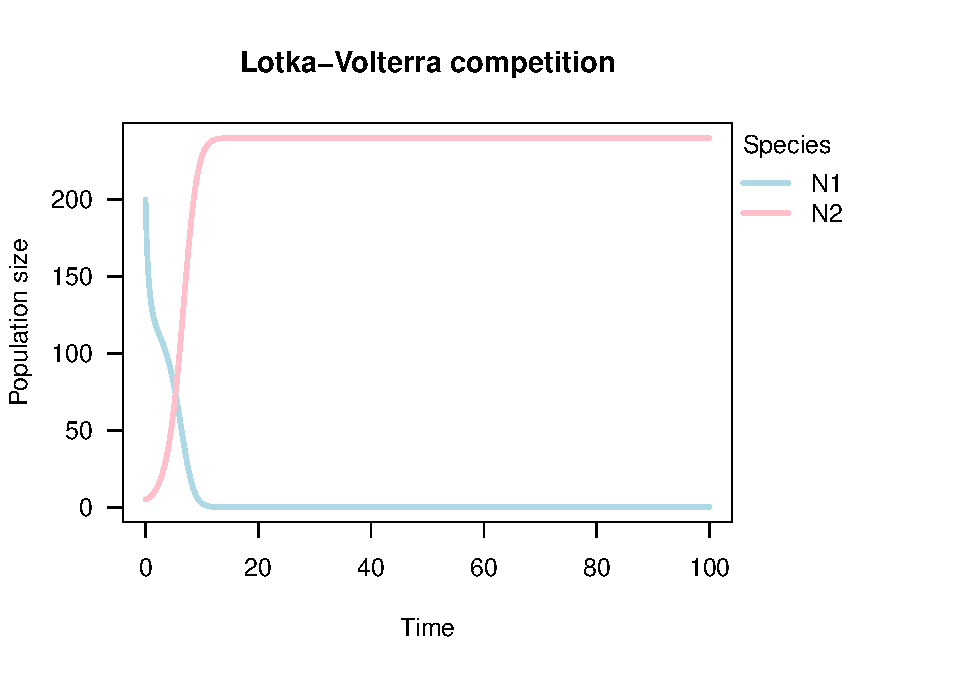
\includegraphics{bookdown-demo_files/figure-latex/unnamed-chunk-38-3.pdf}

\begin{Shaded}
\begin{Highlighting}[]
  \DocumentationTok{\#\# N1\_0 = 5 and N2\_0 = 200}
  \FunctionTok{LV\_model}\NormalTok{(}\AttributeTok{r1 =} \FloatTok{1.2}\NormalTok{, }\AttributeTok{r2 =} \FloatTok{1.2}\NormalTok{, }
           \AttributeTok{a11 =} \DecValTok{1}\SpecialCharTok{/}\DecValTok{100}\NormalTok{, }\AttributeTok{a21 =} \DecValTok{1}\SpecialCharTok{/}\DecValTok{200}\NormalTok{, }\AttributeTok{a22 =} \DecValTok{1}\SpecialCharTok{/}\DecValTok{200}\NormalTok{, }\AttributeTok{a12 =} \DecValTok{1}\SpecialCharTok{/}\DecValTok{100}\NormalTok{, }
           \AttributeTok{N1\_0 =} \DecValTok{5}\NormalTok{, }\AttributeTok{N2\_0 =} \DecValTok{200}\NormalTok{)  }\CommentTok{\# N2 wins}
\end{Highlighting}
\end{Shaded}

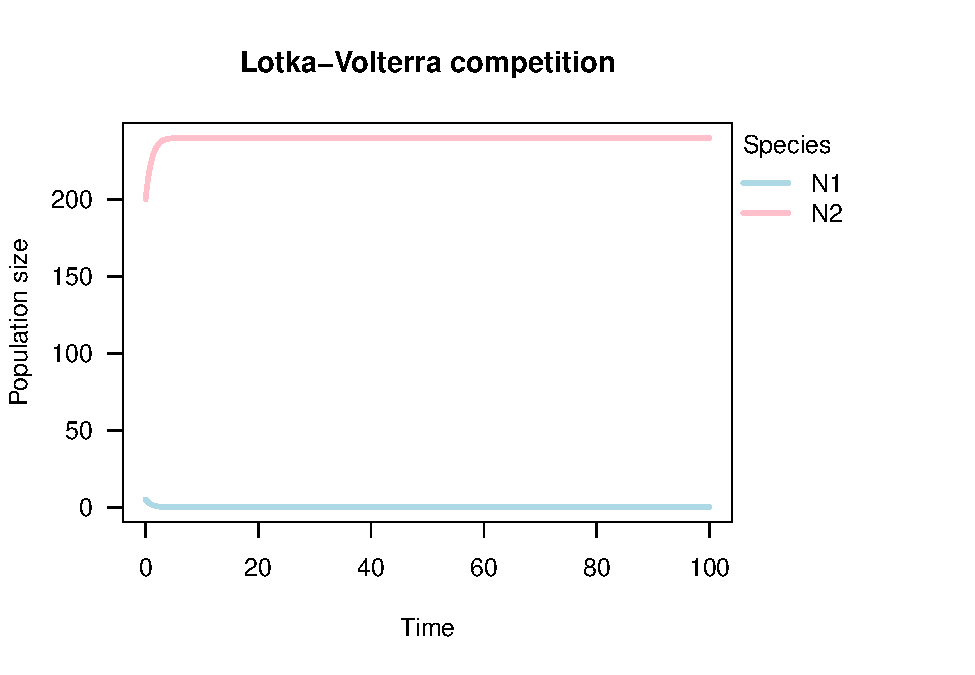
\includegraphics{bookdown-demo_files/figure-latex/unnamed-chunk-38-4.pdf}

\begin{Shaded}
\begin{Highlighting}[]
  \DocumentationTok{\#\# N1\_0 = 200 and N2\_0 = 5}
  \FunctionTok{LV\_model}\NormalTok{(}\AttributeTok{r1 =} \FloatTok{1.2}\NormalTok{, }\AttributeTok{r2 =} \FloatTok{1.2}\NormalTok{, }
           \AttributeTok{a11 =} \DecValTok{1}\SpecialCharTok{/}\DecValTok{100}\NormalTok{, }\AttributeTok{a21 =} \DecValTok{1}\SpecialCharTok{/}\DecValTok{200}\NormalTok{, }\AttributeTok{a22 =} \DecValTok{1}\SpecialCharTok{/}\DecValTok{100}\NormalTok{, }\AttributeTok{a12 =} \DecValTok{1}\SpecialCharTok{/}\DecValTok{300}\NormalTok{, }
           \AttributeTok{N1\_0 =} \DecValTok{200}\NormalTok{, }\AttributeTok{N2\_0 =} \DecValTok{5}\NormalTok{)  }\CommentTok{\# stable coexistence}
\end{Highlighting}
\end{Shaded}

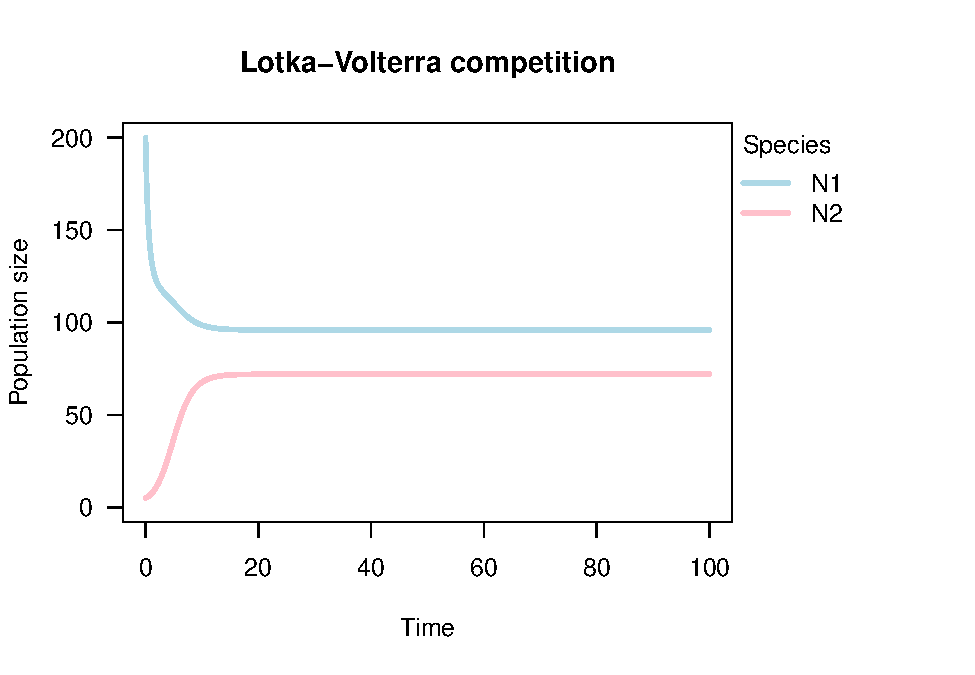
\includegraphics{bookdown-demo_files/figure-latex/unnamed-chunk-38-5.pdf}

\begin{Shaded}
\begin{Highlighting}[]
  \DocumentationTok{\#\# N1\_0 = 5 and N2\_0 = 200}
  \FunctionTok{LV\_model}\NormalTok{(}\AttributeTok{r1 =} \FloatTok{1.2}\NormalTok{, }\AttributeTok{r2 =} \FloatTok{1.2}\NormalTok{, }\AttributeTok{a11 =} \DecValTok{1}\SpecialCharTok{/}\DecValTok{100}\NormalTok{, }\AttributeTok{a21 =} \DecValTok{1}\SpecialCharTok{/}\DecValTok{200}\NormalTok{, }\AttributeTok{a22 =} \DecValTok{1}\SpecialCharTok{/}\DecValTok{100}\NormalTok{, }\AttributeTok{a12 =} \DecValTok{1}\SpecialCharTok{/}\DecValTok{300}\NormalTok{, }\AttributeTok{N1\_0 =} \DecValTok{5}\NormalTok{, }\AttributeTok{N2\_0 =} \DecValTok{200}\NormalTok{)  }\CommentTok{\# stable coexistence}
\end{Highlighting}
\end{Shaded}

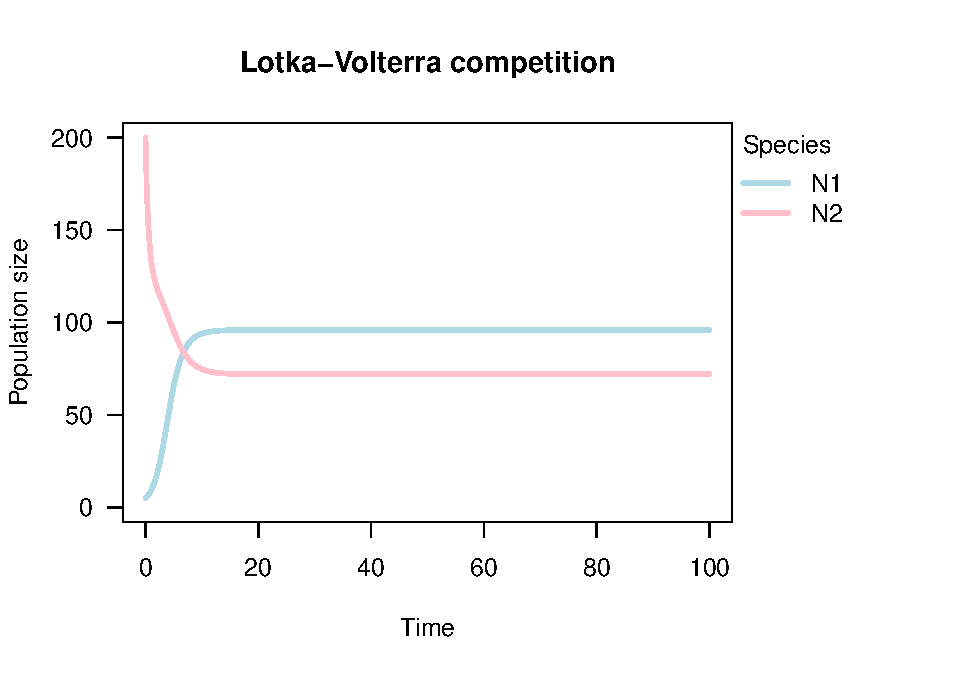
\includegraphics{bookdown-demo_files/figure-latex/unnamed-chunk-38-6.pdf}

\begin{Shaded}
\begin{Highlighting}[]
  \DocumentationTok{\#\# N1\_0 = 200 and N2\_0 = 150}
  \FunctionTok{LV\_model}\NormalTok{(}\AttributeTok{r1 =} \FloatTok{1.2}\NormalTok{, }\AttributeTok{r2 =} \FloatTok{1.2}\NormalTok{, }
           \AttributeTok{a11 =} \DecValTok{1}\SpecialCharTok{/}\DecValTok{200}\NormalTok{, }\AttributeTok{a21 =} \DecValTok{1}\SpecialCharTok{/}\DecValTok{100}\NormalTok{, }\AttributeTok{a22 =} \DecValTok{1}\SpecialCharTok{/}\DecValTok{200}\NormalTok{, }\AttributeTok{a12 =} \DecValTok{1}\SpecialCharTok{/}\DecValTok{100}\NormalTok{, }
           \AttributeTok{N1\_0 =} \DecValTok{200}\NormalTok{, }\AttributeTok{N2\_0 =} \DecValTok{150}\NormalTok{)  }\CommentTok{\# priority effect (N1 wins)}
\end{Highlighting}
\end{Shaded}

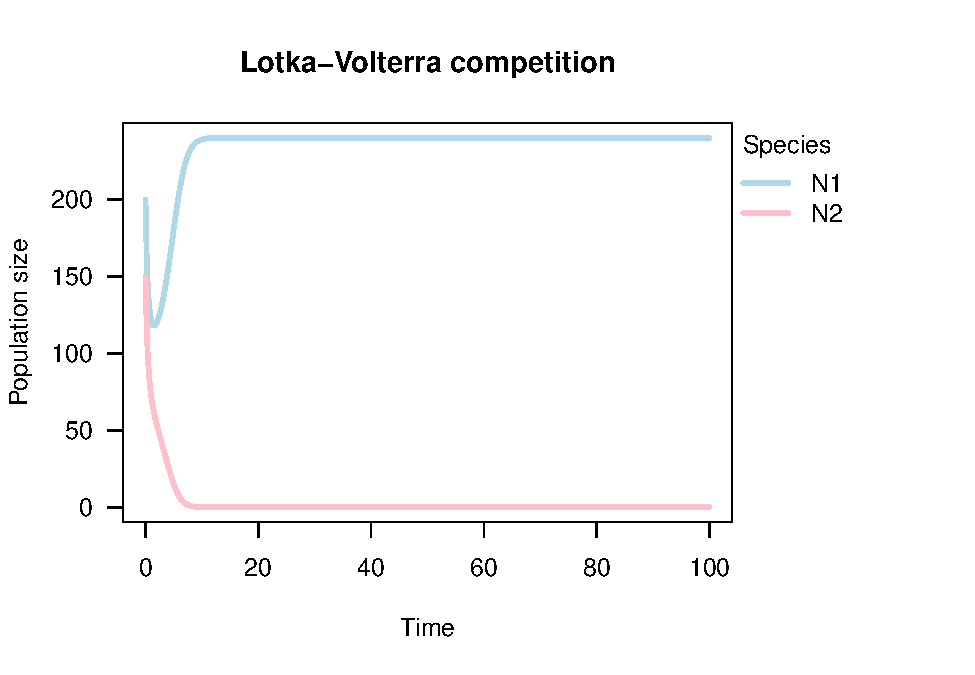
\includegraphics{bookdown-demo_files/figure-latex/unnamed-chunk-38-7.pdf}

\begin{Shaded}
\begin{Highlighting}[]
  \DocumentationTok{\#\# N1\_0 = 150 and N2\_0 = 200}
  \FunctionTok{LV\_model}\NormalTok{(}\AttributeTok{r1 =} \FloatTok{1.2}\NormalTok{, }\AttributeTok{r2 =} \FloatTok{1.2}\NormalTok{, }
           \AttributeTok{a11 =} \DecValTok{1}\SpecialCharTok{/}\DecValTok{200}\NormalTok{, }\AttributeTok{a21 =} \DecValTok{1}\SpecialCharTok{/}\DecValTok{100}\NormalTok{, }\AttributeTok{a22 =} \DecValTok{1}\SpecialCharTok{/}\DecValTok{200}\NormalTok{, }\AttributeTok{a12 =} \DecValTok{1}\SpecialCharTok{/}\DecValTok{100}\NormalTok{, }
           \AttributeTok{N1\_0 =} \DecValTok{150}\NormalTok{, }\AttributeTok{N2\_0 =} \DecValTok{200}\NormalTok{)  }\CommentTok{\# priority effect (N2 wins)}
\end{Highlighting}
\end{Shaded}

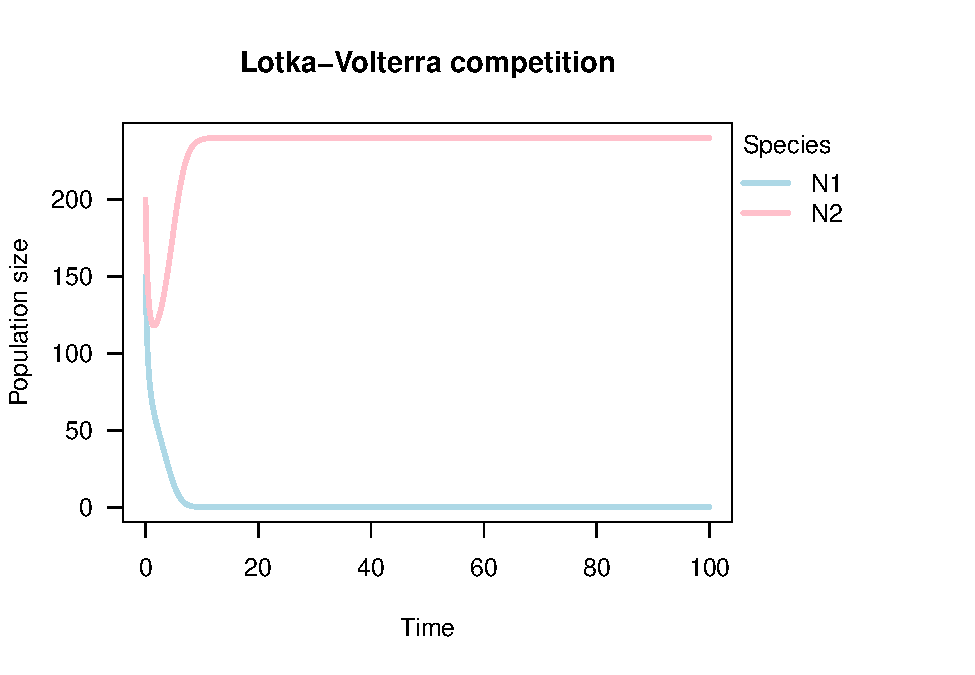
\includegraphics{bookdown-demo_files/figure-latex/unnamed-chunk-38-8.pdf}

\textbf{Part 2 - Visualize the Population Dynamics with State Space}

\begin{Shaded}
\begin{Highlighting}[]
\DocumentationTok{\#\#\#\# phase diagram}
\NormalTok{phase\_plane }\OtherTok{\textless{}{-}} \ControlFlowTok{function}\NormalTok{(r1, r2, a11, a21, a22, a12, title, t)\{}
    \DocumentationTok{\#\#\# Vectors}
\NormalTok{  LV }\OtherTok{\textless{}{-}} \ControlFlowTok{function}\NormalTok{(times, state, parms) \{}
    \FunctionTok{with}\NormalTok{(}\FunctionTok{as.list}\NormalTok{(}\FunctionTok{c}\NormalTok{(state, parms)), \{}
\NormalTok{      dN1\_dt }\OtherTok{=}\NormalTok{ N1 }\SpecialCharTok{*}\NormalTok{ (r1 }\SpecialCharTok{{-}}\NormalTok{ a11}\SpecialCharTok{*}\NormalTok{N1 }\SpecialCharTok{{-}}\NormalTok{ a12}\SpecialCharTok{*}\NormalTok{N2)}
\NormalTok{      dN2\_dt }\OtherTok{=}\NormalTok{ N2 }\SpecialCharTok{*}\NormalTok{ (r2 }\SpecialCharTok{{-}}\NormalTok{ a22}\SpecialCharTok{*}\NormalTok{N2 }\SpecialCharTok{{-}}\NormalTok{ a21}\SpecialCharTok{*}\NormalTok{N1)}
      \FunctionTok{return}\NormalTok{(}\FunctionTok{list}\NormalTok{(}\FunctionTok{c}\NormalTok{(dN1\_dt, dN2\_dt)))}
\NormalTok{    \})}
\NormalTok{  \}}

\NormalTok{  times }\OtherTok{\textless{}{-}} \FunctionTok{c}\NormalTok{(}\DecValTok{0}\NormalTok{, t)}
\NormalTok{  parms }\OtherTok{\textless{}{-}} \FunctionTok{c}\NormalTok{(}\AttributeTok{r1 =}\NormalTok{ r1, }\AttributeTok{r2 =}\NormalTok{ r2, }\AttributeTok{a11 =}\NormalTok{ a11, }\AttributeTok{a21 =}\NormalTok{ a21, }\AttributeTok{a22 =}\NormalTok{ a22, }\AttributeTok{a12 =}\NormalTok{ a12)}

\NormalTok{  x\_inter}\OtherTok{\textless{}{-}} \FunctionTok{max}\NormalTok{(}\FunctionTok{c}\NormalTok{(r1}\SpecialCharTok{/}\NormalTok{a11, r2}\SpecialCharTok{/}\NormalTok{a21))}
\NormalTok{  y\_inter }\OtherTok{\textless{}{-}} \FunctionTok{max}\NormalTok{(}\FunctionTok{c}\NormalTok{(r2}\SpecialCharTok{/}\NormalTok{a22, r1}\SpecialCharTok{/}\NormalTok{a12))}

  \CommentTok{\# create position of arrows}
\NormalTok{  vector\_grid }\OtherTok{\textless{}{-}} \FunctionTok{expand.grid}\NormalTok{(}\FunctionTok{seq}\NormalTok{(}\DecValTok{5}\NormalTok{, x\_inter, }\AttributeTok{length.out =} \DecValTok{10}\NormalTok{),}
                             \FunctionTok{seq}\NormalTok{(}\DecValTok{5}\NormalTok{, y\_inter, }\AttributeTok{length.out =} \DecValTok{10}\NormalTok{))}

\NormalTok{  vector\_data }\OtherTok{\textless{}{-}}\NormalTok{ vector\_grid }\SpecialCharTok{\%\textgreater{}\%}
    \FunctionTok{pmap}\NormalTok{(., }\ControlFlowTok{function}\NormalTok{(Var1, Var2)\{}
\NormalTok{      state }\OtherTok{\textless{}{-}} \FunctionTok{c}\NormalTok{(}\AttributeTok{N1 =}\NormalTok{ Var1, }\AttributeTok{N2 =}\NormalTok{ Var2)}
\NormalTok{      pop\_size }\OtherTok{\textless{}{-}} \FunctionTok{ode}\NormalTok{(}\AttributeTok{func =}\NormalTok{ LV, }\AttributeTok{times =}\NormalTok{ times, }\AttributeTok{y =}\NormalTok{ state, }\AttributeTok{parms =}\NormalTok{ parms)}
\NormalTok{      pop\_size[}\DecValTok{2}\NormalTok{, }\DecValTok{2}\SpecialCharTok{:}\DecValTok{3}\NormalTok{]}
\NormalTok{    \}) }\SpecialCharTok{\%\textgreater{}\%}
    \FunctionTok{bind\_rows}\NormalTok{() }\SpecialCharTok{\%\textgreater{}\%}
    \FunctionTok{rename}\NormalTok{(}\AttributeTok{xend =}\NormalTok{ N1, }\AttributeTok{yend =}\NormalTok{ N2) }\SpecialCharTok{\%\textgreater{}\%}
    \FunctionTok{bind\_cols}\NormalTok{(vector\_grid) }\SpecialCharTok{\%\textgreater{}\%}
    \FunctionTok{rename}\NormalTok{(}\AttributeTok{x =}\NormalTok{ Var1, }\AttributeTok{y =}\NormalTok{ Var2)}

    \DocumentationTok{\#\#\# Phase plane}
    \FunctionTok{ggplot}\NormalTok{() }\SpecialCharTok{+}
      \FunctionTok{geom\_abline}\NormalTok{(}\AttributeTok{slope =} \SpecialCharTok{{-}}\NormalTok{a11}\SpecialCharTok{/}\NormalTok{a12, }\AttributeTok{intercept =}\NormalTok{ r1}\SpecialCharTok{/}\NormalTok{a12, }
                  \AttributeTok{color =} \StringTok{"\#E41A1C"}\NormalTok{, }\AttributeTok{size =} \FloatTok{1.5}\NormalTok{) }\SpecialCharTok{+}
      \FunctionTok{geom\_abline}\NormalTok{(}\AttributeTok{slope =} \SpecialCharTok{{-}}\NormalTok{a21}\SpecialCharTok{/}\NormalTok{a22, }\AttributeTok{intercept =}\NormalTok{ r2}\SpecialCharTok{/}\NormalTok{a22, }
                  \AttributeTok{color =} \StringTok{"\#377EB8"}\NormalTok{, }\AttributeTok{size =} \FloatTok{1.5}\NormalTok{) }\SpecialCharTok{+}
      \FunctionTok{geom\_segment}\NormalTok{(}\AttributeTok{data =}\NormalTok{ vector\_data,}
                   \FunctionTok{aes}\NormalTok{(}\AttributeTok{x =}\NormalTok{ x, }\AttributeTok{y =}\NormalTok{ y, }\AttributeTok{xend =}\NormalTok{ xend, }\AttributeTok{yend =}\NormalTok{ yend),}
                   \AttributeTok{arrow =} \FunctionTok{arrow}\NormalTok{(}\AttributeTok{length =} \FunctionTok{unit}\NormalTok{(}\FloatTok{0.1}\NormalTok{, }\StringTok{"cm"}\NormalTok{))) }\SpecialCharTok{+}    
      \FunctionTok{scale\_x\_continuous}\NormalTok{(}\AttributeTok{name =} \StringTok{"N1"}\NormalTok{, }\AttributeTok{limits =} \FunctionTok{c}\NormalTok{(}\DecValTok{0}\NormalTok{, x\_inter), }\AttributeTok{expand =} \FunctionTok{c}\NormalTok{(}\DecValTok{0}\NormalTok{, }\DecValTok{0}\NormalTok{)) }\SpecialCharTok{+}
      \FunctionTok{scale\_y\_continuous}\NormalTok{(}\AttributeTok{name =} \StringTok{"N2"}\NormalTok{, }\AttributeTok{limits =} \FunctionTok{c}\NormalTok{(}\DecValTok{0}\NormalTok{, y\_inter), }\AttributeTok{expand =} \FunctionTok{c}\NormalTok{(}\DecValTok{0}\NormalTok{, }\DecValTok{0}\NormalTok{)) }\SpecialCharTok{+}
      \FunctionTok{theme\_bw}\NormalTok{(}\AttributeTok{base\_size =} \DecValTok{13}\NormalTok{) }\SpecialCharTok{+}
      \FunctionTok{theme}\NormalTok{(}\AttributeTok{panel.grid =} \FunctionTok{element\_blank}\NormalTok{(),}
            \AttributeTok{plot.title =} \FunctionTok{element\_text}\NormalTok{(}\AttributeTok{hjust =} \FloatTok{0.5}\NormalTok{),}
            \AttributeTok{aspect.ratio =} \DecValTok{1}\NormalTok{) }\SpecialCharTok{+}
      \FunctionTok{labs}\NormalTok{(}\AttributeTok{title =}\NormalTok{ title)}
\NormalTok{  \}}
\end{Highlighting}
\end{Shaded}

Plot the population dynamics under different parameter sets.

\begin{Shaded}
\begin{Highlighting}[]
  \FunctionTok{phase\_plane}\NormalTok{(}\AttributeTok{r1 =} \FloatTok{1.2}\NormalTok{, }\AttributeTok{r2 =} \FloatTok{1.2}\NormalTok{, }\AttributeTok{a11 =} \DecValTok{1}\SpecialCharTok{/}\DecValTok{100}\NormalTok{, }
              \AttributeTok{a21 =} \DecValTok{1}\SpecialCharTok{/}\DecValTok{200}\NormalTok{, }\AttributeTok{a22 =} \DecValTok{1}\SpecialCharTok{/}\DecValTok{100}\NormalTok{, }\AttributeTok{a12 =} \DecValTok{1}\SpecialCharTok{/}\DecValTok{200}\NormalTok{, }
              \AttributeTok{t =} \FloatTok{0.2}\NormalTok{, }\AttributeTok{title =} \StringTok{"Stable coexistence"}\NormalTok{)}
\end{Highlighting}
\end{Shaded}

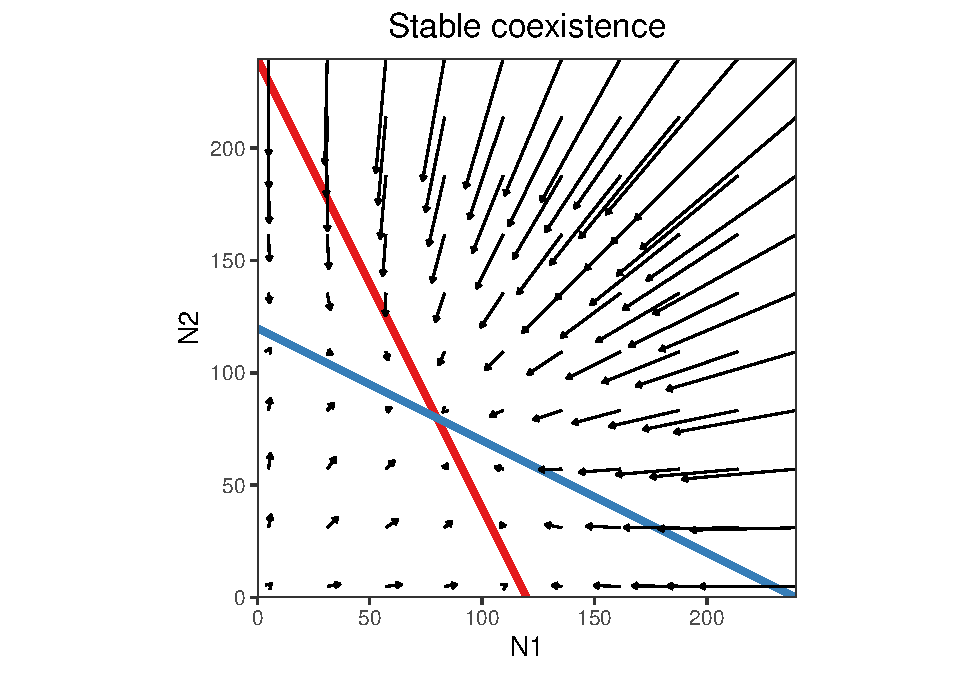
\includegraphics{bookdown-demo_files/figure-latex/unnamed-chunk-40-1.pdf}

\begin{Shaded}
\begin{Highlighting}[]
  \FunctionTok{phase\_plane}\NormalTok{(}\AttributeTok{r1 =} \FloatTok{1.2}\NormalTok{, }\AttributeTok{r2 =} \FloatTok{1.2}\NormalTok{, }
              \AttributeTok{a11 =} \DecValTok{1}\SpecialCharTok{/}\DecValTok{200}\NormalTok{, }\AttributeTok{a21 =} \DecValTok{1}\SpecialCharTok{/}\DecValTok{100}\NormalTok{, }\AttributeTok{a22 =} \DecValTok{1}\SpecialCharTok{/}\DecValTok{200}\NormalTok{, }\AttributeTok{a12 =} \DecValTok{1}\SpecialCharTok{/}\DecValTok{100}\NormalTok{, }
              \AttributeTok{t =} \FloatTok{0.2}\NormalTok{, }\AttributeTok{title =} \StringTok{"Unstable coexistence (saddle)"}\NormalTok{)}
\end{Highlighting}
\end{Shaded}

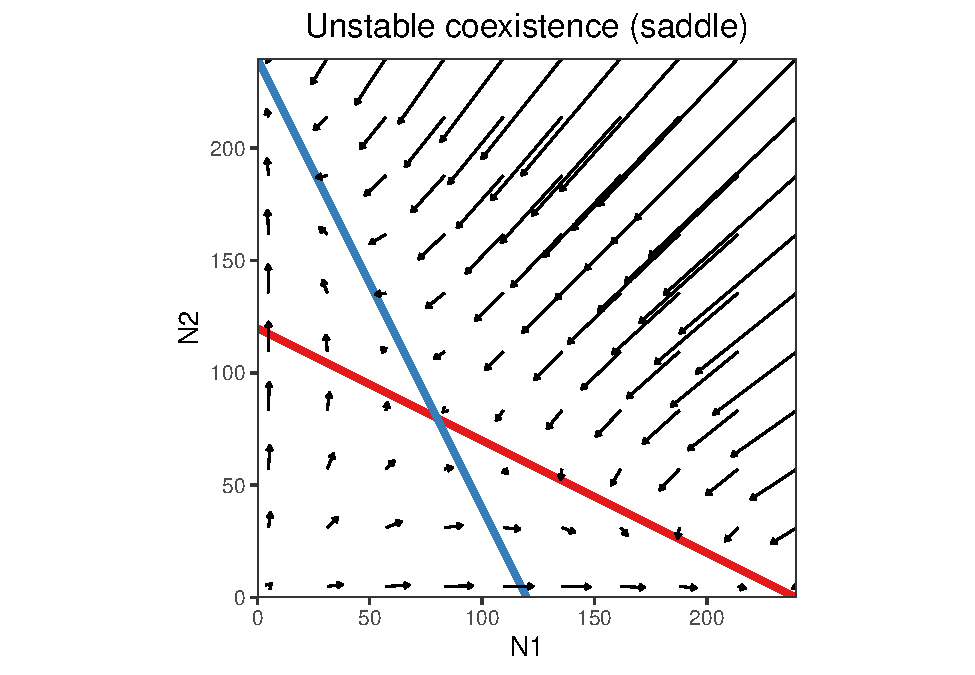
\includegraphics{bookdown-demo_files/figure-latex/unnamed-chunk-40-2.pdf}

\begin{Shaded}
\begin{Highlighting}[]
  \FunctionTok{phase\_plane}\NormalTok{(}\AttributeTok{r1 =} \FloatTok{1.2}\NormalTok{, }\AttributeTok{r2 =} \FloatTok{1.2}\NormalTok{, }
              \AttributeTok{a11 =} \DecValTok{1}\SpecialCharTok{/}\DecValTok{200}\NormalTok{, }\AttributeTok{a21 =} \DecValTok{1}\SpecialCharTok{/}\DecValTok{100}\NormalTok{, }\AttributeTok{a22 =} \DecValTok{1}\SpecialCharTok{/}\DecValTok{100}\NormalTok{, }\AttributeTok{a12 =} \DecValTok{1}\SpecialCharTok{/}\DecValTok{200}\NormalTok{, }
              \AttributeTok{t =} \FloatTok{0.2}\NormalTok{, }\AttributeTok{title =} \StringTok{"N1 wins"}\NormalTok{)}
\end{Highlighting}
\end{Shaded}

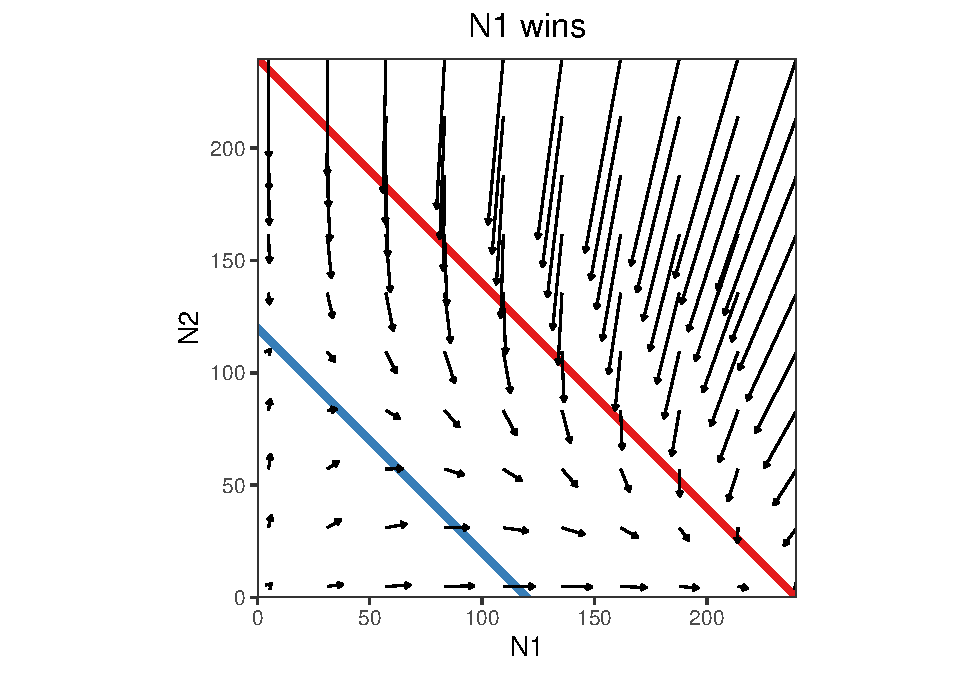
\includegraphics{bookdown-demo_files/figure-latex/unnamed-chunk-40-3.pdf}

\begin{Shaded}
\begin{Highlighting}[]
  \FunctionTok{phase\_plane}\NormalTok{(}\AttributeTok{r1 =} \FloatTok{1.2}\NormalTok{, }\AttributeTok{r2 =} \FloatTok{1.2}\NormalTok{, }
              \AttributeTok{a11 =} \DecValTok{1}\SpecialCharTok{/}\DecValTok{100}\NormalTok{, }\AttributeTok{a21 =} \DecValTok{1}\SpecialCharTok{/}\DecValTok{200}\NormalTok{, }\AttributeTok{a22 =} \DecValTok{1}\SpecialCharTok{/}\DecValTok{200}\NormalTok{, }\AttributeTok{a12 =} \DecValTok{1}\SpecialCharTok{/}\DecValTok{100}\NormalTok{, }
              \AttributeTok{t =} \FloatTok{0.2}\NormalTok{, }\AttributeTok{title =} \StringTok{"N2 wins"}\NormalTok{)}
\end{Highlighting}
\end{Shaded}

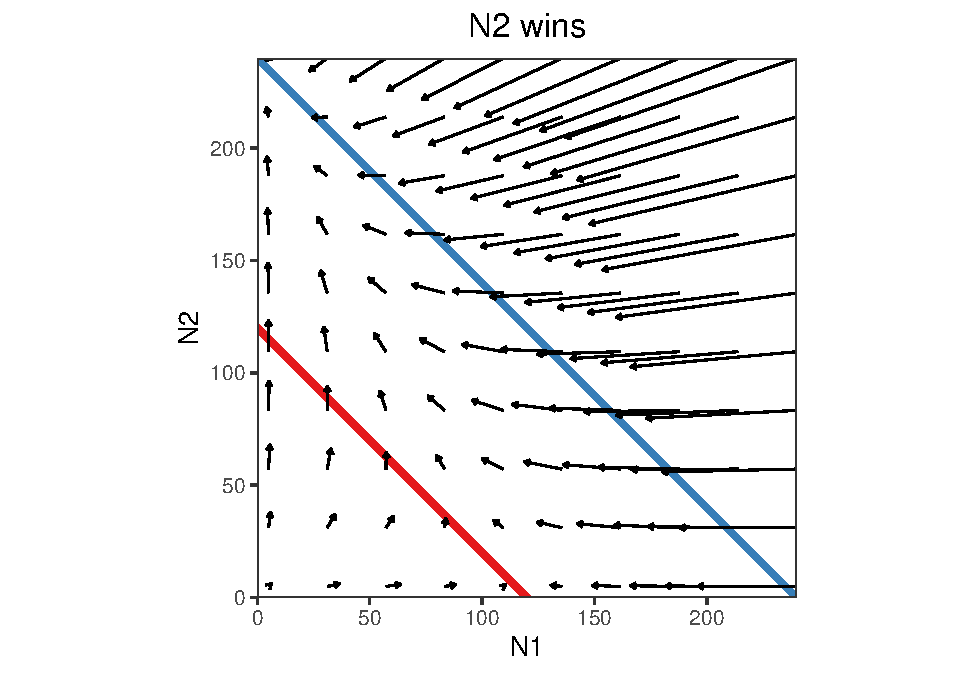
\includegraphics{bookdown-demo_files/figure-latex/unnamed-chunk-40-4.pdf}

  \bibliography{book.bib,packages.bib}

\end{document}
